% Stanford University PhD thesis style -- modifications to the report style
% This is unofficial so you should always double check against the
% Registrar's office rules
% See http://library.stanford.edu/research/bibliography-management/latex-and-bibtex
% 
% Example of use below
% See the suthesis-2e.sty file for documentation
%
\documentclass{report}

\usepackage[breakable]{tcolorbox}
\usepackage{parskip} % Stop auto-indenting (to mimic markdown behaviour)

\usepackage{iftex}
\ifPDFTeX
\usepackage[T1]{fontenc}
\usepackage{mathpazo}
\else
\usepackage{fontspec}
\fi

% Basic figure setup, for now with no caption control since it's done
% automatically by Pandoc (which extracts ![](path) syntax from Markdown).
\usepackage{graphicx}
% Maintain compatibility with old templates. Remove in nbconvert 6.0
\let\Oldincludegraphics\includegraphics
% Ensure that by default, figures have no caption (until we provide a
% proper Figure object with a Caption API and a way to capture that
% in the conversion process - todo).
\usepackage{caption}
\DeclareCaptionFormat{nocaption}{}
\captionsetup{format=nocaption,aboveskip=0pt,belowskip=0pt}

\usepackage[Export]{adjustbox} % Used to constrain images to a maximum size
\adjustboxset{max size={0.9\linewidth}{0.9\paperheight}}
\usepackage{float}
\floatplacement{figure}{H} % forces figures to be placed at the correct location
\usepackage{xcolor} % Allow colors to be defined
\usepackage{enumerate} % Needed for markdown enumerations to work
\usepackage{geometry} % Used to adjust the document margins
\usepackage{amsmath} % Equations
\usepackage{amssymb} % Equations
\usepackage{textcomp} % defines textquotesingle
% Hack from http://tex.stackexchange.com/a/47451/13684:
\AtBeginDocument{%
	\def\PYZsq{\textquotesingle}% Upright quotes in Pygmentized code
}
\usepackage{upquote} % Upright quotes for verbatim code
\usepackage{eurosym} % defines \euro
\usepackage[mathletters]{ucs} % Extended unicode (utf-8) support
\usepackage{fancyvrb} % verbatim replacement that allows latex
\usepackage{grffile} % extends the file name processing of package graphics 
% to support a larger range
\makeatletter % fix for grffile with XeLaTeX
\def\Gread@@xetex#1{%
	\IfFileExists{"\Gin@base".bb}%
	{\Gread@eps{\Gin@base.bb}}%
	{\Gread@@xetex@aux#1}%
}
\makeatother

% The hyperref package gives us a pdf with properly built
% internal navigation ('pdf bookmarks' for the table of contents,
% internal cross-reference links, web links for URLs, etc.)
\usepackage{hyperref}
% The default LaTeX title has an obnoxious amount of whitespace. By default,
% titling removes some of it. It also provides customization options.
\usepackage{titling}
\usepackage{longtable} % longtable support required by pandoc >1.10
\usepackage{booktabs}  % table support for pandoc > 1.12.2
\usepackage[inline]{enumitem} % IRkernel/repr support (it uses the enumerate* environment)
\usepackage[normalem]{ulem} % ulem is needed to support strikethroughs (\sout)
% normalem makes italics be italics, not underlines
\usepackage{mathrsfs}
\usepackage{outlines}

% The preceding line is only needed to identify funding in the first footnote. If that is unneeded, please comment it out.
\usepackage{cite}
\usepackage{amsmath,amssymb,amsfonts}
\usepackage{algorithmic}
\usepackage{graphicx}
\usepackage{amsmath}
\usepackage{nth}
\usepackage{todonotes}
\usepackage{url}
\usepackage{xcolor}
\usepackage{textcomp}
\usepackage{float}
\usepackage{subcaption}
\usepackage{cleveref}
\usepackage{listings}
%\usepackage[caption=false,font=footnotesize]{subfig}
%\usepackage[export]{adjustbox}

\newcommand*\rot{\rotatebox{90}}

\def\BibTeX{{\rm B\kern-.05em{\sc i\kern-.025em b}\kern-.08em
		T\kern-.1667em\lower.7ex\hbox{E}\kern-.125emX}}
	
\usepackage{suthesis-2e}
\dept{Computer Science}

\begin{document}
\title{Energy aware HPC}
\author{Vitor Ramos Gomes da Silva}
\principaladviser{Carlos Valderrama}
\coprincipaladviser{Pierre MANNEBACK}
\firstreader{Thierry DUTOIT}
\secondreader{Sidi MAHMOUDI}
\thirdreader{Samuel Xavier de Souza} %if needed
 
\beforepreface
\prefacesection{Preface}
Second Phd Committee
%\prefacesection{Acknowledgments}
%I would like to thank...
\afterpreface

\chapter{Introduction}
Energy consumption is a key to enable exascale High-performance Computing (HPC). Energy-optimized hardware and software combinations still could be inefficient if software operates poorly. 
Software operation relies on dynamic scaling of frequency and voltage (DVFS) as well as dynamic power management (DPM), but none have priority information on the application, which leads to inefficient software operation. This work proposes an analytical model that can be used to estimate energy-optimal software operation. 
This work proposes a new energy model that can be used as a basis to optimize DVFS and DPM, as well as to assess the contribution of parameters such as parallelism level and dynamic power to the energy consumption.
Since in HPC, applications can run on multiple cores and associated frequencies, both of which can be controlled for most systems, the novelty of the model includes such parameters as well as the workload, two application parameters and three system parameters.

\section{Motivation} \label{sec:motivation}
Data center energy efficiency has become of crucial importance in recent years due to its high economic, environmental, and performance impact. For example, the leading petaflop supercomputers consume a range of 1–18 MW of electrical power, with 1.5 MW on average, which can be easily translated into millions of dollars per year in electricity bills \cite{Group2012HandbookSahni}.
Data center energy consumption was estimated to be between 1.1\% and 1.5\% of worldwide electricity usage in 2010 \cite{Dayarathna2016DataSurvey,Corcoran2017EmergingICT}, generating as much pollution as a nation such as Argentina  \cite{Mathew2012Energy-awareNetworks}.
In some cases, the power costs exceed the cost of purchasing hardware~\cite{Rivoire2007ModelsOptimizations}.
Furthermore, the energy costs of powering a typical data center doubles every five years~\cite{Buyya2013Introduction}.
Therefore, with such a steep increase in power use, electricity bills have become a significant expense for today's data centers \cite{Poess2008EnergyCenters,Gao2013QualityCenters}. 
For these reasons, data center energy efficiency is now considered a primary concern for data center operators, often ahead of the traditional considerations of availability and security.

There are several approaches for green computing, from electrical materials to circuit design, systems integration, and software. These techniques may differ, but they share the same goal---to substantially reduce overall system energy consumption without a corresponding negative impact on delivered performance.
The processor and main memory are  the components that usually dominate power consumption, as shown in \cref{fig:powerbreakdown}.
The processor can consume as much as 50\% of the total energy~\cite{Fan2007PowerComputer, Barroso2007TheComputing, Malladi2012TowardsDRAM}. For that reason, modern processors incorporate several features for power management~\cite{Rotem2012Power-managementBridge, Brown2005ACPILinux, Hackenberg2015AnProcessor, Intel20200thLake}, such as dynamic power management (DPM) and dynamic voltage and frequency scaling (DVFS). 
DPM encompasses a set of techniques for obtaining energy-efficient computing by deactivating or reducing the system components' performance when they are idle or partially utilized~\mbox{\cite{Shuja2012Energy-efficientCenters, Benini2000AManagement}}.
DVFS allows the frequency and voltage to be adjusted in run-time depending on current needs.


\begin{figure}[H]
	\centering
	\captionsetup[subfigure]{justification=centering}
	
	\begin{subfigure}[b]{0.45\textwidth}
		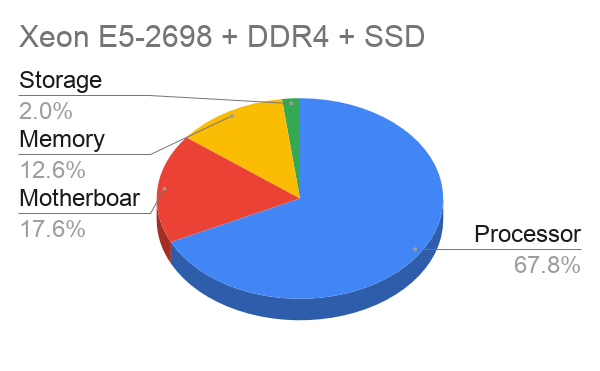
\includegraphics[width=\textwidth]{models/figures/power_breakdown/Xeon E5-2698 + DDR4 + SSD.png}
		\caption{}
		\label{fig:powerbreakdown_a}
	\end{subfigure}
	%
	\begin{subfigure}[b]{0.45\textwidth}
		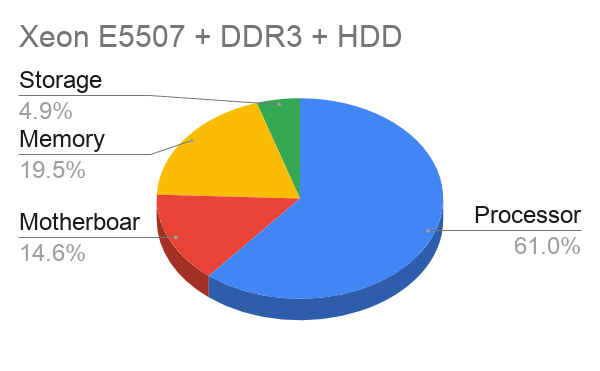
\includegraphics[width=\textwidth]{models/figures/power_breakdown/Xeon E5507 + DDR3 + HDD.png}
		\caption{}
		\label{fig:powerbreakdown_b}
	\end{subfigure}
	
	\hfill
	\caption{Power breakdown of a typical node of an HPC cluster at full use. The system used in this study (\textbf{a}) was built in 2016 and equipped with two Intel Xeon E5-2698, 128 GB of DDR4 memory and SSD as storage, while (\textbf{b}) the case study in \cite{Malladi2012TowardsDRAM} was built in 2012 and equipped with two Xeon E5507, 32GB of DDR3 memory and HDD as storage.}
	\label{fig:powerbreakdown}
\end{figure}

DVFS is motivated by the well-known fact that frequency and power have a near-cubic relationship \cite{Dayarathna2016DataSurvey, Group2012HandbookSahni}; this implies that running the CPU at a lower frequency causes a linear reduction in performance and a near-cubic reduction in power, which could lead to a near-square reduction in CPU energy.
Because of this, it is possible to achieve dramatic energy savings just with frequency control, depending on the system and its architecture.
Although very promising, the system software has yet to determine when and what voltage and frequency to use when running applications.
Otherwise, not only will performance deteriorate, but, in the worst case, energy consumption would also increase  \cite{Group2012HandbookSahni}.
Indeed, reducing the frequency results in a longer execution time, which increases the energy consumption of other system components, such as memory and disks.
There is also an overhead of time and energy associated with a voltage and frequency switch that needs to be considered.
Thus, finding the most appropriate voltage and frequency to use in all circumstances is not easy.
Therefore, since its introduction in 1994 \cite{Group2012HandbookSahni}, there has been a tremendous amount of research on DVFS algorithms.

The DPM technique can achieve substantial energy savings on systems where the static power is high, or the system remains inactive for a long time.
In that case, the problem is to determine when and which components to turn on/off.
With DPM, energy savings of 70\% have been reported~\cite{Shuja2012Energy-efficientCenters, Benini2000AManagement}. 

However, at the same time, while these power-saving techniques reduce system energy, they can compromise  performance leading  to a complex trade-off that needs to be carefully exploited to produce more energy-efficient algorithms.
Indeed, this study investigates whether the construction of an energy consumption model of an application can lead to significant energy savings.

We propose an analytical energy model for a given application in the function of the two control variables present in most HPC systems: CPU operating frequency and number of active cores. The model is composed of three application-dependent parameters and three parameters relating to the architecture of the system. The application parameters incorporate characteristics of the percentage of parallelism and the input size. The system architecture parameters include power-related and technology-dependent components, such as dynamic, static, and leakage power.

\section{Objectives}


\section{Contributions}

Although much work has been done on DVFS, the focus is still on the consumer electronics and laptop markets. 
For HPC, the notion of energy perception is relatively new~\cite{Feng2003MakingSupercomputing}. 
Moreover, the operational characteristics of non-HPC and HPC systems are significantly different. 
First, the workload on non-HPC systems is very interactive with the end-user, but the workload on the HPC platform is not.
Second, activities conducted on a non-HPC platform tend to share more machine resources.
In contrast, in HPC, each job often runs with dedicated resources. 
Third, an HPC system is usually much larger than a non-HPC system, making it more challenging to gather information, organize, and execute global decisions.
Therefore, it is worthwhile to investigate whether a DVFS scheduling algorithm, which works well for conventional computing, remains effective for HPC.

Our paper proposes a full-system energy model based on the CPU frequency and the number of cores. The model aims to understand and optimize the energy behavior of parallel applications in HPC systems according to application parameters, such as the degree of parallelism and CPU parameters related to dynamic and static power. The proposed model differs from existing ones, including the frequency and number of cores in the same equation for estimating the energy for a specific application in a given configuration. This model can serve as a base for considering DVFS and DPM optimization problems, including frequency and active cores. It can also be used to analyze the contribution of each parameter (ex: level of parallelism) to energy consumption. Furthermore, the number of cores is essential in HPC since applications are designed to run on multiple cores.

The proposed energy model is the product of an application-agnostic power model and an architecture-specific application performance model. The power model is based on the CMOS logic gates power draw as a function of the frequency~\cite{Sarwar1997CmosCalculation, Butzen2007LeakageGates} augmented to include the number of cores. The performance model is based on Amdahl's law \cite{Amdahl1967ValidityCapabilities, Eyerman2010ModelingDesign, Gustafson1988ReevaluatingLaw}, which can be used to estimate runtime in multi-core systems. In addition, this model has been extended to include execution frequency and input size, characterizing the application on the target architecture.


\cref{tab:related_work} summarizes the models comparing the system dependencies and the controllable variables.
\begin{table}[H]
	\footnotesize
	\caption{Related work summary.\label{tab1}}
	\setlength{\tabcolsep}{2.3mm}\begin{tabular}{cccc}
		\toprule
		%\begin{adjustwidth}{-\extralength}{0 cm}
		
		\textbf{Model}  & \textbf{System Dependency}       & \textbf{Variable}                     & \textbf{Controllable Variables}         \\ \midrule
		Merkel et al. \cite{Merkel2006BalancingSystems} & performance counters    & number of activities & - \\
		Roy et al. \cite{Roy2013AnAlgorithms}&performance counters &io operations, total time    & - \\
		Yakun et al. \cite{Shao2013EnergyProcessor}&number of instructions &frequency&frequency \\
		Lewis et al. \cite{Lewis2008Run-timeSystems}&energy of subcomponents&energy of subcomponents & - \\
		Mills et al. \cite{Mills2014EnergySystems}&power of subcomponents&total time, frequency & frequency \\ 
		Our model & - & frequency, cores, input size & frequency, cores, input size\\ \bottomrule
	\end{tabular}
	%\caption{Related work summary}
	\label{tab:related_work}
	%\bottomrule
\end{table}

The main contributions of the proposed model are:


% Contribuições por capitulo...
\begin{itemize}
	\item Simple model: faster to fit and compute, good for DVFS and DPM optimization.
	\item Parameters with logical meaning: helps to understand the contribution of each specific term.
	\item Analytical analysis: several analyses can be derived from the equation.
	\item Controllable variables: the equation is in the function of parameters that we can control directly.
\end{itemize}

\section{Organization}

%\chapter{Approch}
%
\section{Energy-Optimal Configurations for Single-Node HPC Applications\\
%{\footnotesize \textsuperscript{*}Note: Sub-titles are not captured in Xplore and should not be used}
%\thanks{Identify applicable funding agency here. If none, delete this.}
}

% Energy efficiency is a growing concern for modern computing, especially for High-Performance Computing (HPC) due to operational costs and the environmental impact. We propose a methodology to find the best energy-efficient configurations to run single-node applications in an HPC environment using an application-agnostic power model of the architecture and an architecture-aware performance model of the application. The operating frequency and number of active cores are the configuration parameters. This method differs from frequency scaling algorithms that do not have any previous information on the performance behavior of the application or the power consumption profile of the architecture. We characterize the application performance using Support Vector Regression. The power consumption is estimated by modeling the dynamic and static power consumed by CMOS transistors using a computation-intensive program to stress the architecture. The estimated energy-optimal configuration is computed by minimizing the product of the power model and the performance model's outcomes. The results obtained using four PARSEC applications with five different inputs show that the proposed approach was able to find configurations that used about 14$\times$ less energy when compared to the worst case of the default Linux governor for voltage and frequency scaling. When compared to the best case of this governor, the proposed approach saved up to 23\% on energy consumption, with an overall average of 6\% less energy.
% 150 words abstract
Energy efficiency is a growing concern for modern computing, especially for HPC due to operational costs and the environmental impact, considering that processors have an important role in this energy consumption. In this work, we propose a methodology to find energy-optimal frequency and number of active cores to run single-node HPC applications using an application-agnostic power model of the architecture and an architecture-aware performance model of the application. We characterize the application performance using machine learning, specifically the "Support Vector Regression" algorithm. Besides that, the power consumption is estimated by modeling CMOS dynamic and static power without knowledge of the application. So, The energy-optimal configuration is estimated by minimizing the product these two models outcomes, the power model and the performance model. Then, the final model can be used to find better frequency and number of cores to aim energy efficiency application execution. Results were obtained for four PARSEC applications and, with five different inputs shows that the proposed approach used substantially less energy when compared to the DVFS governor, in best cases and worst cases.


\section{Introduction} \label{sec:introduction}
Processors are the main contributor to the power consumption of High-Performance Computing (HPC) servers. They contribute between 20 and 40\% to the total server’s power draw~\cite{Fan2007}. Google's servers showed that during peak utilization processors consumed about 42\% of the overall server’s power consumption~\cite{Barroso2007}. Reducing processor power consumption is an effective approach to reduce the whole system's power consumption.  Therefore, modern processors incorporate several features for power management such as independent processing cores that can be disabled by the operating system~\cite{Rotem2012}, clock gating techniques for reducing the dynamic power dissipation of synchronous circuits~\cite{Srinivasan2015} and Dynamic Voltage and Frequency Scaling (DVFS)~\cite{Mittal2014}.

DVFS has been demonstrated to be a very effective technique for reducing the power consumption of processors \cite{Hackenberg2015, Dzhagaryan2014, Hahnel2012, Basmadjian2012, Travers2015, Miyoshi2002, Anghel2011, Pietri2014}. The technique tries to optimize power consumption by adjusting the frequency according to the current load of the processor. Generally, the frequency scales with the intensity of the load and the voltage scales to the minimum value that enables the selected frequency. Among other aspects, DVFS helps in reducing energy consumption because it allows memory-bounded programs to be executed more efficiently \cite{Spiga2006}. Nonetheless, aspects such as load variability may compromise the effectiveness of DVFS. Another important aspect that is typically not taken into account is the number of processing cores to be used by a parallel program. This choice is left to the user, which often is not trivial as shown in this paper.% the power consumption but increasing the execution time. This way is not guaranteed that the energy consumption will be the lower since energy depends on the power and time, there might be a configuration with higher power consumption that can lead to less energy consumed because of the execution time is lower.

We propose a methodology to find the operating frequency and number of active cores that minimize the total energy used to execute an HPC application on a single shared-memory HPC node.

The methodology uses an application-agnostic power model and an architecture-specific application characterization to model performance. The power model is based on the modeling of Complementary Metal-Oxide-Semiconductor (CMOS) logic in the function of the operating frequency \cite{Sarwar1997}. It models both dynamic and static power. Besides operating frequency, the power model is also parametric to the number of active sockets and the number of active cores per socket. 

Performance is modeled by characterizing the application on the target architecture. The idea is to predict the performance of the application at any given configuration. The model takes as inputs the operating frequency, the number of active cores and the input size. The modeling is done using a supervised learning method for regression called Support Vector Regression (SVR)~\cite{Smola2004}.

To find the optimal-energy configurations, the algorithm minimizes the product of outcomes of the power and performance models. This approach was validated on four PARSEC applications~\cite{Bienia2008} and compared to the \emph{Ondemand} governor, which is the default DVFS scheme for the Linux operating system. The results show that the proposed approach was able to find configurations that used about 14$\times$ less energy when compared to the worst case of the Ondemand governor. When compared to the best case of this DVFS scheme, i.e. when the user guesses the optimal number of cores to be used, the proposed approach was able to find configurations that used as much as 18.7\% less energy to execute the target application. The overall average energy saving reached 5.7\% for the proposed approach when compared to the best case and 88.8\% when compared to the worst case.

% TODO: Terminar de detalhar quando fechar a versão final das seções

The rest of this paper is organized as follows. Section~\ref{sec:models} presents the proposed models for power, performance, and energy. The experimental setup and the fitting of the models are described in Section~\ref{sec:experimentalsetup}. In Section~\ref{sec:experimentsresults}, the results of applying the proposed approach to four PARSEC applications are presented. Related works are presented in Section~\ref{sec:relatedwork}. Finally, conclusions are drawn and future work is proposed in Section\ref{sec:conclusion}.

% \section{Theoretical background} \label{Theoretical_background}
% %In the following subsections we present a background on how the DVFS control works and describe how to monitor of power information in real time.

% \subsection{DVFS} \label{DVFS}
% The DVFS implementation complies with the Advanced Configuration and Power Interface (ACPI) \cite{Wikipedia2010} standard which is adopted by operating systems to configure hardware components related to power management. In this standard two states are defined, the C and P states, which are important to the processor frequency and voltage control.

% The C state optimizes the power consumption when the processor is not executing any instructions. This state has several levels. The processor initially starts at C0 level, where the Central Processing Unit (CPU) is fully activated. If the CPU is idle for a specified time, then it moves to the next level, C1, where some CPU functionalities are disabled. After spending some time on the C1 level, the processor passes to the next level where more functionalities are disabled, and so on. ACPI defines four levels, but, manufacturers can define additional ones.

% The P state optimizes the voltage and the frequency during the active execution. It starts at the P0 level, with the highest frequency and voltage possible.  At the P1 level, both the frequency and voltage are decreased, and this goes on until the last level is reached with the lowest possible values. The ACPI standard does not specify the number of the P levels, so this is a manufacturers' choice.

% The P and C states can be controlled by interfaces mediated by drivers available on the operating system. The Linux kernel has many drivers available developed by the CPU manufacturers and the community \cite{Brown2005}. The default driver is the "acpi-cpufreq'' that uses policies implemented by so-called governors that dynamically decide the frequency values. Some of the governors available are Performance, Powersave, Ondemand, Conservative and Userspace. Performance and Powersave are static, and they set the frequency to the maximum and minimum allowed values, respectively. Ondemand and Conservative implementing algorithms to estimate the CPU required capacity and adjust the processor frequency accordingly. Finally, Userspace allows the user to specify the frequency.

% \subsection{IPMI} \label{IPMI}

% The Intelligent Platform Management Interface(IPMI) is a set of interfaces used by HPC system administrators. These allow for out-of-band management of computer systems and platform-status monitoring through local network \cite{November2013}. It can monitor variables and resources such as the system's temperature, voltage, fans and power supplies, with independent sensors attach to the hardware.

% The system consists of the main controller, called the baseboard management controller (BMC), and other management controllers distributed among different system modules, as shown in figure \ref{fig:ipmi_diagram}.

% \begin{figure}[H]
% \centerline{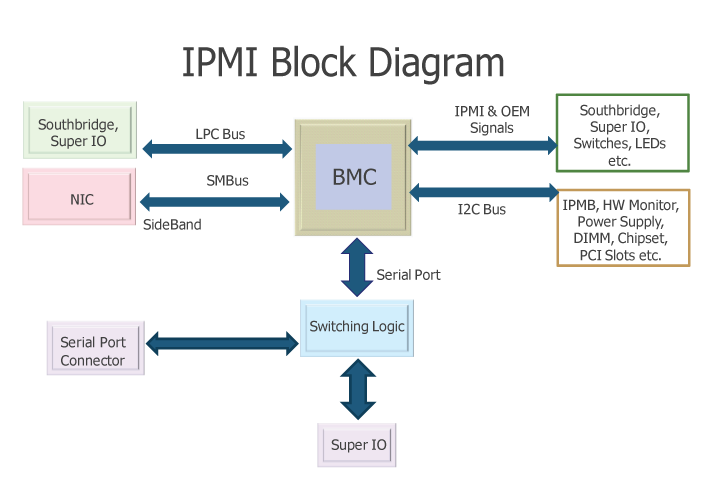
\includegraphics[width=\columnwidth]{figures/IPMI-Block-Diagram.png}}
% \caption{IPMI block diagram, this image was taken from http://pt.wikipedia.org }
% \label{fig:ipmi_diagram}
% \end{figure}

% %The BMC operate independent of the operating system and his access can be through HTTP protocol or using a tool provided by the manufacturer.

\section{Models} \label{sec:models}
In this Section, we present the proposed power and performance models that are used to estimate the minimum-energy consumption configuration.

\subsection{Power Model} \label{sec:powermodel}
Some of the main factors that contribute to the CPU power consumption are the dynamic power consumption, the short-circuit power consumption, and the power loss due to the current leakage of transistors, \cite{Rauber2014, Goel2016, Du2017, Gonzalez1997}. The complexity of the circuits of modern processors makes it very difficult to model their power consumption accurately. A viable approach for modeling the CPU's power draw is to model their building components, which are mainly made out of CMOS logic gates. Thus, modeling the power consumption for one logic gate and multiplying this by the total number of gates reduces the complexity of modeling the internal circuits but still provides the sufficient accuracy needed for making optimization decisions.

%The modern technology to construct logic gates is the CMOS, and t
There are three main components of power dissipation in digital CMOS circuits,
\begin{equation}
P_{total}=P_{static}+P_{leak}+P_{dynamic} \label{eq_totalPower},
\end{equation}
namely, static power $P_{static}$, dynamic power $P_{dynamic}$, and leakage power $P_{leak}$.
According to~\cite{Sarwar1997, Butzen2007}, the dynamic power, and leakage power behavior can be approximated by:
\begin{equation}
P_{dynamic}=CV^2f \quad \text{and} \quad P_{leak} \propto V
\label{eq_draws}
\end{equation}
% and
% \begin{equation}
% \end{equation}
where $C$ is the CMOS capacitance, $V$ the voltage applied to the circuit and $f$ the switching frequency.

Another common approximation is to expect a linear relationship between the voltage and the applied frequency~\cite{Usman2013} $ f \propto V \label{eq_fapoxV} $. The static power in our model represents the energy consumed by other components of the CPU. Thus, the proposed model for one processing core of a multi-core processor is derived by using (\ref{eq_draws}) and (\ref{eq_fapoxV}) to rewrite (\ref{eq_totalPower}) as follows:

\begin{equation}
P_{total}(f)= c_1f^3+c_2f+c_3 \label{eq_fitting},
\end{equation}
where $c_1$, $c_2$, and $c_3$ are the model's parameters. When we include the number of active cores $p$, the estimation of the power consumption of the whole processor becomes:

%done \todo[inline]{You do not say what p is. I guess is processors or active cores?}

\begin{equation}
P_{total}(f,p)= p(c_1f^3+c_2f)+c_3 \label{eq_power_core},
\end{equation}
where the dynamic and leakage power parts are multiplied by the number of cores and the static power that is the consumption of other parts of the CPU remains the same. For systems that have more than one processor sockets, the power cost of enabling each socket can be considered. Adding the number of sockets $s$ to the equation gives the final version of the power model used in this work:
% done \todo[inline]{Is s the number of sockets rather than the power cost??}
\begin{equation}
P_{total}(f,p,s)= p(c_1f^3+c_2f)+c_3+c_4s \label{eq_power_final},
\end{equation}
with $c_4$ being the model parameter for the number of sockets.

\subsection{Performance Model} \label{sec:performancemodel}
The performance model aims to estimate the application's execution time for a given target architecture based on a given operating frequency, number of active cores and input size. 

The performance was modeled by sampling the execution time of the application for several combinations of discrete values of frequency, number of active cores and input size. The samples were used as a training set for a Support Vector Regression (SVR); a version of the Support Vector Machine (SVM) algorithm for regression proposed in~\cite{Drucker1997}. Training the SVR means minimize the weights $w$ subject to $|y_i-\langle w,x_i\rangle-b| \leq \varepsilon$.

% \[ \begin{cases} 
%       y_i-\langle w,x_i\rangle-b \leq \varepsilon \\
%       \langle w,x_i\rangle+b-y_i \leq \varepsilon \\
%   \end{cases}
% \]

In our model $x_i$ is a vector with the frequency, the number of active cores and input size, $y_i$ is the execution time measured. $\langle w,x_i\rangle+b-y_i$ is the predicted output time and $\varepsilon$ is a free parameter that serves as a threshold.

\subsection{Energy Model} \label{sec:energymodel}
By combining outcome of the power model described in~\cref{sec:powermodel} and the SVR characterization of the application performance described in \cref{sec:performancemodel}, we can estimate the total energy used by the application as follows:
\begin{equation}
E(f,p,s,N)=P(f,p,s)\times{\rm SVR}(f,p,N) \label{eq_energy},
\end{equation}
where $P(f,p,s)$ is the total power modeled by~(\cref{eq_totalPower}), ${\rm SVM}(f,p,N)$ is the execution time estimated by the SVR characterization of the application, $f$ is the frequency, $p$ is the number of active cores, $s$ is the number of sockets, and $N$ is the input size. 

%\todo[inline]{it is not obvious why you can estimate energy consumption rapidly}
With (\ref{eq_energy}), it is possible to calculate energy consumption estimations for every possible configuration. Then, the configuration that minimizes energy consumption for a given input can be selected. It is also possible to apply constraints on the execution time, frequency, and the number of active cores although this is not considered in this work.

%To calculate the minimum of this function any numeric minimization method can be used and the domain to search is well defined by the limitations of the system frequency, number of cores and sockets

\section{Experimental Setup} \label{sec:experimentalsetup}
%As discussed in the previous section, prior calculate the minimal energy, its necessary find the following models: Power model and Performance Model. Therefore, the experiments start obtaining these models of applications on platform chosen.   
In the following subsections we present the software and hardware experimental setup used to validate the proposed approach.

\subsection{Case-Study Applications} \label{sec:casestudyapplication}
% Ok \todo[inline]{no need to list all the areas PARSEC is covering as you only cope with 4 case studies I believe}
Four applications from the PARSEC parallel benchmark suite, version 3.0~\cite{Bienia2008}, were used as case studies. 
%These, cover an ample range of areas such as financial analysis, computer vision, engineering, enterprise storage, animation, similarity search, data mining, machine learning, and media processing, 
This suite focuses on emerging workloads and was designed to be representative of the next generation shared-memory programs for chip-multiprocessors. The four applications used in this work were chosen for being relatively straightforward to devise smaller input sizes from the standard native inputs. 
% , although the benchmark already provides different inputs they division doesn't scale in an exact proportional rate and some of them were too small for our experiments. 
These are Fuidanimate, Raytrace, Swaptions, and Blackscholes.
Since the other provided inputs were meant to evaluate simulated architectures, they are too small for measuring execution time in real machines.
% A short description of each one follows.

% \subsubsection{Blackscholes} calculates the prices for a portfolio of European options analytically using the Black-Scholes partial differential equation. There is no closed-form expression for the Black-Scholes equation and as such it must be computed numerically. The program's inputs are the number of threads, the input file containing the options data, and the output file name. %\todo{what do the input and output file contain?}

% \subsubsection{Fuidanimate} uses an extension of the Smoothed Particle Hydrodynamics (SPH) method to simulate an incompressible fluid for interactive animation purposes. The inputs are the number of threads, the number of frames, and an input file with information of all fluid particles and his proprieties.%\todo{again what does the input file has?}.

% \subsubsection{Raytrace} is a version of the raytracing method that is typically employed by real-time animations such as the ones used in computer games. It is optimized for speed rather than realism. The computational complexity of the algorithm depends on the resolution of the output image and the scene. The inputs used on this applications was the number of threads, the number of frames, a 3D object and the display resolution.

% \subsubsection{Swaptions} Uses the Heath-Jarrow-Morton (HJM) framework to price a portfolio of swaptions. Swaptions employs Monte Carlo (MC) simulation to compute the prices. The input to this program are the number of threads, number of swaptions and the number of trials.

\subsection{Case-Study Architecture} \label{sec:casestudyarchitecture}
% \todo[inline]{is the first sentence really necessary? if yes, NPAD and UFRN needs definition}
%In the experiments performed in this work, we used the compute nodes of the High-Performance Computing Center (NPAD/UFRN)\footnote{NPAD is the name of the High Performance Computing Center (from Portuguese: Núcleo de Processamento de Alto Desempenho) of the Universidade Federal do Rio Grande do Norte (UFRN).}. This HPC nodes consist 
In the experiments performed in this work, we used compute nodes that consists of two Intel Xeon E5-2698 v3 processors with sixteen cores each and two hardware threads for each core. The maximum non-turbo frequency is 2.3GHz, and the total physical memory of the node is 128GB (8$\times$16GB). Turbo frequency and hardware multi-threading were disabled during all experiments. The operating system used is Linux CentOS 6.5, kernel 2.6.32.

The Linux kernel has many drivers available developed by the CPU manufacturers and the community \cite{Brown2005}. The default driver is the "acpi-cpufreq'' that uses policies implemented by so-called governors that dynamically decide the frequency values. Some of the governors available are Performance, Powersave, Ondemand, Conservative and Userspace. Performance and Powersave are static, and they set the frequency to the maximum and minimum allowed values, respectively. Ondemand and Conservative implement algorithms to estimate the CPU required capacity and adjust the processor frequency accordingly. Finally, Userspace allows the user to specify the frequency.

In this work, changing the frequency of the cores was done using the Linux "acpi-cpufreq'' driver. The number of active cores was changed by modifying the appropriate Linux virtual files. Both changes require root privileges. In practice, this approach can be brought into production by allowing the resource manager to perform these changes for the user using pre- and post-scripts for job submissions with energy consumption requirements. We also assume that all processors run at the same frequency.

%To execute the experiments was necessary to change the frequency of cores and, also, turn off the cores not used on each step of execution. This was done by Operating System drivers, as acpi-cpufreq, and the Linux virtual files. On systems where not is possible change the frequency by Operating System, it is necessary to enable the frequency scaling by software on the BIOS.

\subsection{Fitting the Power Model} \label{sec:powerfitting}
To fit the power-model equation, the CPU was stressed up to 100\% with a special benchmark made for this purpose similar to the Linux tool stress. Power information was acquired from the Intelligent Platform Management Interface (IPMI) sensors which measures the energy consumption of the entire system at about one sample per second. IPMI provides information about variables and resources such as the system's temperature, voltage, fans, and power supplies; using independent sensors attach to the hardware.

% The system consists of the main controller, called the baseboard management controller (BMC), and other management controllers distributed among different system modules, as shown in figure \ref{fig:ipmi_diagram}.

% \begin{figure}[H]
% \centerline{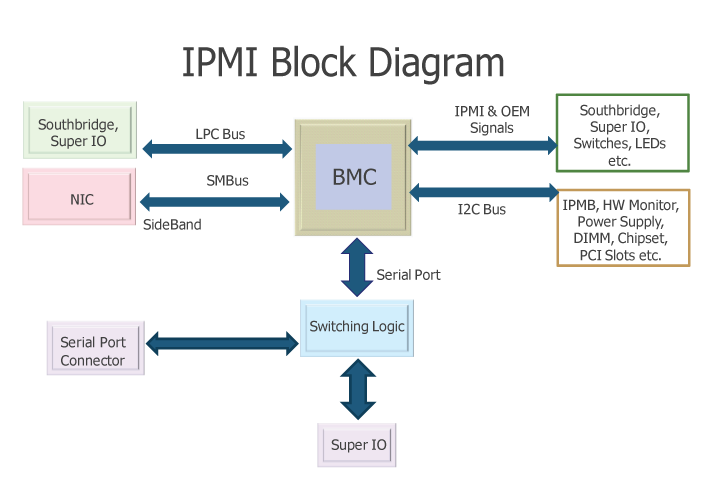
\includegraphics[width=\columnwidth]{figures/IPMI-Block-Diagram.png}}
% \caption{IPMI block diagram, this image was taken from http://pt.wikipedia.org }
% \label{fig:ipmi_diagram}
% \end{figure}

% %The BMC operate independent of the operating system and his access can be through HTTP protocol or using a tool provided by the manufacturer.

The power was collected for all combinations of frequency --- starting from 1.2~GHz and increasing by 100 MHz each time until 2.2~GHz is reached, and possible numbers of active cores --- from 1 to 32. Between each test, the CPU was left idle until it cooled down to avoid interference on the next test.

The coefficients of (\ref{eq_power_final}), $c_1$, $c_2$, $c_3$ and $c_4$, were found by performing multi-linear regression on the data collected. The retrieved fitting can be seen on Fig.~\ref{fig:fitting}.

\begin{figure}[H]
\centerline{\includegraphics[width=\columnwidth]{ch1/figures/power.png}}
\caption{Power model fitting. The dots represent real power measurements and the solid lines represents the modeled power.}
\label{fig:fitting}
\end{figure}

The fitted equation for estimating the power in the target architecture was:
\begin{equation} 
P_{total}(f,p,s)=p(0.29f^3+0.97f)+198.59+9.18s, \label{eq:fittedpower}
\end{equation}
where the unit for frequency is GHz.

To validate this model was calculated the absolute percentage error, i.e. the mean of the perceptual error on each point. This metric was chosen because of the significant difference between the smallest and the biggest values and it is calculated as follows:

\begin{equation}
\sum_{i}^{\rm \# samples}{\frac{|y_i-y_{\rm model}|}{y_i}}.
\label{mpe}
\end{equation}

The resulting minimum, mean, and maximum absolute percentage errors were 0.007\%, 0.75\%, and 2.6\% respectively. While the root mean squared error was 2.38 W.

\subsection{Performance Characterization} \label{sec:performancecharacterization}

To characterize an application, we ran it for all different numbers of active cores in the range of $1<=p<=32$, for all the frequencies in the range of $1.2<=f<=2.2$ using 100MHz steps, and for 5 different input sizes.

%depending on the application, the number of cores was different because some applications can only run with the power of 2 and others can only run with an even number of threads. 
% done, please check \todo[inline]{is this empirically chosen then? What is the reasoning of making such choices?not clear why this selection is useful}
The input sizes were chosen in such a way that the average execution time was in the order of minutes. The sampled power information, on every second, was used to calculate the real energy usage. The total time to complete the characterization varied between one and two days, depending on the application.

The SVR model was built using the collected data. A grid search was used to tune the model parameters. In this case, a Radial Base Function (RBF) kernel and the penalty for the wrong term of $10\times10^3$ and gamma 0.5 \cite{scikit-learn}. To train the SVR, the data collected was divided into two parts, 90\% for training and 10\% to test the accuracy.

The model was validated also using cross-validation $k$-fold with $k$ equal to 10, using the Mean Absolute Error (MAE) and Percentage Absolute Error (PAE) as metrics. The average results of the cross-validation can be seen in Table~\ref{tab:svr_evaluation}.

\begin{table}[H]
\centering
\caption{Performance-Model's Cross validation Errors}
\label{tab:svr_evaluation}
\begin{tabular}{|l|l|l|l|l|}
\hline
Application  & MAE & PAE \\ \hline
\hline
Blackscholes & 2.01  & 4.6\% \\ \hline
Fluidanimate & 6.65  & 1.89\% \\ \hline
Raytrace  & 3.77  & 0.87\% \\ \hline
Swaptions & 2.29  & 2.56\% \\ \hline
\end{tabular}
\end{table}

One of the results of the characterization can be seen in Figs.~\ref{fig:svr_time2}.
% ,~\ref{fig:svr_time3},~\ref{fig:svr_time4}, and ~\ref{fig:svr_time1}.

\begin{figure}[H]
	\centerline{\includegraphics[width=\columnwidth]{ch1/figures/time_fluid_4.png}}
    \caption{Fluidanimate's performance model. The dots represent real performance measurements and the solid lines represent the modeled performance for various numbers of active cores and frequencies when running for input size 3.}
	\label{fig:svr_time2}
\end{figure}

%\begin{figure}[H]
%\subfigure[Fluidanimate's performance model. The dots represent real performance measurements and the solid lines represent the modeled performance.]{%
%	\label{fig:svr_time2}
%	\centerline{\includegraphics[width=\columnwidth]{ch1/figures/time_fluid_4.png}}
%}%
%\end{figure}

% \begin{figure}[H]
% 	\centerline{\includegraphics[width=\columnwidth]{ch1/figures/time_rtview_3.png}}
% 	\caption{Raytrace's performance model. The dots represent real performance measurements and the solid lines represent the modeled performance for various numbers of active cores and frequencies when running for input size 3.}
% 	\label{fig:svr_time3}
% \end{figure}


%\begin{figure}[H]
%\subfigure[Raytrace's performance model. The dots represent real performance measurements and the solid lines represent the modeled performance.]{%
%	\label{fig:svr_time3}
%	\centerline{\includegraphics[width=\columnwidth]{ch1/figures/time_rtview_3.png}}
%}%
%\end{figure}

% \begin{figure}[H]
% 	\centerline{\includegraphics[width=\columnwidth]{ch1/figures/time_swap_3.png}}
% 	\caption{Swaptions's performance model. The dots represent real performance measurements and the solid lines represent the modeled performance for various numbers of active cores and frequencies when running for input size 3.}
% 	\label{fig:svr_time4}
% \end{figure}

%\begin{figure}[H]
%\subfigure[Swaptions performance model. The dots represent real performance measurements and the solid lines represent the modeled performance.]{%
%	\label{fig:svr_time4}
%	\centerline{\includegraphics[width=\columnwidth]{ch1/figures/time_swap_3.png}}
%}%
%\end{figure}

% \begin{figure}[H]
% 	\centerline{\includegraphics[width=\columnwidth]{ch1/figures/time_black_4.png}}
%     \caption{Blackscholes's performance model. The dots represent real performance measurements and the solid lines represent the modeled performance for various numbers of active cores and frequencies when running for input size 3.}
% 	\label{fig:svr_time1}
% \end{figure}

%\begin{figure}[H]
%\subfigure[Blackscholes performance model. The dots represent real performance measurements and the solid lines represent the modeled performance.]{%
%	\label{fig:svr_time1}
%	\centerline{\includegraphics[width=\columnwidth]{ch1/figures/time_black_4.png}}
%}%
%\caption{SVR performance modeling plots for four PARSEC applications. The plots present the modeled and the measured performances for various numbers of active cores and frequencies when running for the mid-size input.}
%\end{figure}
%\todo{mid-size input?}

\section{Experimental Results} \label{sec:experimentsresults}
%As mentioned previously, the aim of this work is to obtain the optimal energy configuration on a parallel application running on a homogeneous platform. In general, the actual solutions are using the DVFS techniques to minimize energy consumption. The following shows the results obtained with the proposed approach.
In this Section, we present results for the energy model that we introduced in Section~\ref{sec:models} based on the parameter fitting described in Sections~\ref{sec:powerfitting} and~\ref{sec:performancecharacterization}. First, we compare and comment on the model in contrast with the actual energy measurements. Finally, we evaluate the effectiveness of the proposed approach by comparing it to the Linux default Ondemand DVFS governor.

\subsection{Measured versus Modeled Energy} \label{sec:measuredversusmodeledenergy}
The energy measurements were obtained by integrating the power measurements over the total execution time of the application.
The power measurements were made using the IPMI sensors with a sampling rate of about one sample per second.
% \todo[inline]{move mode details about IPMI here}

%From energy equation (\ref{eq_energy}), running the parsec applications and using the proposed model, it can be observed a compensation of energy consumption, depending on how application scales, between the growth of the number of cores and the associated decrease on execution time due to the parallelization. So, the results shows that the power consumption does not vary very much, as can see on figures 
Figs. \ref{fig:rt_s3}, and~\ref{fig:swap_s3}
%\ref{fig:fluid_s3}, \ref{fig:black_s3}
plot the measured and modeled energy consumption for Raytrace and Swaptions, respectfully, for varying the number of active cores and operating frequency, running with the mid-size input.

% \begin{figure}[H]
% 	\centerline{\includegraphics[width=\columnwidth]{ch1/figures/fluid_4.png}}
%     \caption{Fluidanimate's energy measurements versus modeled energy consumption  varying the number of active cores and operating frequency, running with the input size 3.}
% 	\label{fig:fluid_s3}
% \end{figure}

%\begin{figure}[H]
%\subfigure[Fluidanimate's energy measurements versus modeled energy consumption]{%
%	\label{fig:fluid_s3}
%	\centerline{\includegraphics[width=\columnwidth]{ch1/figures/fluid_4.png}}
%}%
%\end{figure}


\begin{figure}[h]
	\centerline{\includegraphics[width=\columnwidth]{ch1/figures/rtview_3.png}}
    \caption{Raytrace's energy measurements versus modeled energy consumption  varying the number of active cores and operating frequency, running with the input size 3.}
	\label{fig:rt_s3}
\end{figure}

%\begin{figure}[H]
%\subfigure[Raytrace's energy measurements versus modeled energy consumption]{%
%	\label{fig:rt_s3}
%	\centerline{\includegraphics[width=\columnwidth]{ch1/figures/rtview_3.png}}
%}%
%\end{figure}

\begin{figure}[h]
	\centerline{\includegraphics[width=\columnwidth]{ch1/figures/swap_3.png}}
    \caption{Swaptions's energy measurements versus modeled energy consumption  varying the number of active cores and operating frequency, running with the input size 3.}
	\label{fig:swap_s3}
\end{figure}

%\begin{figure}[H]
%\subfigure[Swaptions' energy measurements versus modeled energy consumption]{%
%	\label{fig:swap_s3}
%	\centerline{\includegraphics[width=\columnwidth]{ch1/figures/swap_3.png}}
%}%
%\end{figure}


% \begin{figure}[H]
% 	\centerline{\includegraphics[width=\columnwidth]{ch1/figures/black_4.png}}
%     \caption{Blackscholes's energy measurements versus modeled energy consumption varying the number of active cores and operating frequency, running with the input size 3.}
% 	\label{fig:black_s3}
% \end{figure}

%\begin{figure}[H]
%\subfigure[Blackscholes' energy measurements versus modeled energy consumption]{%
%	\label{fig:black_s3}
%	\centerline{\includegraphics[width=\columnwidth]{ch1/figures/black_4.png}}
%}%
%\caption{Measured and modeled energy consumption for four PARSEC applications for varying the number of active cores and operating frequency, running with the mid-size input.}
%\end{figure}

%Looking at the same frequency, the energy consumption has greater significance when the program runs with less active cores, but, even the difference being not very significant, the total energy of the best configuration always tend to happen on higher frequency because execution time decreases faster than power increases when raising the frequency. This relation can change depending on the power consumption of the system.
In general, for the case-study applications and case-study architecture, the optimal-energy configurations tend to be the ones using the highest frequency, which characterizes a race-to-idle rather than a pace-to-idle optimal behavior~\cite{kim2015racing}. This can be explained by the large static power observed in the considered architecture, evidenced by the large $c_3$ parameter in (\ref{eq_power_final}) that was fitted in (\ref{eq:fittedpower}). With a large static power, using a pace-to-idle strategy, i.e. the use of frequencies lower than the maximum, is expected to be effective only if the sum of the leakage and the dynamic power parcels is larger than the static power parcel. 
Based on the fitted power model, this would never happen, i.e. the sum of leakage and dynamic power is always less than the static power,
\begin{equation*}
p(0.29f^3+0.97f)+9.18s < 198.59,
\label{ineq:race_to_idle}
\end{equation*}
even if we use the maximum number of cores, $p=32$ and $s=2$, and the maximum frequency, $f=2.2$.

Nevertheless, race-to-idle is not always the best strategy for all systems because energy scales with the execution time, which in turn scales inversely with the number of active cores and the operating frequency, and because power scales linearly with the number of cores, but cubic with the frequency. For this reason, our proposal found optimal strategy for Raytrace and Blackscholes that are not the race-to-idle configuration, as we present in the next Subsection. 

The optimal number of active cores also depends on the parallel scalability of the application. The more scalable the application, the more cores it requires to minimize energy. A scalable application can increasingly exchange the speedup of more cores with lower frequencies in order to spend less energy. This is because of the linear relationship between power and number of cores and the exponential relationship between power and frequency.  

\subsection{Proposed Approach versus Ondemand Linux Governor}
\label{sec:proposedapproach}
We have compared the energy consumption of the four case-study applications using the energy-optimal configurations provided by the proposed approach to the energy consumption resulted by use of the Linux default DVFS governor, Ondemand. Since the governor does not choose the number of active cores, we executed each application using 1, 2, 4, 6, 8, $\cdots$, 28, 30, and 32 cores, accounting for the best and the worst cases of energy consumption. Tables \ref{tab:fluidfreq}, \ref{tab:raytracefreq}, \ref{tab:swapfreq} and \ref{tab:blackfreq} present these results for Fuidanimate, Raytrace, Swaptions, and Blackscholes, respectively. the maximum and minimum savings of the proposed approach in comparison with the Ondemand governor. The savings are calculated as follows: 
\begin{equation}
    \frac{100*({\rm Proposed}-{\rm Ondemand})}{\rm Ondemand}.
\end{equation}

\begin{table}[H]
\caption{Fluidanimate Minimal energy}
\label{tab:fluidfreq}
\resizebox{\columnwidth}{!}{%
\begin{tabular}{l|l|l|l|l|l|l|ll}
Input & \rot{\begin{tabular}[c]{@{}l@{}}Mean Freq. \\ in GHz \\ (\#Cores) \end{tabular}} & \rot{Energy in KJ} & \rot{\begin{tabular}[c]{@{}l@{}}Mean Freq. \\ in GHz \\ (\#Cores) \end{tabular}} & \rot{Energy in KJ} & \rot{\begin{tabular}[c]{@{}l@{}} Freq. \\ in GHz \\ (\#Cores) \end{tabular}} & \rot{Energy in KJ} & \multicolumn{1}{l|}{\rot{Min. Save(\%)}} & \rot{Max. Save(\%)} \\ \hline
1     & 1.85 (32)                                                                        & 4.85               & 2.29 (1)                                                                         & 32.38              & 2.0 (32)                                                                     & 4.15               & \multicolumn{1}{l|}{14.5}                & 87.2                \\ \hline
2     & 1.88  (32)                                                                       & 9.35               & 2.29 (1)                                                                         & 66.77              & 2.0 (32)                                                                     & 7.89               & \multicolumn{1}{l|}{15.7}                & 88.2                \\ \hline
3     & 1.89  (32)                                                                       & 18.82              & 2.30 (1)                                                                         & 135.00             & 2.0 (32)                                                                     & 16.98              & \multicolumn{1}{l|}{9.8}                 & 87.4                \\ \hline
4     & 2.08  (32)                                                                       & 37.80              & 2.30 (1)                                                                         & 272.55             & 2.1 (32)                                                                     & 33.20              & \multicolumn{1}{l|}{12.2}                & 87.8                \\ \hline
5     & 2.00  (32)                                                                       & 76.28              & 2.30 (1)                                                                         & 546.84             & 2.2 (32)                                                                     & 66.83              & \multicolumn{1}{l|}{12.4}                & 87.8                \\ \hline
      & \multicolumn{2}{l|}{Ondemand Min.}                                                                    & \multicolumn{2}{l|}{Ondemand Max.}                                                                    & \multicolumn{2}{l|}{Proposed}                                                                     &                                          &                    
\end{tabular}
}
\end{table}

\begin{table}[H]
\caption{Raytrace Minimal energy}
\label{tab:raytracefreq}
\resizebox{\columnwidth}{!}{%
\begin{tabular}{l|l|l|l|l|l|l|ll}
Input & \rot{\begin{tabular}[c]{@{}l@{}}Mean Freq. \\ in GHz \\ (\#Cores) \end{tabular}} & \rot{Energy in KJ} & \rot{\begin{tabular}[c]{@{}l@{}}Mean Freq. \\ in GHz \\ (\#Cores) \end{tabular}} & \rot{Energy in KJ} & \rot{\begin{tabular}[c]{@{}l@{}} Freq. \\ in GHz \\ (\#Cores) \end{tabular}} & \rot{Energy in KJ} & \multicolumn{1}{l|}{\rot{Save Min.(\%)}} & \rot{Save Max.(\%)} \\ \hline
1     & 1.30 (4)                                                                         & 38.56              & 2.29 (1)                                                                         & 60.29              & 2.2 (6)                                                                      & 37.92              & \multicolumn{1}{l|}{1.7}                 & 37.1                \\ \hline
2     & 1.32 (8)                                                                         & 43.59              & 2.30 (1)                                                                         & 98.11              & 2.2 (10)                                                                     & 39.93              & \multicolumn{1}{l|}{8.4}                 & 59.3                \\ \hline
3     & 1.65 (16)                                                                        & 49.40              & 2.30 (1)                                                                         & 168.82             & 2.2 (14)                                                                     & 45.77              & \multicolumn{1}{l|}{7.4}                 & 72.9                \\ \hline
4     & 1.62 (32)                                                                        & 55.61              & 2.30 (1)                                                                         & 299.83             & 2.2 (22)                                                                     & 52.99              & \multicolumn{1}{l|}{4.7}                 & 82.3                \\ \hline
5     & 1.77 (32)                                                                        & 69.33              & 2.30 (1)                                                                         & 520.34             & 2.2 (26)                                                                     & 67.28              & \multicolumn{1}{l|}{3.0}                 & 87.1                \\ \hline
      & \multicolumn{2}{l|}{Ondemand Min.}                                                                    & \multicolumn{2}{l|}{Ondemand Max.}                                                                    & \multicolumn{2}{l|}{Proposed}                                                                     &                                          &                    
\end{tabular}
}
\end{table}

\begin{table}[H]
\caption{Swaptions Minimal energy}
\label{tab:swapfreq}
\resizebox{\columnwidth}{!}{%
\begin{tabular}{l|l|l|l|l|l|l|ll}
Input & \rot{\begin{tabular}[c]{@{}l@{}}Mean Freq. \\ in GHz \\ (\#Cores) \end{tabular}} & \rot{Energy in KJ} & \rot{\begin{tabular}[c]{@{}l@{}}Mean Freq. \\ in GHz \\ (\#Cores) \end{tabular}} & \rot{Energy in KJ} & \rot{\begin{tabular}[c]{@{}l@{}} Freq. \\ in GHz \\ (\#Cores) \end{tabular}} & \rot{Energy in KJ} & \multicolumn{1}{l|}{\rot{Min. Save(\%)}} & \rot{Max. Save(\%)} \\ \hline
1     & 2.15 (32)                                                                        & 5.88               & 2.29 (1)                                                                         & 80.08              & 2.2 (32)                                                                     & 5.73               & \multicolumn{1}{l|}{2.5}                 & 92.8                \\ \hline
2     & 2.00 (32)                                                                        & 9,21               & 2.30 (1)                                                                         & 106.84             & 2.2 (32)                                                                     & 7,81               & \multicolumn{1}{l|}{15.2}                & 92.7                \\ \hline
3     & 2.22 (32)                                                                        & 10.37              & 2.30 (1)                                                                         & 133.41             & 2.0 (32)                                                                     & 9.90               & \multicolumn{1}{l|}{4.5}                 & 92.6                \\ \hline
4     & 2.02 (32)                                                                        & 14.29              & 2.30 (1)                                                                         & 160.34             & 2.0 (32)                                                                     & 12.33              & \multicolumn{1}{l|}{13.8}                & 92.3                \\ \hline
5     & 2.08 (32)                                                                        & 15.82              & 2.30 (1)                                                                         & 186.39             & 1.9 (32)                                                                     & 14.45              & \multicolumn{1}{l|}{8.7}                 & 92.2                \\ \hline
      & \multicolumn{2}{l|}{Ondemand Min.}                                                                    & \multicolumn{2}{l|}{Ondemand Max.}                                                                    & \multicolumn{2}{l|}{Proposed}                                                                     &                                          &                    
\end{tabular}
}
\end{table}
\begin{table}[H]
\caption{Balckschoels Minimal energy}
\label{tab:blackfreq}
\resizebox{\columnwidth}{!}{%
\begin{tabular}{l|l|l|l|l|l|l|ll}
Input & \rot{\begin{tabular}[c]{@{}l@{}}Mean Freq. \\ in GHz \\ (\#Cores) \end{tabular}} & \rot{Energy in KJ} & \rot{\begin{tabular}[c]{@{}l@{}}Mean Freq. \\ in GHz \\ (\#Cores) \end{tabular}} & \rot{Energy in KJ} & \rot{\begin{tabular}[c]{@{}l@{}} Freq. \\ in GHz \\ (\#Cores) \end{tabular}} & \rot{Energy in KJ} & \multicolumn{1}{l|}{\rot{Min. Save (\%)}} & \rot{Max. Save(\%)} \\ \hline
1     & 1.57 (32)                                                                        & 1.36               & 2.27 (1)                                                                         & 16.35              & 2.2 (30)                                                                     & 1.69               & \multicolumn{1}{l|}{-23.9}                & 89.7                \\ \hline
2     & 2.09 (32)                                                                        & 2.93               & 2.24  (1)                                                                        & 33.16              & 1.8 (32)                                                                     & 3.36               & \multicolumn{1}{l|}{-14.7}                & 89.9                \\ \hline
3     & 1.82 (32)                                                                        & 8.08               & 2.23  (1)                                                                        & 65.97              & 2.2 (30)                                                                     & 6.55               & \multicolumn{1}{l|}{18.9}                 & 90.1                \\ \hline
4     & 2.01 (32)                                                                        & 12.59              & 2.14  (1)                                                                        & 131.85             & 2.2 (26)                                                                     & 13.64              & \multicolumn{1}{l|}{-8.3}                 & 89.7                \\ \hline
5     & 1.97 (32)                                                                        & 25.29              & 1.57  (1)                                                                        & 263.89             & 2.2 (28)                                                                     & 26.52              & \multicolumn{1}{l|}{-4.8}                 & 90.0                \\ \hline
      & \multicolumn{2}{l|}{Ondemand Min.}                                                                    & \multicolumn{2}{l|}{Ondemand Max.}                                                                    & \multicolumn{2}{l|}{Proposed}                                                                     &                                           &                    
\end{tabular}
}
\end{table}

In most cases, the proposed approach obtained better results than the best cases of the Ondemand governor. For Blackscholes, the proposed approach was only better than the Ondemand best case for input number 3. On average, the proposed method was 5.7\% better than the best case of the Ondemand governor.
%This can be explained by the linear speedup characteristic of this application. Thus, it is to be expected that on constant efficiency, the better solution will be with more cores.

%The other results on the other applications show that the proposed approach, even in cases on the bests configurations for DVFS, demonstrate that can obtain energy saving of up 18\%, comparing to the Ondemand governor. 
In all cases, the method proposed here outperformed the worst case of the Ondemand governor. On average, the difference in energy consumption was about 88.8\%, being 92.8\% the maximum difference and 37.1\% the minimum. In general, the energy consumption of the DFVS scheme was larger for smaller numbers of cores. Nonetheless, it was not always the case that the best number of cores for this scheme was the maximum, i.e. 32 cores. Possibly, for architectures with larger number of cores, choosing the exact number the minimizes energy consumption would be less evident.


Fig. \ref{fig:energy_results} shows the behavior of the energy consumption for some tested cases of the Ondemand governor. The presented values are normalized to the energy consumption of the proposed approach.

\begin{figure}[H]
    \centering
    \subfloat[Fluidanimate]{
        \includegraphics[width=\columnwidth]{ch1/figures/fluid.png}
        \label{fig:com_fluid}
    }
	\\
    \subfloat[Raytrace]{
        \includegraphics[width=\columnwidth]{ch1/figures/rtview.png}
        \label{fig:com_rtview}
    }
	\\
    \subfloat[Swaptions]{
        \includegraphics[width=\columnwidth]{ch1/figures/swap.png}
        \label{fig:com_swap}
    }
	\\
    \subfloat[BlackScholes]{
        \includegraphics[width=\columnwidth]{ch1/figures/black.png}
        \label{fig:com_black}
    }
    \caption{Energy consumption of the Ondemand governor for power-of-2 numbers of cores and the proposed approach. The values are relative to the energy of the proposed approach.}
    \label{fig:energy_results}
\end{figure}


%%%% moved to the conclusions.
% A weak of this approach is that the model of performance and power needed to be trained with previously known input sizes. This weakness can be treated with a future solution that can incorporate a prediction of input size during execution of the application. 

% Although, the results demonstrate to be very interesting because it is achieved better results for all inputs sizes on 3 out of 4 applications as can see on \ref{fig:com_fluid}, \ref{fig:com_rtview} and \ref{fig:com_swap}. Also for Fluidanimate and Raytrace the mean energy saving compared to the best result of Ondemand was higher then 10\%. On the overall mean, we save 6\% of energy.

\section{Related Work} \label{sec:relatedwork}
DVFS is the most common technique employed to obtain energy savings on multi-core systems. Thus, the technique has been extensively researched with the aim of providing strategies for selecting the optimal voltage and frequency for a specific application and architecture. In \cite{Anghel2011} the authors utilized two algorithms for scaling the frequency of the processors: a human-immune system inspired algorithm to monitor the server's power and performance states; and fuzzy logic based algorithm for changing the server's performance state. \cite{Cochran2011} introduced a scaling method for determining the system's optimal operation points for the number of threads and DVFS settings.

In \cite{DaCosta2015}, an approach that considers instantaneous system activity states was proposed. In this case, the memory and network activity were used to generate a DVFS management setting.

Performance counters have also been used to perform effective DVFS. In \cite{Spiliopoulos2011}, the authors used a Continuous Adaptive DVFS based on a performance model of the processor. The model was based on sampling the hardware's performance counters at regular intervals to predict performance/energy workloads. Base on these predictions appropriate voltage, and frequency settings were selected.

In this work, we introduce a power and a performance model to find energy-optimal operating frequency and number of active cores for applications running on specific multi-core platforms. Our approach does not use the DVFS manager to control the processor voltage and frequency settings. This new approach can obtain better results than DVFS strategies as was shown in \cref{sec:experimentsresults}. 

The success obtained from this approach is possible due to the fact that the use previous knowledge of the application's performance on the target architecture can expose sufficiently relevant information, such as parallel speedups, that is harder to guess in runtime techniques based on DVFS.

The use of an application-agnostic power modeling for the target architecture helps to make the technique portable to other applications. That is, to estimate the energy-optimal frequency and number of active cores for a new application, only a performance characterization is needed.
%\todo[inline]{I have edited the related work section. The last two sentence starting from "Our approach..." need to be edited. You need to put why our technique is different and why is better. Saying that our results are better is not wise, with out providing the savings achieved by the other techniques.}

\section{Conclusion and future work} \label{sec:conclusion}
In this paper, we propose a new approach to optimize the energy efficiency of single-node batch HPC applications. In contrast to existing scheduling algorithms, our technique utilizes the application's runtime profile, and a power model of the compute node to predict the optimal frequency and number of cores to be used. This proven effective in reducing the energy consumption of applications. 

In contrast to conventional DVFS schemes, out approach chooses not only the operating frequency, but also the number of cores to run an application. DVFS schemes leave to the user the choice of how many cores to use, which becomes harder take with the increase in processor core counts.

Results from four parallel PARSEC applications running on an HPC node with two sixteen-core processors show that the novel approach outperforms the default Linux DVFS scheme on its best case with an average of 5.7\% energy savings. In its worst case, the savings were about 88.8\%, on average. The former represents the case when the user would have an oracle to disclosure the optimal number of cores to run the application. The latter often falls into the single-core usage, which is a common choice of many regular users of batch single-node jobs in HPC.


% In high-performance computing systems shared by multiple users normally on Universities and research centers. The user demands his necessary resources needed for the job. With our approach, the users can choose to finish the job while saving energy and the scheduler will choose the necessary resources. For example, if we assume that the choice of the number of cores varies with a random uniform distribution when compared with our method we could save about 18\%. Another common usage of the system is to use only one core which tends to be the worst case as shown in \ref{fig:energy_results}, in this case, we could save around 88.8\%, depending on the user's profile.

A weakness of the proposed technique is the need for information about the input size of the application before execution. A possible solution would be to use performance counters, present in all modern HPC processors, to guess the input size based on previously trained data.

Future work will improve the proposed energy model by taking into account more relevant information, such as the percentage of CPU utilization. This can enable the identification of different phases of the target program and thus, it will enable more fine-grained changes of the frequency and, perhaps, the number of active cores, to further improve the results presented here.
%Furthermore, since the Ondemand governor is not able to select the number of cores, this choice is left to the user, if the application allows. In contrast, the proposed approach automatically uses the number of cores and frequency to reduce energy consumption.


% \newpage
% \appendix

% This appendix shows the steps necessaries to aim reproduce the experiments of this work.

% \section*{Artefact Description}
% Our artifact provides scripts that can reproduce the experiments in this paper. You can download them at a public repository on GitHub. There is a Python Virtual environment and 4 scripts to use.

% The requirements necessary to reproduce this results is a system with a Linux kernel, super user access configured, the acpi-cpufreq driver and the IPMI system and the PARSEC 3.0 Benchmark installed on system. To setup this environment, you can run:

% \begin{lstlisting}[language=bash,caption={Setup}]
% git clone https://github.com/Teste899/SC18
% cd SC18/
% source sc18/bin/activate$
% \end{lstlisting}

% The scripts available are:
% \begin{enumerate}
% \item{$power\_monitor:$ collect power information using IPMI and a program to stress the CPU to the maximum.}
% \item{$power\_fitting:$ calculates the power model constants of the system and compute the errors using data from the $power\_monitor$.}
% \item{$performance\_monitor:$ makes the complete modeling from the collection of execution times to the calculation of the SVR.}
% \item{$performance\_fitting:$ use the SVR model and the power model to compute the energy and find the minimal energy configuration.}
% \end{enumerate}

% Each script has its own parameters that are detailed using -h option 

% \begin{lstlisting}[language=bash,caption={Scripts}]
% python power_monitor.py -h
% python power_fitting.py -h
% python performance_monitor.py -h
% python performance_fitting.py -h
% \end{lstlisting}

% The input arguments used on the applications was:

% \begin{lstlisting}[language=bash,caption={Applications input arguments}]
% Blackscholes
% '_nt_', 'in_625K.txt', 'out_625K.txt'
% '_nt_', 'in_1M.txt', 'out_1M.txt'
% '_nt_', 'in_2M.txt', 'out_2M.txt' 
% '_nt_', 'in_5M.txt', 'out_5M.txt'
% '_nt_', 'in_10M.txt', 'out_10M.txt'


% Fluidanimate
% '_nt_', '250', 'in_500K.fluid'
% '_nt_', '500', 'in_500K.fluid'
% '_nt_', '1000', 'in_500K.fluid'
% '_nt_', '2000', 'in_500K.fluid'
% '_nt_', '4000', 'in_500K.fluid'

% Raytrace
% 'thai_statue.obj','-automove', '-nthreads',
% '_nt_', '-frames', '10000', '-res', '140', '140'
% 'thai_statue.obj','-automove', '-nthreads',
% '_nt_', '-frames', '10000', '-res', '196', '196'
% 'thai_statue.obj','-automove', '-nthreads',
% '_nt_', '-frames', '10000', '-res', '274', '274'
% 'thai_statue.obj','-automove', '-nthreads',
% '_nt_', '-frames', '10000', '-res', '384', '384'
% 'thai_statue.obj','-automove', '-nthreads',
% '_nt_', '-frames', '10000', '-res', '537', '537'

% Swaptions
% '-ns', '64', '-sm', '3000000', '-nt', '_nt_'
% '-ns', '64', '-sm', '4000000', '-nt', '_nt_'
% '-ns', '64', '-sm', '5000000', '-nt', '_nt_'
% '-ns', '64', '-sm', '6000000', '-nt', '_nt_'
% '-ns', '64', '-sm', '7000000', '-nt', '_nt_'
% \end{lstlisting}

% The PARSEC 3.0 Benchmark and its necessary input files are available at http://parsec.cs.princeton.edu/download.htm.

% \section*{Execution order}
% The monitoring scripts must first be run to collect the necessary data for be used by fitting scripts. A execution example of the power script is:

% \begin{lstlisting}[language=bash,caption={Power scripts}]
% python power_monitor.py 1,2,4,8,10,12 \ 
%                         16 60 30 power_model
% python power_fitting.py power_model
% \end{lstlisting}

% This script will collect power information and to perform the model fitting and its validation. 

% \begin{lstlisting}[language=bash,caption={Performance scripts}]
% python2.7 performance_monitor.py cpu_load 
% "16,32" 32 "nt_ 5,_nt_ 10" 1 10
% python2.7 performance_fitting.py cpu_load 1
% \end{lstlisting}

% The performance scripts will also collect data of the power consumption and execution time. From the execution time it is going to calculate the SVR estimation and perform a cross validation. The energy equation its also calculated there using the power model previously calculated and all the results can be dynamically observed.




\chapter{Models}
In this Section, the proposed power, performance and energy models are derived and validated

\section{Introduction to models} \label{sec:models_introduction}

Although much work has been done on DVFS, the focus is still on the consumer electronics and laptop markets. 
For HPC, the notion of energy perception is relatively new~\cite{Feng2003MakingSupercomputing}. 
Moreover, the operational characteristics of non-HPC and HPC systems are significantly different. 
First, the workload on non-HPC systems is very interactive with the end-user, but the workload on the HPC platform is not.
Second, activities conducted on a non-HPC platform tend to share more machine resources.
In contrast, in HPC, each job often runs with dedicated resources. 
Third, an HPC system is usually much larger than a non-HPC system, making it more challenging to gather information, organize, and execute global decisions.
Therefore, it is worthwhile to investigate whether a DVFS scheduling algorithm, which works well for conventional computing, remains effective for HPC.

The chapter \cref{chapter:models} proposes a full-system energy model based on the CPU frequency and the number of cores. The model aims to understand and optimize the energy behavior of parallel applications in HPC systems according to application parameters, such as the degree of parallelism and CPU parameters related to dynamic and static power. The proposed model differs from existing ones, including the frequency and number of cores in the same equation for estimating the energy for a specific application in a given configuration. This model can serve as a base for DVFS and DPM optimization problems, including frequency and active cores. It can also be used to analyze the contribution of each parameter (ex: level of parallelism) to energy consumption. Furthermore, the number of cores is essential in HPC since applications are designed to run on multiple cores.

The proposed energy model is the product of an application-agnostic power model and an architecture-specific application performance model. The power model is based on the CMOS logic gates power draw as a function of the frequency~\cite{Sarwar1997CmosCalculation, Butzen2007LeakageGates} augmented to include the number of cores. The performance model is based on Amdahl's law \cite{Amdahl1967ValidityCapabilities, Eyerman2010ModelingDesign, Gustafson1988ReevaluatingLaw}, which can be used to estimate runtime in multi-core systems. In addition, this model has been extended to include execution frequency and input size, characterizing the application on the target architecture.


\cref{tab:related_work} summarizes the models comparing the system dependencies and the controllable variables.
\begin{table}[H]
	\footnotesize
	\caption{Related work summary.\label{tab1}}
	\setlength{\tabcolsep}{2.3mm}\begin{tabular}{cccc}
		\toprule
		%\begin{adjustwidth}{-\extralength}{0 cm}
		
		\textbf{Model}  & \textbf{System Dependency}       & \textbf{Variable}                     & \textbf{Controllable Variables}         \\ \midrule
		Merkel et al. \cite{Merkel2006BalancingSystems} & performance counters    & number of activities & - \\
		Roy et al. \cite{Roy2013AnAlgorithms}&performance counters &io operations, total time    & - \\
		Yakun et al. \cite{Shao2013EnergyProcessor}&number of instructions &frequency&frequency \\
		Lewis et al. \cite{Lewis2008Run-timeSystems}&energy of subcomponents&energy of subcomponents & - \\
		Mills et al. \cite{Mills2014EnergySystems}&power of subcomponents&total time, frequency & frequency \\ 
		Our model & - & frequency, cores, input size & frequency, cores, input size\\ \bottomrule
	\end{tabular}
	%\caption{Related work summary}
	\label{tab:related_work}
	%\bottomrule
\end{table}

The main contributions of the proposed model are:

% Contribuições por capitulo...
\begin{itemize}
	\item Simple model: faster to fit and compute, good for DVFS and DPM optimization.
	\item Parameters with logical meaning: helps to understand the contribution of each specific term.
	\item Analytical analysis: several analyses can be derived from the equation.
	\item Controllable variables: the equation is in the function of parameters that we can control directly.
\end{itemize}

\section{Theoretical background} \label{sec:theoretical_background}

A model is a formal representation of a natural system. The representation of computer system models includes equations, graphical models, rules, decision trees, representative collections of examples, and neural networks. The choice of representation affects the model's accuracy, as well as its interpretability by people~\cite{Hypothesis2012EncyclopediaLearning, Roy2019ForecastingNetwork, Zhu2019PredictingLearning}. Accurate energy and power consumption models are essential for many energy efficiency schemes employed in computing equipment \cite{Rivoire2007ModelsOptimizations}, and they can have multiple uses, including the design, forecasting, and optimization of data center systems. This study focuses on analytical models that could aid energy optimization and analyses of crucial factors in the total energy draw.

The desirable properties of a full-system model of energy consumption include accuracy, speed, generality and portability, inexpensiveness, and simplicity \cite{Rivoire2008AModels}. However, modeling an HPC system's exact energy consumption behavior is not straightforward, either at the whole-system level or at the level of individual components. Data centers' energy consumption patterns depend on multiple factors, such as hardware specifications, workload, cooling requirements, or the type of the applications. Some of these factors cannot be measured easily. Furthermore, it is impractical to perform detailed measurements of the energy consumption of lower-level components without additional overhead.

Several proposed models have already been classified concerning their input parameters, as shown by Dayarathna et al.~\cite{Dayarathna2016DataSurvey}, who analyzed more than 200 models according to their characteristics and limitations and classified them into categories where the model is more suited to its objectives:
\begin{itemize}
	%\item Temperature
	\item System utilization or workload
	\item Frequency
	\item Other system states, such as cache miss, branch prediction, number of instructions executed, and more
	\label{tab:input_type}
\end{itemize}

Often, energy models are described as a combination of two main parts, the power model of the system and the performance model of the application. This is because the concept of energy (E) is the total amount of work performed by a system over a period of time (T), while power (P) is the rate at which the system performs the work. The relation between these three amounts can be expressed as:
\begin{equation}
E = \int_{0}^{T}P(t)dt.
\label{eq:energy_definition_cont}
\end{equation}

\subsection{Power Models} \label{subsec:tb_power_models}

The modeling of system parameters is becoming popular nowadays with the advantage of performance counters provided by the CPU or the operating system. These counters can measure micro-architectural events, such as instructions executed, cache hits, miss-predicted branches, and more; thus, providing a base for many different estimations of power usage. This makes this type of model very suitable for power estimation because it can use information about several internal states of the computer.

Frequency-based models are the most common kind of model. They serve as a base for many power models~\cite{Sarwar1997CmosCalculation, Butzen2007LeakageGates, Usman2013ANoC}. These models utilize the fact that every digital circuit (including modern processors) is composed of transistors. Thus, modeling one transistor's interaction and scaling this to the chip can give a reasonable estimate of the entire system's energy. One of the most common frequency-based %please confirm that the intended meaning has been retained.
model approximations is defined as follows: 
\begin{equation}
P = \alpha+\beta f^3,
\label{eq:power_simplified}
\end{equation}
where $\alpha$ and $\beta$ are model parameters, and $f$ is the operating frequency (details of this equation are covered in (\cref{chapter:models}). This type of model is suitable for optimization problems since these are a function of the operating frequency, which can be easily controlled.

% We confirm that the meaning has been retained

\subsection{Performance Models} \label{subsec:tb_performance_models}
The most common way to model the application performance is using the workload. The workload is an abstract representation of the amount of work done for a given time and speed. The workload ($W$) can be defined in many different ways. One common way, used in many studies, such as Paolillo et al. ~\cite{Paolillo2018OptimisationParallelism}, Francis et al. \cite{ Group2012HandbookSahni}, and Kim et al. \cite{Kim2015RacingHeuristics}, is the following:
\begin{equation}
W = \int_{0}^{\tau}s(t)dt = s\tau,
\label{eq:workload_definition}
\end{equation}
where $\tau$ is total active time, and $s$ is the execution speed in instructions/second.

Utilization models \cite{Fu2018RaceMinimization, Group2012HandbookSahni} are also found in the literature, defined as the ratio between the time that the system is active and the total time (idle and active). These models are present in many DVFS algorithms present in Linux. They can be viewed as a good alternative to the workload since it is impossible to measure workload in real-time.  \cref{eq:utilization_definition} defines workload in terms of CPU utilization ($u$):
\begin{equation}
u = \frac{\tau}{T} = \frac{W/s}{T},
\label{eq:utilization_definition}
\end{equation}
where $T$ is the total execution time (idle and active), and $\tau$ is the active time, meaning when the processor was executing instructions.
Models based on CPU utilization are the basis for DVFS algorithms. Even though this is not a controllable parameter, it is straightforward to measure system utilization with almost no overhead, and it is also very portable in terms of operating systems and architectures.

\section{Models related work} \label{sec:related_work_models}

Merkel et al.~\cite{Merkel2006BalancingSystems} developed an energy model for processors based on events. Their model assumes a fixed energy consumption $\alpha_i$ for each activity, and by counting the number of occurrences $c_i$ of every activity, they estimate the total energy as:
\begin{equation}
E = \sum_{i=1}^{n}\alpha_ic_i.
\label{equation:rw_merkel}
\end{equation}

Another event-based model, introduced by Roy et al. \cite{Roy2013AnAlgorithms}, described the computational energy consumed by a CPU for an algorithm $A$ as the Equation (\ref{equation:rw_event_based})%\cref{equation:rw_event_based}:
\begin{equation}
E(A) = P_{clk}T(A) + P_wW(A),
\label{equation:rw_event_based}
\end{equation}
where $P_{clk}$ is a processor clock leakage power, $T(A)$ is the total execution time, $W(A)$ is the total time taken by  non-I/O operations, and $P_w$ is used to capture the power consumption per operation performed by the CPU. $T(A)$ and $W(A)$ are estimated using performance features.

Models based on events present some drawbacks, they are highly dependent on the operating system and its architecture, making them problematic to port for other platforms. There are also limitations regarding the number of simultaneous events that can coexist without adding a non-negligible overhead. Additionally, there are cases where events need multiplexing, for example, when using more hardware events than %please confirm that the intended meaning has been retained.
the CPU can provide. There are also some well know problems regarding the precision of some events, as shown in many studies~\cite{Weaver2008CanTrusted, Weaver2013Non-determinismImplementations, Das2019SoK:Security, McGuire2009AnalysisKernel, Ramos2019AnCounters, Silva-de-Souza2020ContainergyAWorkloads}. Some events that should be exact and deterministic (such as the number of executed instructions) show run-to-run variations and over-count on various architectures, even when running in strictly controlled environments. Because of that, our proposed model is not dependent on events and, therefore, not vulnerable to those drawbacks.
% We confirm that the meaning is the same

An instruction-level energy model was also proposed in \cite{Shao2013EnergyProcessor} by Yakun et. al. Where they proposed an energy per instruction (EPI) characterization made on Xeon Phi. Their model is expressed as:
\begin{equation}
E(f) = \frac{(p_1 - p_0)(c_1 - c_0)/f}{N}, 
\label{eq:rw_instruction_level}
\end{equation}
where $N$ is the total number of dynamic instructions, $p_0$ is the initial idle power, $p_1$ is the average dynamic power, and ($c_1$ $-$ $c_0$) refers to the cumulative number of cycles the micro-benchmark performs. This model is suitable for estimating the energy after the application finishes executing when it is possible to count the total cycles. However, it is challenging to use for optimization or forecasting since it does not have an application model to predict the cycles. Our model integrates the behavior of the application, taking into account the execution time.


Lewis et al.~\cite{Lewis2008Run-timeSystems} described the overall system energy consumption using the following equation:
\begin{equation}
E = A_0(E_{proc} + E_{mem}) + A_1E_{em} + A_2E_{board} + A_3E_{hdd},
\label{eq:lewvis}
\end{equation}
where, $A_0$, $A_1$, $A_2$, and $A_3$ are unknown constants that are calculated via linear regression analysis and those remain constant for a specific server architecture. This model, as the previous one, relies on knowledge of energy spent on each component, being  a suitable option for estimation after the application has already run, but not for optimization of the run itself, which is the aim of our model.

In another energy consumption model  based on system utilization, Mills et al. \cite{Mills2014EnergySystems} modeled the energy consumed by a compute node with CPU (single) executing at speed $\sigma$ as Equation (\ref{eq:mills})%\cref{eq:mills},
\begin{equation}
E(\sigma,[t_1,t_2]) = \int_{t_1}^{t_2} \sigma^3 + \rho \sigma_max^3 dt,
\label{eq:mills}
\end{equation}
where $\rho$ stands for the overhead power consumed regardless of the processor speed, $t_1$ and $t_2$ are the application's initial and final execution times. The overhead includes power consumption by all other system components, such as memory, network, and more. For this reason, although the authors mentioned the energy consumption of a socket, their power model is generalized to the entire server. This model lacks a closed-form, i.e., it depends on the definition of $\alpha(t)$ to be complete. Our model has a closed-form which facilitates analyses.

\section{Power model} \label{sec:power_model}

The developed power model is based on the developed frequency models \cite{Rauber2014EnergyScaling, Goel2016AProcessors, Du2017ModelingSystems, Gonzalez1997SupplyCMOS}. In this approach, the idea is to reduce the complexity of the processor dynamics by looking only at the main element that it is composed of, the transistor. Thus, modeling the power consumption can be resumed to model the logic gates and multiply this by the total number of gates, reducing the complexity of the modeling process.

FINFET and MOSFET comprise the main techniques to manufacture transistors. However, FINFET is the more recent,  and has gradually replaced the mature technology MOSFET. Despite having different characteristics, they have aspects in common that can be modeled  \cite{Rauber2014EnergyScaling, Goel2016AProcessors, Du2017ModelingSystems, Gonzalez1997SupplyCMOS}. These are static power $P_{\rm static}$, dynamic power $P_{\rm dynamic}$, and leakage power $P_{\rm leak}$, which, in combination, comprise  and approximate the total power draw.

The dynamic power and leakage power behavior can be approximated by the following equations, respectively, as shown by Sarwar et al.~\cite{Sarwar1997CmosCalculation} and Butzen et al.~\cite{Butzen2007LeakageGates}.
\begin{equation}
	P_{dynamic}=CV^2f,
	\label{eq:power_dyn}
\end{equation}
\begin{equation}
	P_{leak} \underset{\sim}{\propto} V,
	\label{eq:power_leak}
\end{equation}
where $C$ is the load capacitance, $V$ is the voltage applied to the circuit, and $f$ is the switching frequency.

Another common approximation is to assume a linear relationship between the voltage and the applied frequency~\cite{Usman2013ANoC}, such that:
\begin{equation}
	f \underset{\sim}{\propto} V,
	\label{eq:f_v}
\end{equation}

These approximations have been demonstrated to be very precise. In the work of Silva et al., the mean percentage error was calculated to be 0.75\% \cite{Silva2019Energy-OptimalApplications}.

Thus, the proposed model for one processing core of a multi-core processor is derived by using Equations (10)--(12) to write \cref{eq:total_power}.
\begin{equation}
	P(f)= c_1f^3+c_2f+c_3,
	\label{eq:total_power}
\end{equation}
where $c_1$ $c_2$, and $c_3$ are the model's parameters associated with the dynamic, leakage and static power aspects, respectively. Including the number of active cores $p$, the proposed estimation of the power consumption of the whole processor becomes \cref{eq:power_final}
\begin{equation}
	P(f,p)= p(c_1f^3+c_2f)+c_3,
	\label{eq:power_final}
\end{equation}

\section{Performance Model} \label{sec:performance_model}
We consider a program as a set of instructions executed on a mean frequency $f$ with $c_k$ instructions per cycle to model the application execution time. The time $T_f$ that this program will take to complete at a given frequency is devised as follows:
\begin{equation}
	T_f=\frac{I}{c_kf},
	\label{eq:freqrel}
\end{equation}
where $I$ is the total number of instructions and $c_k$ the ratio of instructions per unit of time.

The next step is to include the number of cores in the equation. Amdahl's law~\cite{Amdahl1967ValidityCapabilities}, gives the theoretical background for that. It describes the speedup in latency of the execution of a task at a fixed workload.
\begin{equation}
	S=\frac{T_s}{T_p}=\frac{1}{1-w+\frac{w}{p}},
	\label{eq:amdahl}
\end{equation}
where $T_s$ is the serial time, $T_p$ the parallel time, $S$ is the theoretical speedup of the execution of the whole task, $w$ is the proportion of the execution time that benefits from improving system resources, and $p$ is the speedup part of the task that benefits from improved system resources. Combining this with \cref{eq:freqrel}, the parallel time at frequency $f$ can be written as:
\begin{equation}
	T_p=\frac{T_s}{S}=\frac{T_f}{\frac{1}{1-w+\frac{w}{p}}},
	\label{eq:parallel_time}
\end{equation}

We can then write the equation of the program execution time as a function of frequency, the number of cores, and parallelism  as \cref{eq:performance} and subsequently derive \cref{eq:performance_2}:
\begin{equation}
	T(f,p)=\frac{I}{ \frac{c_kf}{1-w+\frac{w}{p}} },
	\label{eq:performance}
\end{equation}
\begin{equation}
	T(f,p)=\frac{d_1(p-wp+w)}{fp},
	\label{eq:performance_2}
\end{equation}
where $d_1$ is a constant.

Finally, to fully characterize the application, a parameter representing the application's workload, called input size $N$, is introduced, representing the number of basic operations needed to complete a problem \cite{Kumar1994AnalyzingArchitectures}. In Oliveira et al. \cite{Oliveira2018ApplicationCharacterization}, they showed that this parameter could generally be described as exponential. Therefore the proposed performance model is presented in \cref{eq:performance_final}. This resulting equation describes the behavior of the execution time of a program for an input $N$, frequency $f$, and active cores $p$:
\begin{equation}
	T(f,p,N)=\frac{d_1N^{d_2}(p-wp+w)}{fp},
	\label{eq:performance_final}
\end{equation}
where $d_1$, $d_2$ and $w$ are constants that depend on the application.

\section{Energy model} \label{sec:energy_model}
Combining the power model output described in~Section \ref{sec:power_model} and the characterization of the application performance described in Section \ref{sec:performance_model}, the total energy can be modeled as:
\begin{equation}
	E(f,p,N)=P(f,p)\times{\rm T}(f,p,N),
	\label{eq:en_combination}
\end{equation}
where $P(f,p)$ is the total power modeled by~\cref{eq:power_final}, ${T}(f,p,N)$ is the execution time estimated by the \cref{eq:performance_final}, $f$ is the frequency, $p$ is the number of active cores, and $N$ is the input size. The final equation can be written as:
\begin{equation}
	E(f,p,N)=\frac{d_1N^{d_2}(p-wp+w)(p(c_1f^3+c_2f)+c_3)}{fp}.
	\label{eq:en_final}
\end{equation}

\section{Model Analysis}

\subsection{Pareto points}

\begin{figure}
	\centering
	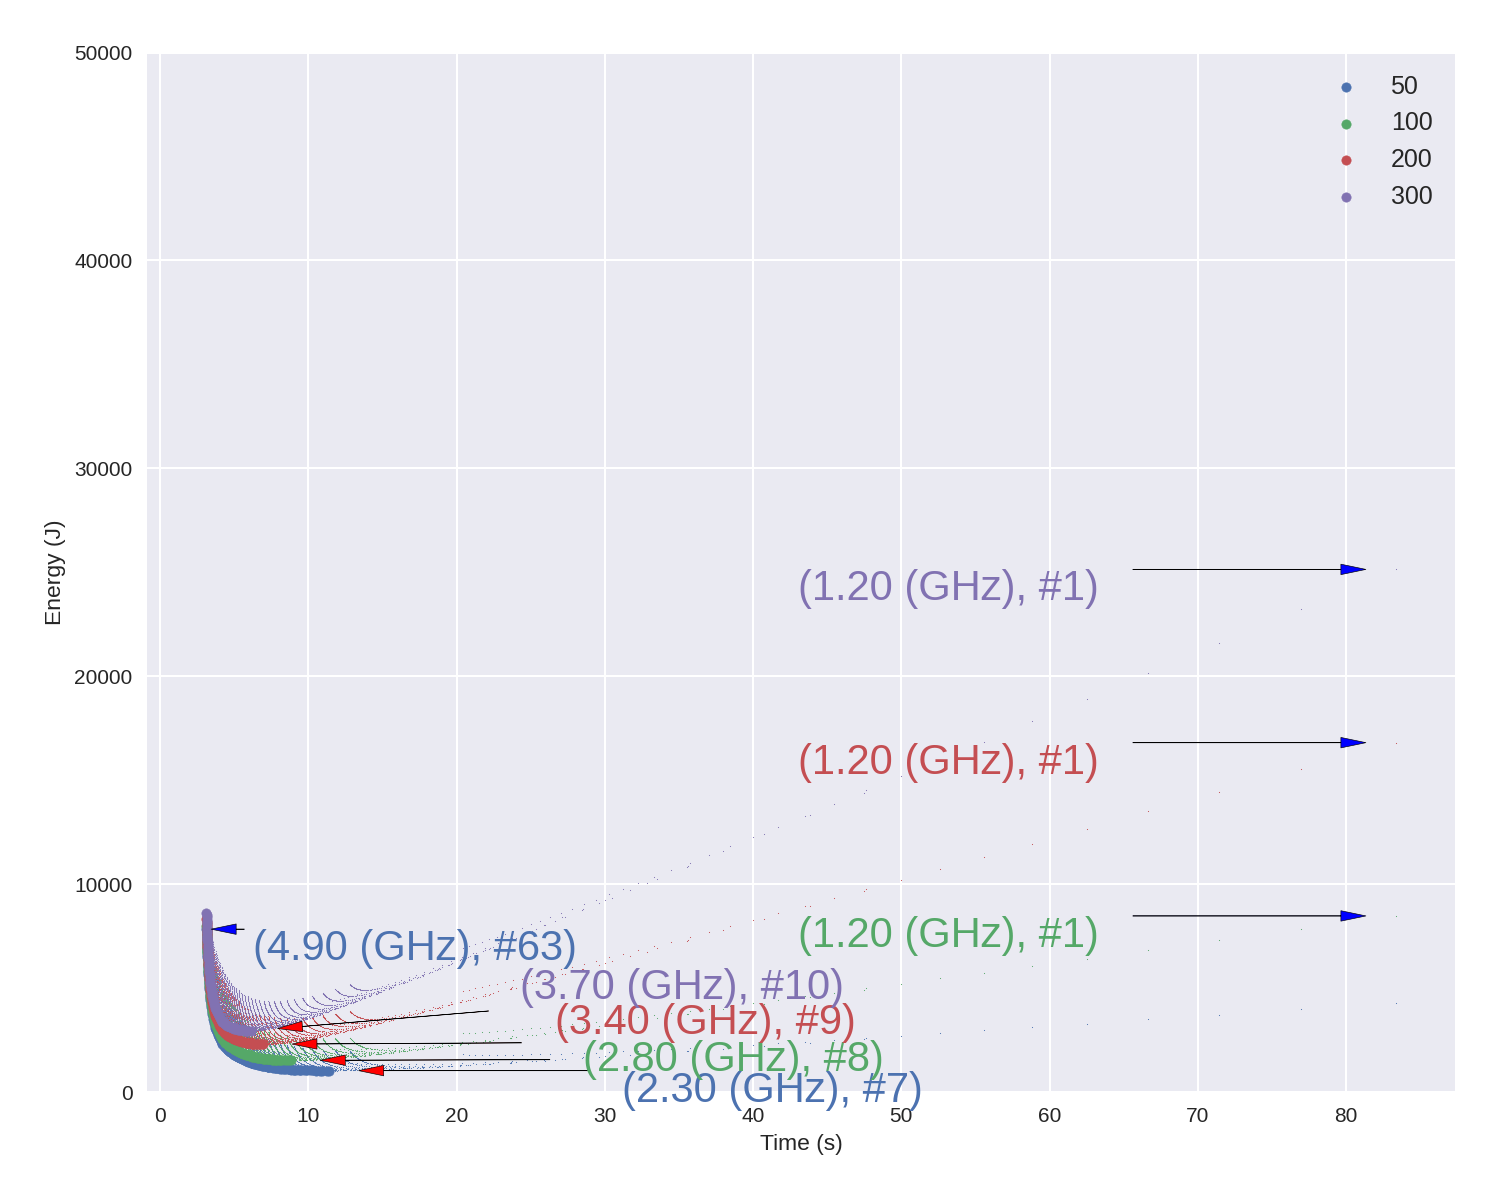
\includegraphics[width=\columnwidth]{models/figures/analisys/pareto_static_high.png}
	\caption{Pareto static energy}
	\label{fig:pareto_static_h}
\end{figure}


\begin{figure}
	\centering
	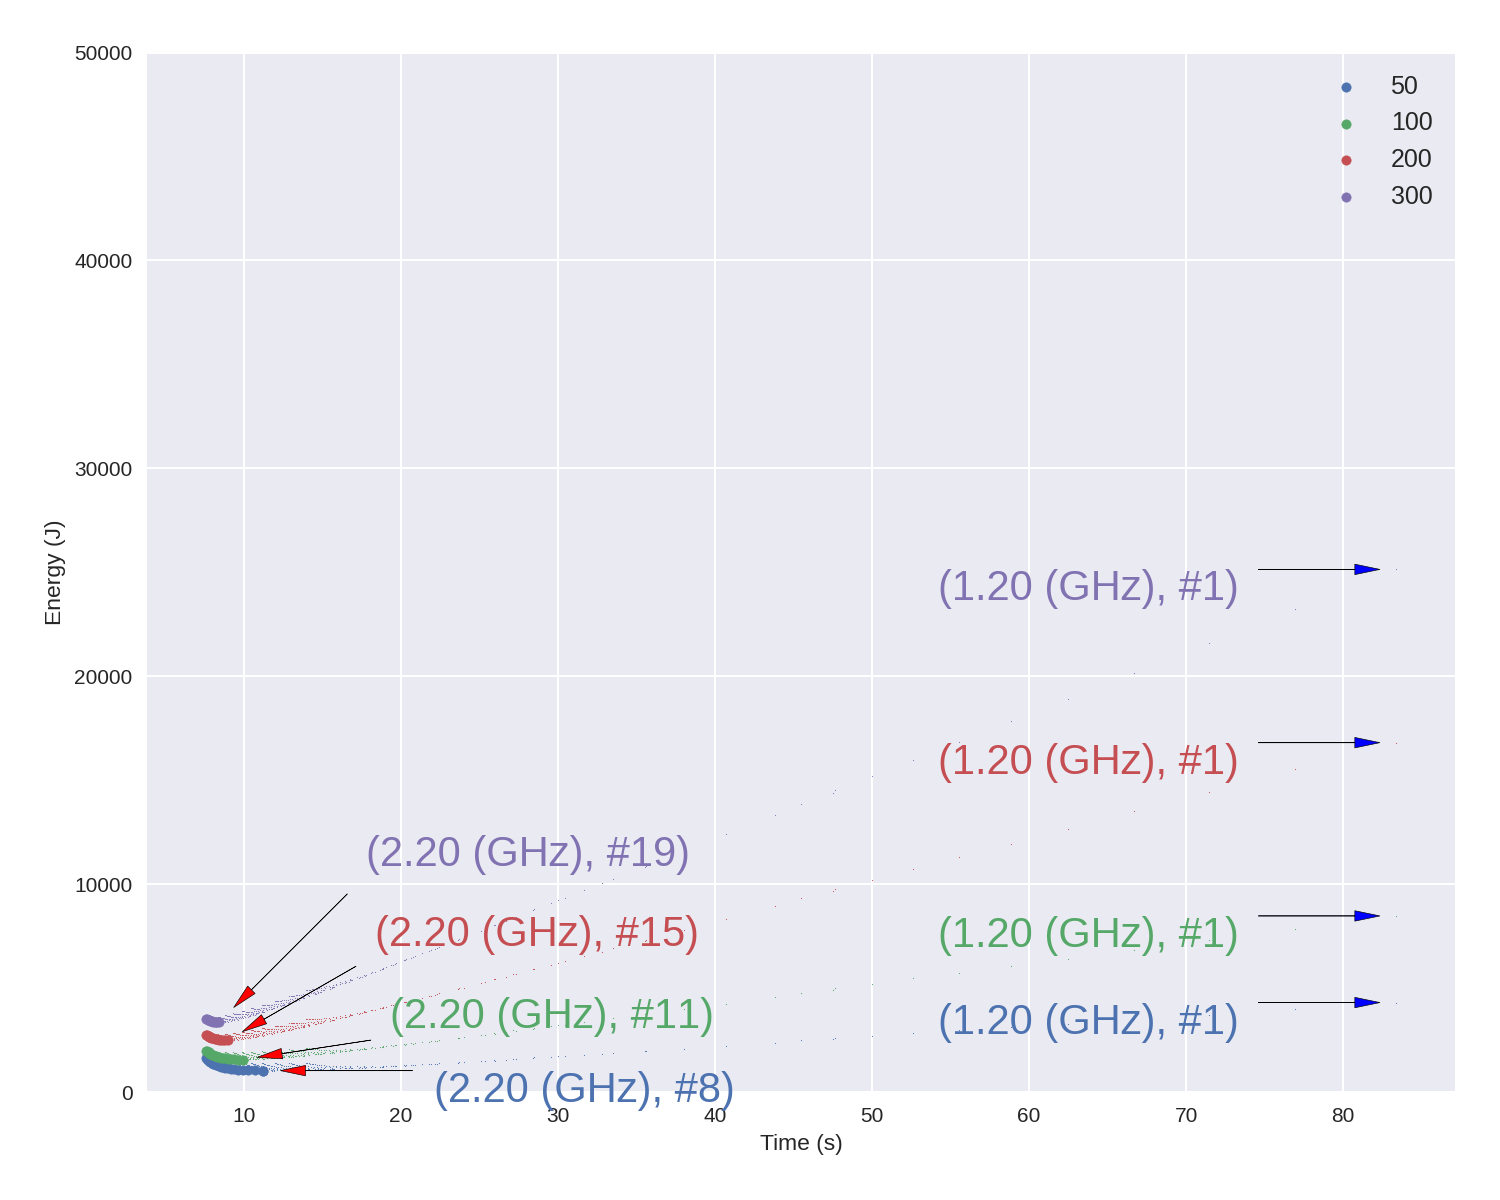
\includegraphics[width=\columnwidth]{models/figures/analisys/pareto_static_low.png}
	\caption{Pareto static energy}
	\label{fig:pareto_static_l}
\end{figure}


\begin{figure}
	\centering
	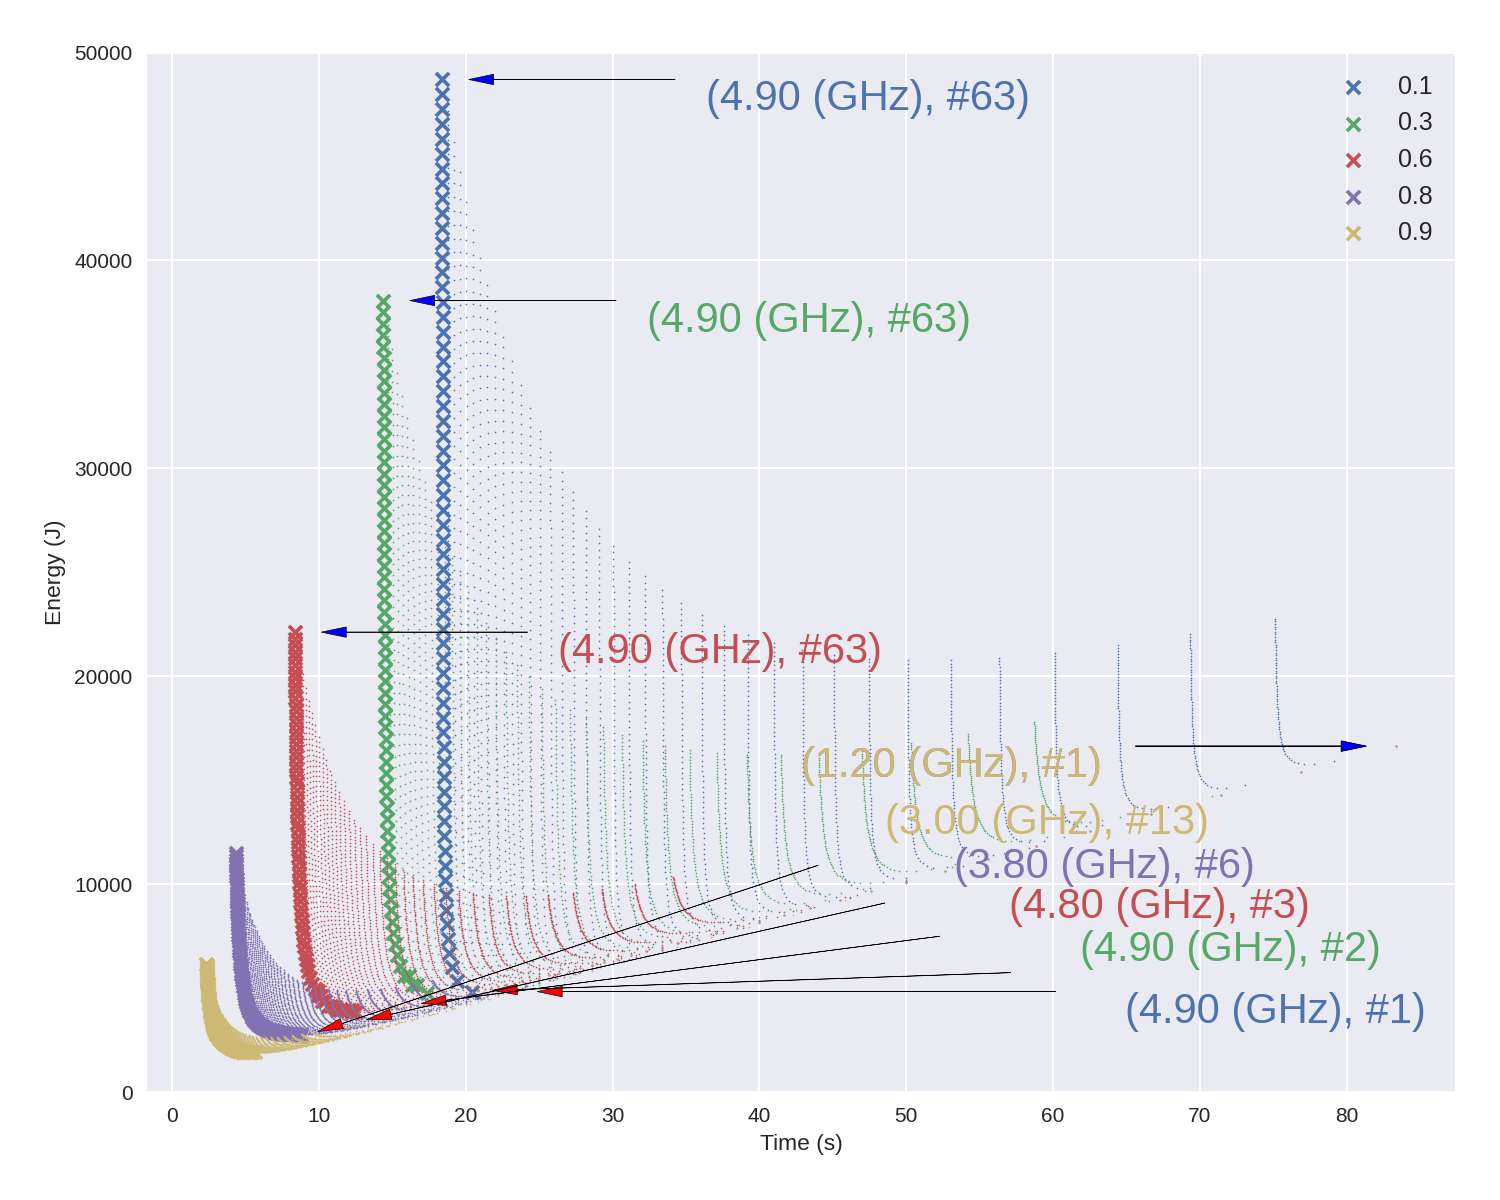
\includegraphics[width=\columnwidth]{models/figures/analisys/pareto_w_high.png}
	\caption{Pareto w energy}
	\label{fig:pareto_w_h}
\end{figure}

\begin{figure}
	\centering
	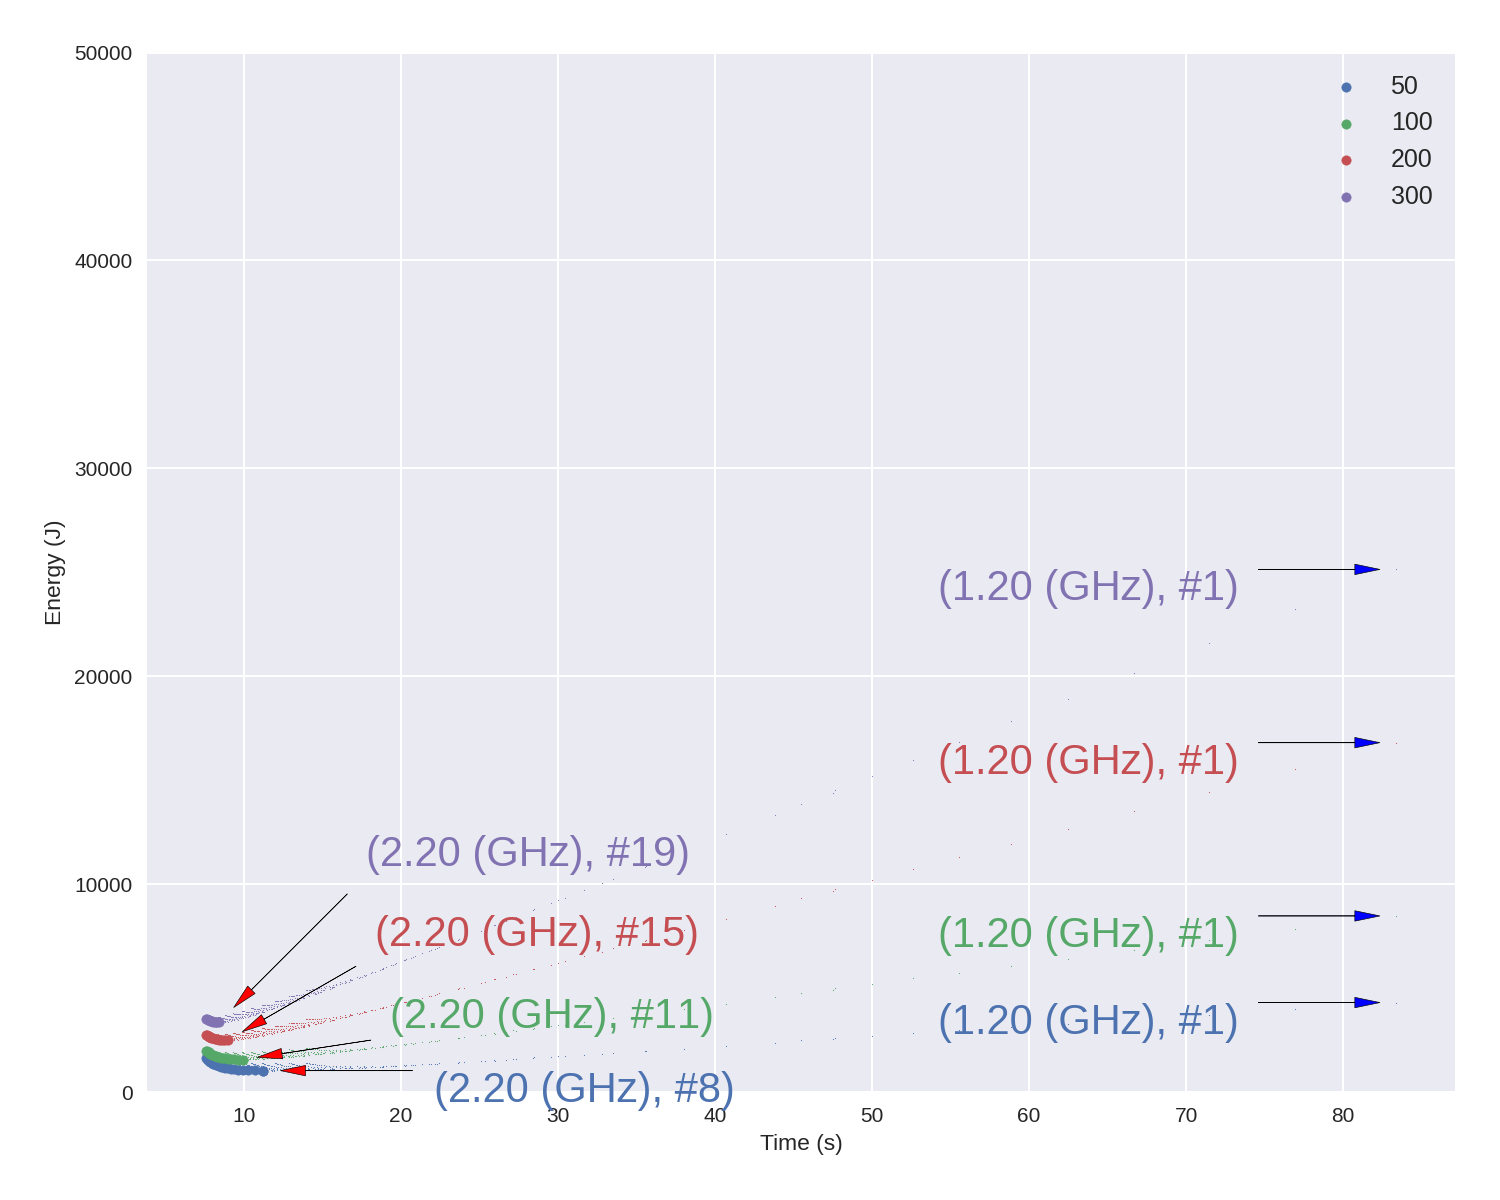
\includegraphics[width=\columnwidth]{models/figures/analisys/pareto_static_low.png}
	\caption{Pareto w energy}
	\label{fig:pareto_w_l}
\end{figure}

\subsection{Optimization under constraints}

\subsection{Gradient}

\begin{figure}[H]
	\centering
	\begin{subfigure}[b]{0.45\textwidth}
		\includegraphics[width=\textwidth]{ch5/image182}
	\end{subfigure}
	%
	\begin{subfigure}[b]{0.45\textwidth}
		\includegraphics[width=\textwidth]{ch5/image181}
	\end{subfigure}
\end{figure}

\begin{figure}[H]
	\centering
	\begin{subfigure}[b]{0.45\textwidth}
		\includegraphics[width=\textwidth]{ch5/image184}
	\end{subfigure}
	%
	\begin{subfigure}[b]{0.45\textwidth}
		\includegraphics[width=\textwidth]{ch5/image183}
	\end{subfigure}
\end{figure}

\begin{figure}[H]
	\centering
	\begin{subfigure}[b]{0.45\textwidth}
		\includegraphics[width=\textwidth]{ch5/image186}
	\end{subfigure}
	%
	\begin{subfigure}[b]{0.45\textwidth}
		\includegraphics[width=\textwidth]{ch5/image185}
	\end{subfigure}
\end{figure}

\begin{figure}[H]
	\centering
	\begin{subfigure}[b]{0.45\textwidth}
		\includegraphics[width=\textwidth]{ch5/image188}
	\end{subfigure}
	%
	\begin{subfigure}[b]{0.45\textwidth}
		\includegraphics[width=\textwidth]{ch5/image187}
	\end{subfigure}
\end{figure}

\begin{figure}[H]
	\centering
	\begin{subfigure}[b]{0.45\textwidth}
		\includegraphics[width=\textwidth]{ch5/image198}
	\end{subfigure}
	%
	\begin{subfigure}[b]{0.45\textwidth}
		\includegraphics[width=\textwidth]{ch5/image197}
	\end{subfigure}
\end{figure}

\begin{figure}[H]
	\centering
	\begin{subfigure}[b]{0.45\textwidth}
		\includegraphics[width=\textwidth]{ch5/image200}
	\end{subfigure}
	%
	\begin{subfigure}[b]{0.45\textwidth}
		\includegraphics[width=\textwidth]{ch5/image199}
	\end{subfigure}
\end{figure}

\begin{figure}[H]
	\centering
	\begin{subfigure}[b]{0.45\textwidth}
		\includegraphics[width=\textwidth]{ch5/image202}
	\end{subfigure}
	%
	\begin{subfigure}[b]{0.45\textwidth}
		\includegraphics[width=\textwidth]{ch5/image201}
	\end{subfigure}
\end{figure}

\begin{figure}[H]
	\centering
	\begin{subfigure}[b]{0.45\textwidth}
		\includegraphics[width=\textwidth]{ch5/image204}
	\end{subfigure}
	%
	\begin{subfigure}[b]{0.45\textwidth}
		\includegraphics[width=\textwidth]{ch5/image203}
	\end{subfigure}
\end{figure}


\subsection{Countorns}

\begin{figure}[H]
	\centering
	\begin{subfigure}[b]{0.45\textwidth}
		\includegraphics[width=\textwidth]{ch5/image202}
	\end{subfigure}
	%
	\begin{subfigure}[b]{0.45\textwidth}
		\includegraphics[width=\textwidth]{ch5/image208}
	\end{subfigure}
\end{figure}

\begin{figure}[H]
	\centering
	\begin{subfigure}[b]{0.45\textwidth}
		\includegraphics[width=\textwidth]{ch5/image204}
	\end{subfigure}
	%
	\begin{subfigure}[b]{0.45\textwidth}
		\includegraphics[width=\textwidth]{ch5/image206}
	\end{subfigure}
\end{figure}

\begin{figure}[H]
	\centering
	\begin{subfigure}[b]{0.45\textwidth}
		\includegraphics[width=\textwidth]{ch5/image198}
	\end{subfigure}
	%
	\begin{subfigure}[b]{0.45\textwidth}
		\includegraphics[width=\textwidth]{ch5/image211}
	\end{subfigure}
\end{figure}

\begin{figure}[H]
	\centering
	\begin{subfigure}[b]{0.45\textwidth}
		\includegraphics[width=\textwidth]{ch5/image200}
	\end{subfigure}
	%
	\begin{subfigure}[b]{0.45\textwidth}
		\includegraphics[width=\textwidth]{ch5/image212}
	\end{subfigure}
\end{figure}

\begin{figure}[H]
	\centering
	\begin{subfigure}[b]{0.45\textwidth}
		\includegraphics[width=\textwidth]{ch5/image186}
	\end{subfigure}
	%
	\begin{subfigure}[b]{0.45\textwidth}
		\includegraphics[width=\textwidth]{ch5/image217}
	\end{subfigure}
\end{figure}

\begin{figure}[H]
	\centering
	\begin{subfigure}[b]{0.45\textwidth}
		\includegraphics[width=\textwidth]{ch5/image188}
	\end{subfigure}
	%
	\begin{subfigure}[b]{0.45\textwidth}
		\includegraphics[width=\textwidth]{ch5/image218}
	\end{subfigure}
\end{figure}

\begin{figure}[H]
	\centering
	\begin{subfigure}[b]{0.45\textwidth}
		\includegraphics[width=\textwidth]{ch5/image182}
	\end{subfigure}
	%
	\begin{subfigure}[b]{0.45\textwidth}
		\includegraphics[width=\textwidth]{ch5/image219}
	\end{subfigure}
\end{figure}

\begin{figure}[H]
	\centering
	\begin{subfigure}[b]{0.45\textwidth}
		\includegraphics[width=\textwidth]{ch5/image184}
	\end{subfigure}
	%
	\begin{subfigure}[b]{0.45\textwidth}
		\includegraphics[width=\textwidth]{ch5/image220}
	\end{subfigure}
\end{figure}



\chapter{Optmizers}
This chapter talks about the different types of optimizers.
\section{Common approaches to the optimization problems}

To build the optimization problem it's necessary to model the system power and application, and controllable variables. Common approaches to the optimization problems are:

Minimize the energy function in function of our control variables, subject to constraints in the control variable.

\begin{equation}
\begin{aligned}
\textrm{min} \quad & P(s_1, s_2, ...)T(s_1,s_2,...)\\
\textrm{subject to} \quad & b_1<s_1<b_2\\
\quad & b_3<s_2<b_4\\
\quad & \vdots\\
\end{aligned}
\end{equation}

Another way is to minimize the total energy, with the constraint of to finish the work.

\begin{equation}
\begin{aligned}
\textrm{min} \quad & \sum{P_it_i}\\
\textrm{subject to} \quad & W_{tot} = \sum w_i\\
\quad & \vdots\\
\end{aligned}
\end{equation}

This kind of problem can be seen in multiple ways, considering an application as the total workload and choosing different speeds for each phase of the application, or could also treat each workload as a different application and create schedulers both CPU and cluster level. In fact the question of on each level of optimizer produces a better result is not well explored in the literature yet. The habitual approach it's to tackle each problem at once and combine the strategies resulting in a chain of schedulers.

The complexity of this problem also varies, depending on the choice of power function it can result in linear programming \cite{Kim2015RacingHeuristics}, quadratic programming \cite{Horyath2008Multi-modeClusters}, until NP-hard problems \cite{Fu2018RaceMinimization}.

\subsection{DVFS optimization} \label{sec:dvfs_optmin}
The effectiveness of the proposed approach for optimization was evaluated with a simple algorithm that finds the optimal frequency and number of active cores from the equation proposed. The results were then compared to the Linux default choices for power management.

With the equation developed \ref{eq:en_final}, it is possible to calculate energy consumption estimations for every possible configuration since there is a finite interval of possible values for the frequency and cores. Then, the configuration that minimizes energy consumption for a given input can be selected. It is also possible to apply constraints on the execution time, frequency, and the number of active cores.

Current HPC managers leave to the user the choice of how many cores to use. Because of that three situations were analyzed with relation to the number of cores:

\begin{enumerate}
	\item Worst choice: number of cores that maximize the total energy consumed
	\item Random choice: energy consumed for a random choice of number of cores
	\item Best choice: number of cores that minimize the total energy consumed (oracle)
\end{enumerate}

The default option for the Linux governor is the Ondemand, and by default, it does not have a DPM control for the number of active cores. Since Ondemand only does DVFS, to allow the comparison, each application was executed with all number of cores available in the system 1 to 32.

Figures \ref{fig:energy_worst_case}, \ref{fig:energy_mean_case} and \ref{fig:energy_best_case}, shows the energy savings with respect to Ondemand in the following way $\frac{Ondemand-Model_{min}}{Ondemand}$ with all three cases described above. The list below shows the savings and losses for each case:


\begin{figure}[ht]
	\centering
	\includegraphics[width=\columnwidth,height=8.5cm]{models/figures/dvfs_cmp_max.png}
	\caption{Energy saving comparison with the proposed model and for the worst case}
	\label{fig:energy_worst_case}
\end{figure}

\begin{figure}[H]
	\centering
	\includegraphics[width=\columnwidth]{models/figures/dvfs_cmp_mean.png}
	\caption{Energy saving comparison with the proposed model and for the random case}
	\label{fig:energy_mean_case}
\end{figure}

\begin{figure}[H]
	\centering
	\includegraphics[width=\columnwidth]{models/figures/dvfs_cmp_32.png}
	\caption{Energy saving comparison with the proposed model and for the best case}
	\label{fig:energy_best_case}
\end{figure}

The list below shows the savings and losses for each case:

\begin{enumerate}
	\item Worst choice: save 69.88\% on average
	\item Random choice: save 12.04\% on average
	\item Best choice: lost 14.06\% on average
\end{enumerate}

%This can be explained by the linear speedup characteristic from this application. Thus, it is to be expected that on constant efficiency, the better solution will be with more cores.

%The other results on the other applications show that the proposed approach, even in cases on the bests configurations for DVFS, demonstrate that can obtain energy saving of up 18\%, comparing to the Ondemand governor.

%\begin{figure}[H]
%    \centering
%    \includegraphics[width=\columnwidth]{dvfs/completo_black_ondemand_nolimit_2_10.png}
%    \caption{Caption}
%    \label{fig:my_label}
%\end{figure}
%
%In general, for the case-study applications and case-study architecture, the optimal-energy configurations tend to be the ones using the highest frequency, which characterizes a race-to-idle rather than a pace-to-idle optimal behavior~\cite{Kim2015RacingHeuristics}. This can be explained by the large static power observed in the considered architecture, evidenced by the large $c_3$ parameter in (\ref{eq_power_final}) that was fitted in (\ref{eq:fittedpower}). With a large static power, using a pace-to-idle strategy, i.e. the use of frequencies lower than the maximum, is expected to be effective only if the sum of the leakage and the dynamic power parcels is larger than the static power parcel. 
%Based on the fitted power model, this would never happen, i.e. the sum of leakage and dynamic power is always less than the static power,
%\begin{equation*}
%p(0.29f^3+0.97f)+9.18s < 198.59, 
%\end{equation*}
%even if we use the maximum number of cores, $p=32$ and $s=2$, and the maximum frequency, $f=2.2$.
%Nevertheless, race-to-idle was not always the best strategy because energy scales with the execution time, which in turn scales inversely with the number of active cores and the operating frequency, and because power scales linearly with the number of cores, but exponentially with the frequency.
%
%The optimal number of active cores depends on the parallel scalability of the application. The more scalable the application, the more cores it requires to minimize energy. A scalable application can increasingly exchange the speedup of more cores with lower frequencies in order to spend less energy. This is because of the linear relationship between power and number of cores and the exponential relationship between power and frequency.
%
%In all cases, the method proposed here outperformed the worst case of the Ondemand governor. On average, the difference in energy consumption was about 790\%, being 1298\% the maximum difference and 59\% the minimum. In general, the energy consumption of the DFVS scheme was larger for smaller numbers of cores. Nonetheless, it was not always the case that the best number of cores for this scheme was the maximum, i.e. 32 cores. Possibly, for architectures with larger number of cores, choosing the exact number the minimizes energy consumption would be less evident.

Since the number of cores in HPC is requested by the user, the number of CPU requests during one year in UFRN's cluster was analyzed. The result is plotted in the figure \ref{fig:cpu_requests}.
\begin{figure}[H]
	\centering
	\includegraphics[width=\columnwidth]{models/figures/cpu_request.png}
	\caption{Number of CPUs requested by the users during 2016-2017}
	\label{fig:cpu_requests}
\end{figure}

The worst choice was always with a single core and is the most common choice of many regular users. The best choice was quite often 32 cores, which is the third most popular choice of the users but it is $72\times$ less than 1 core. This can point a direction of how much energy can be saved by using this technique for DPM or more advanced optimization algorithms that can be derived from our model.

In practice, this approach can be brought into production by allowing the resource manager to perform these changes for the user using pre-scripts and post-scripts for job submissions with energy consumption requirements. This approach is simple to be implemented and can work in almost any Linux system.


\section{Conclusion} \label{sec:conclusion}
This work proposes an energy model based on the frequency and number of cores for a full shared memory system. This model can serve as a base for DVFS and DPM optimization problems that include both frequency and active cores, as well for analysis of the contribution of each parameter (ex: parallelism level) to the energy consumption.

Results from 3 HPC benchmarks running in one cluster demonstrate the potential of the proposed novel model. While consuming less energy than traditional machine learning approaches, it can serve as bases from DVFS and DPM algorithm as shown in the \ref{sec:dvfs_optmin} in an average case saving about 12\% up to 69\%. The previous knowledge of the application's performance can expose sufficiently relevant information, such as parallel speedups, that is harder to guess in run-time techniques based on DVFS.

A weakness of the proposed model is the need for information about the input size of the application that can be complex to derive. A possible solution would be to precisely define what is input size, given an definition in function of common variable for all applications like throughput for example. Future work will demonstrate all the possible analysis that is possible to archive with the equation as long as more advanced DVFS models that can be derived using the equation. For instance identification of different phases of the target program and thus, it will enable more fine-grained changes of the frequency and, perhaps, the number of active cores, to further improve the results presented here.

Another important aspect that is typically not taken into account is the number of processing cores to be used by a parallel program. This choice is left to the user, which often is not trivial as shown in this paper.


%%%% moved to the conclusions.
% A weak of this approach is that the model of performance and power needed to be trained with previously known input sizes. This weakness can be treated with a future solution that can incorporate a prediction of input size during execution of the application. 



\chapter{Framework}
This chapter introduces the framework developed, the fingerprint tool and pascal analyzer.
\section{Profiling with performance counters} \label{sec:profiling_with_performance_counters}
The analysis of application performance is essential to better exploit its potential on High-Performance Computing (HPC) architectures. Access to performance counters, available in modern processors, allows collecting key information about program behavior to provide the most appropriate HPC execution strategy.
In this context, we have developed an accurate tool based on performance counters, which facilitates modeling, fingerprinting, behavior comparison and clustering of applications.
It provides a high-level Python API for accessing and configuring performance counters; while execution and counters data gathering is  performed by a C++ module to reduce overhead. 
Indeed, the accuracy of this multiplatform tool was also compared to existing alternatives.  
Key features, such as performance counters collection, post-processing, and comparison, enable fingerprinting of applications, an important step in understanding program behavior for later classification and optimization according to the parameters characterizing the target HPC platform.
For demonstration purposes, the tool was used in the clustering of Polybench applications, a frequently used benchmark set for kernels monitoring. 
%%, a frequently used benchmark for compiler optimization and testing. 
This clustering facilitated the identification of applications with similar and comparable behaviors in terms of input size, data access and transfer, resource utilization and computation, which facilitates the creation of test sets for a given environment based on specific measurement parameters.


%%%%%%%%%%%%%%%%%%%%%%%%%%%%%%%%%%%%%%%%%%%%%%%%%%%%%%%%%%%%%%%%%%%%%%%%%%%%%%%%
\section{Collecting performance counters} \label{sec:collecting_performance_countersl}

Hardware Performance Counters are special registers available on most modern processors capable of counting micro-architectural events such as instructions executed, cache-hit, branches miss-predicted, energy estimation and much more.  In new architectures, there are hundreds of hardware events that can be monitored, and more are added to each new generation. 
Performance counters were initially introduced for debugging, but since then they have provided a lot of useful information about running applications without slowing down the execution.
They have been used in several other areas, such as software profiling \cite{Melo2010Perf, Kufrin2005Perfsuite, Knupfer2011Scorep}, CPU power modeling \cite{Zamani2012ASystems}, dynamic frequency and voltage scaling, vulnerability research and malware defense \cite{Demme2013OnCounters}.

%\cite{Geimer2010, Geimer2010TheArchitecture, Shende2006TheSystem}

Exploiting Performance Monitoring Units (PMU) requires an intimate knowledge of the micro-architecture and kernel API, as well as an awareness of an ever increasing complexity. 
Otherwise, the measurement performance and accuracy will be seriously affected. Although many tools have been developed using performance counters, programmable interfaces capable of providing good accuracy are still lacking, especially for high-level programming languages. Indeed, apart from PAPI \cite{Weaver2013Non-determinismImplementations, Mucci1999PAPI} and Perfmon \cite{Eranian2008Perfmon2} there are only a few APIs allowing access to these counters, and many others are poorly documented, unstable, or designer for a specific purpose.

Performance metrics may have different definitions and programming interfaces on different platforms. 
Therefore, besides gathering information, post-processing modules are also needed. 
Such modules will overcome the lack of precision of counters on some architectures, as indicated in \cite{Weaver2008CanTrusted,Weaver2013Non-determinismImplementations,Das2019SoK:Security}. 
Events that must be precise and deterministic (such as retired instructions) show a variation on run-to-run and over-count on x86\_64 machines, even in strictly controlled environments. These effects are almost always non-intuitive to casual users and pose problems when strict determinism is desirable. 

To meet the above mentioned requirements, our strategy combines low-level, efficient and accurate access to PMUs, facilitated by high-level programmable interfaces. This allows the user to perform all configurations and post-processing in Python,  while the underlined architecture details and information gathering are supported by a C++ module, thus preserving accuracy with limited overhead. 
In order to understand the behavior of programs for future comparisons and classification, the proposed tool makes another contribution: the ability to fingerprint and cluster applications.

The definition of reference parameters, such as input size of programs, and performance measures uniformization, allow us to cluster benchmarks such as PolyBench \cite{Gonzalez2021PolyBench}, a collection of numerical computations with static control flow extracted from various application domains, with interesting results. 
In addition to contributing to the standardization of kernel execution and monitoring, this clustering has identified applications with similar and comparable behavior in terms of input size, data transfer and access, resources used and computation; which facilitates the creation of test sets for a given environment, according to specific measurement parameters. 

The rest of this article is organized as follows. subsection 2 provides the related work regarding tools available and requirements. subsection 3 presents the performance counters and motivation. subsection 4 presents our clustering and application analysis tool, architecture and components. subsection 5 shows evaluation results: the comparison of existing API and the clustering of the PolyBench benchmarks. Finally, subsection 8 concludes this article.

\section{State of the art performance counters APIs} \label{sec:state_of_the_art_performance_counters_APIs}

There are only a few APIs allowing access to performance counters.
PAPI \cite{Weaver2013Non-determinismImplementations, Mucci1999PAPI}, one of the most used libraries for accessing hardware performance counters, was originally developed to provide portable access to the counters found on a diverse collection of modern microprocessors. Rather than learning and writing a new performance infrastructure every time it is ported to a new machine. Measurement code can be written in the PAPI API, which hides the underlying interface.  
PAPI was developed on C and a few non-official libraries were ported to Python. The main problem we found using PAPI was the Python version of has a considerable overhead, it also does not have an easy way to create raw events or low-level control without having to use a special driver. And as our tests will show later, counters sampling over time does not produce good results either.

There are also available a set of interfaces using their own drivers, mainly because the counters are only accessible in kernel mode (ring 0) to control the events for which the counter must be started or stopped. Some events are fixed and others require the development of a dedicated kernel driver. 

Perfctr \cite{Nikolaev2011Perfctr} supports per-kernel-thread and system-wide monitoring for most major processor architectures. It is distributed as a stand-alone kernel patch. The interface is mostly used by tools built on top of the PAPI performance toolkit. 

The Intel VTUNE \cite{Intel2021Vtune} performance analyzer comes with its own kernel interface, implemented by an open-source driver. The interface supports system-wide monitoring only and is very specific to the needs of the tool.

The problem with the approach of a tool and its own kernel interface is dangerous because, as mentioned on \cite{Eranian2008Perfmon2}, there is clearly code duplication, but more importantly, there is no coordination between the various interfaces that may coexist sharing access to the same PMU resource. To solve this problem, Perfmon2 \cite{Eranian2008Perfmon2} offers a standard interface that all tools can use. Unfortunately, it has not been widely adopted, just supported by a few architectures like the IA64. Instead, Linux comes up with a performance counters subsystem which provides a complete set of configurations.


\section{Accounting for errors and limitations} \label{sec:accounting_for_errors_and_limitations}

Although hundreds of events are available for monitoring, only a limited number of counters can be used simultaneously.
Therefore, the events to be monitored should be carefully selected and configured using the available counters.

The number of counters available varies between processor architectures, e.g., modern Intel CPUs \cite{Intel2013IntelGuide} support three fixed and four programmable counters per core. Fixed counters monitor events such as Instruction Retired (how many instructions were completely executed), logical cycles, and reference cycles, while programmable counters can be configured to monitor architectural and non-architectural events. 
However, if additional counters are needed, the available ones must be multiplexed.
The configuration of the counters is done by writing in Model-Specific Registers (MSR), only accessible in ring 0 (kernel mode) as indicated previously. 


% \begin{itemize}
%     \item rdmsr - Reads the contents of a 64-bit model specific register (MSR) specified in the ECX register into registers EDX:EAX. This instruction must be executed at privilege level 0 or in real-address mode
%     \item rdpmc - Is slightly faster that the equivalent rdmsr instruction. rdpmc can also be configured to allow access to the counters from userspace, without being privileged.
% \end{itemize}

Operating systems provide an abstraction of these hardware capabilities to access counters and MSRs. 
On the Linux system, where our work was developed, there is a performance monitoring subsystem which provides per-task and per CPU counters, counter groups, and related event features. 
All events are seen as 64-bit virtual counters, regardless of the width of the underlying hardware counters. 
They are accessible via special file descriptors, one file descriptor per virtual counter, opened via the perf\_event\_open() system call.  %These system call do not use rdpmc, but rdpmc is not necessarily faster than other methods of reading event values.
Counter events can be processed by interrupt, polling or on time. The interrupt operates by hooking a user-defined function to a specified event, such as a counter overflow, and whenever this event happens, a signal will be generated passing the control to the designated handler function. With polling, whenever an event occurs on the system, the counter value is queued by the operating system and the user can read from this queue using a system call. The last option is to sample over time reading counters every n second.

Ideal hardware performance counters provide exact deterministic results. Real-world PMU implementations do not always live up to this ideal \cite{Weaver2008CanTrusted, Weaver2013Non-determinismImplementations, Das2019SoK:Security, McGuire2009AnalysisKernel}. Events that should be exact and deterministic (such as the number of executed instructions) show run-to-run variations and over counts on x86 64 machines, even when running in strictly controlled environments. 
These effects are non-intuitive to casual users and cause difficulties when strict determinism is desirable, such as when implementing deterministic replay or deterministic threading libraries. 
Because of that, we have implemented a methodology to reduce the noise and over counts on performance counters.


\section{Implementing a tool to read performance counters precisely} \label{sec:implementing_a_tool_to_read_performance_counters_precisely}

%This module provide a high-level abstraction API to Linux perf events without overhead while executing

This tool is composed of 5 modules the are Profiler, Events, Workload, Analyzer and libpfm4. 
The Workload and libpfm4 module are developed on C/C++ and interfaced with python using Python C API with SWIG (a software development tool to connects programs written in C/C++ with a variety of high-level programming languages). 
The libpfm4 module, developed by \cite{Eranian2008Perfmon2}, is used as an auxiliary library.

%The main features that this library provide is a precise synchronous start the application and counter the event, a low overhead on sampling the events on time and an easy way to find and configure event in groups or standalone. 

\section{PMC tool architecture} \label{sec:PMC_tool_architecture}

In figure \ref{fig:achitecture} we can see how these modules interact with each other.
\begin{figure}[H]
    \centering
    \includegraphics[width=\textwidth]{fingerprint/figures/architecture.png}
    \caption{Modules interconnection}
    \label{fig:achitecture}
\end{figure}

The Profiler is the user interface for configuring and creating events.
It is also responsible for calling the Workload module to run the application and retrieve the data after the execution is complete.

The Workload module, developed on C++, is the core of the library.
It is responsible for creating the application and the sampling process.
It provides a precisely synchronized start, it halts the program before the execution of the first instruction, using the debug interface on Linux (place), and launches the application once the counters have been properly reset and ready to run.
This module, built-in as a Python module using the Python C API, defines a set of functions, macros, and variables to access most aspects of the Python run-time system.
% The workload run simplified code
% \begin{lstlisting}[language=c++]
% reset_counters();
% start_counters();
% start_application();
% while(application.is_running()){
%      sleep(secounds);
%      sample_counters();
% }
% return sampled data;
% \end{lstlisting}
The Event module provides a description of events, events parameters, configurations and PMUs available.

System calls for reading and event creation are done directly by the Workload module or through the libpfm4 Python link. 
The libpfm4 is also used to find events encodings and convert an event name (expressed as a string) to the corresponding event encoding, either as a raw event number (as documented by the hardware vendor) or the OS-specific encoding.
In the latter case, the library is able to prepare the OS-specific data structures needed by the kernel to setup the event.

The Analyzer module is responsible for the post-processing of the data. 
It takes the data from several runs of the application and provides a set of functions to remove outlines, interpolate, filter and compare.
% \subsubsection{FUNCTIONALITY}
% This subsection is going to describe the main functionality of the API.
% Profiler module:
% \begin{lstlisting}[language=Python]
% Profiler(events_groups, program_args=None)
% \end{lstlisting}
% This constructor creates a profiler object from a list of events groups with their names, optionally can pass the application that will be executed.
% \\
% \begin{lstlisting}[language=Python]
% set_program(program_args)
% \end{lstlisting}
% Set the program and his arguments to be executed from a list.
% \\
% \begin{lstlisting}[language=Python]
% start_counters(pid=0)
% \end{lstlisting}
% Monitor events by pid. If pid its set to 0, monitor the entire system.
% \\
% \begin{lstlisting}[language=Python]
% enable_events()
% disable_events()
% reset_events()
% read_events()
% \end{lstlisting}
% Control events
% \\
% \begin{lstlisting}[language=Python]
% run(sample_period, reset_on_sample=False)
% \end{lstlisting}
% Run the application and sample the events on the time, it receives the sample time and if a flat that controls the reset on the sample. It returns the data with the events sampled. 
% \\
% \begin{lstlisting}[language=Python]
% run_background()
% \end{lstlisting}
% Run the application in background
% \begin{lstlisting}[language=Python]
% run_program(...)
% save_data(data, name)
% \end{lstlisting}
% Simple functions to run a program multiple times and store the results in a file.
% \\
% \\
% Events module:
% \begin{lstlisting}[language=Python]
% get_supported_pmus()
% get_supported_events(name)
% get_event_description(name)
% get_event_attrs(name)
% \end{lstlisting}
% These functions return a list with a description for the PMU, event, and attributes.
% \\
% \\
% Analyser module:
% \begin{lstlisting}[language=Python]
% load_data(name)
% \end{lstlisting}
% Load the data capture into an Analyser object.
% \\
% \begin{lstlisting}[language=Python]
% process(verbose=False)
% \end{lstlisting}
% Process the data, using the method described on the post-processing subsection \ref{sec:posprocessing}.
% \\
% \begin{lstlisting}[language=Python]
% compare(a1, a2, feature, npoints)
% \end{lstlisting}
% Compare two objects on a specific feature.

\section{Post-processing} \label{sec:posprocessing}
% With this API we create clusterize the applications of Polybench applications.

With the data collected from multiple runs of the application, the first goal is to obtain a single curve that minimizes the noise caused by the operating system and inaccuracies of the counters. 
In figure \ref{fig:multiple_exec} we can see the raw result of multiple runs of the Polybench 2mm program measuring the number of executed instructions. 
For better visualization, the horizontal axis has been normalized over the interval from 0 to 100. 
This implies that we no longer analyze the program on the time scale, but in the interval in which it took place.

\begin{figure}[H]
    \centering
    \includegraphics[width=\textwidth]{fingerprint/figures/workflow.png}
    \caption{Multiple executions of the Polybench 2mm program with different input sizes}
    \label{fig:multiple_exec}
\end{figure}

We apply a median filter to each set of runs, sorting the values and removing edge values.
Then we calculate the average curve, whose final result can be observed on the figure \ref{fig:single_curve}.

\begin{figure}[H]
    \centering
    \includegraphics[width=\textwidth]{fingerprint/figures/workflow_1.png}
    \caption{Single instance representation}
    \label{fig:single_curve}
\end{figure}

 After that, we interpolate the curve using the B-spline \cite{Hang2017CubicApplications} algorithm to get the same number of points to all curves. 
 The result of this step can be observed in figure \ref{fig:interporlation}. 

\begin{figure}[H]
    \centering
    \includegraphics[width=\textwidth]{fingerprint/figures/workflow_2.png}
    \caption{Interpolation}
    \label{fig:interporlation}
\end{figure}

Finally, we use the Savgol filter \cite{Luo2005PropertiesDifferentiators} in order to smooth the data to increase the signal-to-noise ratio without too much distortion. The result is shown in figure \ref{fig:filtering}.

\begin{figure}[H]
    \centering
    \includegraphics[width=\textwidth]{fingerprint/figures/workflow_3.png}
    \caption{Filtering}
    \label{fig:filtering}
\end{figure}






\section{Introduction to profiling tools} \label{sec:introduction_to_profiling_tools}

Developing parallel programs capable of exploiting the computational power of high-performance systems is as well-known as it is challenging~\cite{Huck2007, Islam2019, Weber2019}. 
During the development process, the code optimization step is a fundamental part of the software construction strategy and is supported by performance measurement and analysis tools~\cite{Bergel2019, Weber2019, Huck2005, Geimer2010, Shende2006, Adhianto2010, Miller1995, Galobardes2015, Pillet2007, Islam2019}. The main objective of these tools is to help developers understand the execution characteristics, allowing the identification of bottlenecks and behavioral phenomena that compromise the program’s efficiency, thus guiding possible improvements~\cite{Brink2020, Huck2007}.

Nowadays, due to the complexity of parallel systems, correctly identifying and locating performance and scalability bottlenecks depends on the developer's ability to compare several measurements in different execution configurations~\cite{Bergel2019, Silva2018}. This investigative process tends to be tedious and complex, requiring in-depth knowledge of the problem domain, parallel systems, and measurement and analysis tools.
Mastering the analysis tools is necessary because they differ from each other in terms of measurement strategy, metrics collected, and the many points and focus of observation.
Even though some solutions propose organizing and combining metrics from different sources, these distinct characteristics can compel developers to exploit more than one tool depending on their analysis~interests.

Every existing tool has its own contributions in helping to understand the inner working of a program. Some can present a vast and varied set of metrics with a high degree of detail. 
However, developers may have difficulty using these tools when their interest is in analyzing parallel scalability.
The main challenge arises from the emphasis on studying a single run because scalability analysis requires contrasting runs of different configurations.
In terms of productivity, measuring and comparing only a few data between runs of multiple configurations tends to be more significant to scalability analysis than collecting a vast amount of finer-grain data of single-configuration runs.
Furthermore, due to the number of measurements, there is a natural overhead associated with the execution of the analysis tool itself. Some works indicate this overhead can reach 40\% of the program runtime, which influences and damages the observation of its efficiency variation~\cite{Eriksson2016}.
As such, a measurement and analysis approach that uses only the data needed to understand the application's efficiency variation can be advantageous. First, because measuring and collecting only the necessary data limits the degree of intrusion and, second, because this strategy makes the analysis tool simpler and easier to use. 
~\cite{Shende2006}.


From this context, we present a measurement tool that focuses on analyzing the parallel scalability of programs. It primarily provides runtime and power consumption measures in an approach that favors inspection of the overall behavior of the program before starting a more in-depth investigation of points that naturally require more detail, time and effort.
The work explores and combines strategies already used in other solutions, such as tracing, post-mortem analysis, and automatic instrumentation based on shared libraries. Additionally, it includes an instrumentation model that automatically relates parallel code regions to analysis regions, using a measurement strategy based on the intrinsic and primary behavior of the parallel frameworks. Due to this approach, the tool allows analyzing programs developed for shared-memory environments regardless of the compiler or framework versions. 
The framework version, which in some cases also requires specific compiler versions, is a limitation for some traditional tools like HPCToolkit~\cite{Adhianto2010} and TAU (Tuning and Analysis Utilities)~\cite{Shende2006}.

The proposed tool uses a tracing-based measurement technique to identify and measure the boundaries of the analysis regions. The tracing approach supports a hierarchical region analysis model allowing users to see how the efficiency of inner parts can impact the program's overall scalability. In addition, the tool uses an aggregation feature to reduce the volume of data produced while preserving accurate analysis capability with minimal overhead. The tool also includes usability features that reduce the developer's efforts during the measurement and analysis process. These features allow one to automate the process of running and merging data collected from multiple configurations, bypassing manual efforts and avoiding the drawbacks of non-computer-oriented analysis.
The collected data, available from the terminal in tabular form, can be exported as data blocks that can be interpreted by other tools or even rendered by graphics libraries to facilitate the visualization and data analysis.


We offer an alternative tool for realizing parallel scalability analysis more efficiently than single-run-centric performance measurement and analysis tools. In addition to that, our framework can also be used to promote energy-aware software; methods that rely on accurate and efficient energy collection could benefit from energy consumption data for the entire program and specific regions of the application \cite{10.1007/978-3-319-58667-0_22,10.1007/978-3-319-58667-0_21,7016382,10.1145/3321551}. To summarize, the main contributions of this work are:

\begin{itemize}
	\item A lightweight automated process of measuring and comparing runs with different configurations.
	\item Transparent linking of parallel code sections to analysis regions.
	\item Hierarchical views and degrees of efficiency for the inner parts of a program.
	\item The imposed overhead is low and minimally intrusive, mainly because of the measurement approach and the number of metrics collected.
	\item It provides energy consumption measures for the different configuration parameters. 
\end{itemize}

The following sections describe how the tool is built and used for performance analysis. Section \ref{sec:state_of_the_art_profiling_and_tracing_tools} presents the related works. Section \ref{sec:pascal_architecture} describes the tool architecture and goals; it explains the main features, usage, and collected data. The experimental results are presented in Section \ref{sec:pascal_framework_validation}. Finally, the contributions are summarized in Section \ref{sec:conclusions_pascal}, with an outlook of future works.

\section{State of the art: profiling and tracing tools} \label{sec:state_of_the_art_profiling_and_tracing_tools}

Performance analysis aimed at code optimization is an essential activity for developing parallel applications with scalable performance. For this purpose, performance analysis tools, like Caliper~\cite{Boehme2016}, HPCToolkit~\cite{Adhianto2010}, Scalasca~\cite{Geimer2010}, TAU~\cite{Shende2006}, Vampir~\cite{Weber2019}, and VTune~\cite{Intel2021Vtune}, are useful because they help developers identify where the application uses the available computing resources inefficiently through collecting detailed data of its execution. Such tools differ from each other mainly in terms of data measurement and analysis strategy: tracing or profiling, post-mortem or real-time; individual or comprehensive observation focus; and for providing or not providing visual elements that facilitate the judgment of collected data. Other solutions, like the DASHING framework~\cite{Islam2019} and the HATCHET library~\cite{Brink2020}, allow inspection of performance data from multiple sources. In this case, the goal of DASHING and HATCHET is to provide a more robust data set to support the analysis process.

In the performance analysis process, observing the parallel program's execution as a sequence of events representing significant activities is essential to understand its behavior~\cite{Pantazopoulos1997}. Events are basic units of the analysis process, and the way they are observed influences strategies for collecting performance data. Profiling-based analysis tools collect information from events that occurs in the program execution and commonly operate by statistical sampling using interruptions. These interruptions can be caused, for example, by periodic breaks or hardware events. Interruptions allow checking the system state and the information collected depends on the focus of observation. Profiling-based tools use statistical techniques to describe the program behavior in terms of aggregate performance metrics. They usually ignore the chronology of events, but are known to be useful for identifying, for example, load imbalance, high communication time, or excessive routine calls. Paradyn~\cite{Miller1995}, and Periscope~\cite{Gerndt2010} are tools that adopt this strategy.

On the other hand, tracing-based analysis tools collect performance data from events that occur when the program takes over a particular state. Tracing can provide valuable information about the time dimension of a program, allowing users to check when and where transitions of routines, communications, and specific events occur. This measurement strategy tends to be more invasive and intrusive, generating a larger dataset than the profiling-based approach. Vampir~\cite{Weber2019} and Paraver~\cite{Labarta2005} are examples of this group. Some tools like HPCToolkit~\cite{Adhianto2010}, Scalasca~\cite{Geimer2010}, TAU~\cite{Shende2006} and VTune~\cite{Intel2021Vtune} support both profiling and~tracing.

%In this work we propose tracing to measure the program and identify when parts of its code were executed. 
In this work we propose tracing to identify when parts of a code were executed. 
%To mitigate some of the disadvantages usually related to tracing, the tool implements features such as automatic instrumentation mode and aggregation resource, in addition to adopting an analysis based only on time. 
To mitigate some of the disadvantages related to tracing, in addition to adopting a time-based analysis, the tool implements features such as automatic instrumentation mode and resources aggregation.
%The automatic instrumentation mode makes it possible for users to analyze the program's execution without modifying the compiled code. 
Our automatic instrumentation mode allows users to analyze program execution without modifying the source or the executable.
Although many other analysis tools use the automatic instrumentation mode, this work presents a different way of mapping and measuring the code parts. 
%In our proposal, parallel regions are the main focus of analysis, and there is no limitation on the version of OpenMP used in the development, as in tools such as HPCToolkit~\cite{Adhianto2010} and TAU~\cite{Shende2006}. 
In our proposal, parallel regions are the main focus of analysis. 
%The strategy is efficient in identifying the scalability trend of parts or the whole parallel program in execution.
The strategy is effective enough to identify the scaling trends of parts or of the entire running parallel program.
%Furthermore, collecting only data related to runtime reduces the associated overhead with the measurement process. 
Furthermore, collecting only specific runtime data reduces the overhead associated with the measurement process.
As with other similar tools, such as HPCToolkit~\cite{Adhianto2010} and TAU~\cite{Shende2006}, there is no limitation on the version of OpenMP~used.

Runtime overhead is an attribute associated with the set of additional instructions that are executed to collect the program measurements. The time to perform this ``extra code'' varies in line with the tool and is directly related, in quantity and degree of detail, to the aspects it measures. 
Limiting this overhead is crucial because it can compromise the understanding of program behavior, and divert optimization efforts to less effective points. 
According to some comparative and practical studies in this regard, tests on traditional tools have shown a runtime overhead ranging from 2\% to 40\%~\cite{Eriksson2016}.
%Fundamental to the proposal of this work, the overhead presented by the proposed tool differs according to the program under analysis but can be considered negligible (<1\%) for analyzing scalability trends of parallel applications.
Although different depending on the program analyzed, the overhead resulting from our instrumentation strategy can be considered negligible (less than 1\%) and optimal for analyzing trends in parallel applications.

Several performance analysis tools employ a post-mortem approach. 
%In this kind of approach, the tools collect performance metrics during the program execution, but the data interpretation is carried out only after its execution. 
In this case, the tool performs performance measurements and data collection while the program is running, and then the collected data will be interpreted.
HPCToolkit~\cite{Adhianto2010}, Scalasca~\cite{Geimer2010}, TAU~\cite{Shende2006} and VTune~\cite{Intel2021Vtune} are examples of post-mortem performance analysis tools. 
%Post-mortem performance analysis tools may require the storage of large volumes of performance data, but they are more suitable to provide an overall view of the execution. 
Depending on the type of analysis, these tools may require storing large amounts of data, but they are best suited to provide an overall view of the execution.
%On the other hand, real-time analysis tools enable performance analysis during the execution of the program. 
In contrast, run-time analysis tools perform both operations at run time.
This approach allows detecting waiting states and communication inefficiencies accurately. 
%However, an online analysis environment usually requires the coordinated usage of extra tools, which increases the analysis infrastructure complexity. 
Periscope~\cite{Gerndt2010} and Paradyn~\cite{Miller1995} are examples of tools in this group.
However, run-time analysis generally requires the coordinated action of tools, which increases the structural complexity.
%The need for synchronous initialization, communication between all resources used in the analysis, and the additional load on the network are disadvantages of the real-time approach. 
The need for synchronous initialization and communication between analysis resources as well as their impact on the runtime environment are the drawbacks of this approach.
%In addition, the analysis that depends on data collected at the end of the program's execution, as in the case of scalability analysis, are potentially damaged by the infrastructure overhead and do not, in practice, benefit from characteristics of real-time tools. 
In addition, the analysis, particularly that of scalability, which relies on the data collected at the end of the execution, is potentially degraded by the infrastructure overhead and therefore does not benefit from the characteristics of real-time tools.


\textls[-15]{Energy management solutions can also provide similar features for example GEOPM~\cite{10.1007/978-3-319-58667-0_21},} allows the measurement of time and energy of specific regions. The main advantage that we could not find in any other framework is that our tool can provide specific data of energy consumption of parallel regions in a completely automated way. For example, in GEOPM, it is necessary to instrument the source code to obtain the same result.

%To investigate the scalability trend, it is more important to identify the program's general behavior than its state at a given moment of execution. 
%Although the current performance analysis tools are helpful and allow to identify numerous aspects regarding the program's behavior, none of them presents characteristics directly focused on observing the scalability trend of parallel code. An indispensable feature for this purpose includes automating the program's measurement process in different configurations because a more accurate understanding of scalability requires measuring and comparing multiple code runs.
%Focused on more practical and objective analysis, we propose an alternative tool to observing a parallel program's scalability trend. It collects only information that allows deriving the overall program runtime, or parts of it, according to the user's interest, and includes relevant functionalities to an efficient measurement and analysis process. Among the supported features it provides: the automation of program runs based on different parameters; the generation of data sets that contain metrics with different execution parameters; and the reduction of the generated data volume on disk.

%Although the current performance analysis tools are helpful and allow to identify numerous aspects regarding the program status, to investigate scalability trends, it is more important to identify the behavior of parallel code rather than its state at a given moment of the execution, therefore the post-mortem approach is more suitable. 
By focusing on objective analysis, we offer an alternative tool to observe the scalability trend of a parallel program. Thus, we collect just the information allowing us to infer the overall behavior of the program, or, according to the interest of the user, specifically chosen parts of it, including features relevant to an effective measurement and analysis process. 
To this end, it is essential to also automate the processes to obtain comparative measurements of several runs. 
Supported features are the automation of program executions according to various configuration parameters, including a user-specified granularity, the generation of datasets containing comparative measurements of runtime parameters, and efficient optimization of the amount of produced data.
%In this work, the tool mitigates the disadvantage related to the volume of data set by aggregating the collected data.
Regarding the amount of data collected, our approach uses data aggregation, which facilitates storage and further analysis.


%\section{Design and Features} \label{sec:design_and_features}
%
%This section presents the architecture, components, and interconnections used in the design of the proposed tool. It also includes a discussion about main features, instrumentation modes, and output file structure that contains the data measured and collected by the proposed tool.

\section{PascalAnalyzer architecture} \label{sec:pascal_architecture}
The tool we propose to measure, combine and compare multiple runs of a parallel application implements two main concepts to achieve this goal: actuators and sensors.

Actuators characterize the parameters we intend to observe. They are variables representing elements external to the program and which, when changed, can influence aspects such as the performance and efficiency of the running application.~Therefore, analyzing the result of actuators' variation is essential to understand how these elements impact program behavior, especially scalability and power consumption. By default, the tool implements actuators controlling the number of active cores and threads, the program input, and the CPU operating frequency.

The sensor is the concept we use to represent the elements addressed to measure and monitor the variation of actuators. Both sensors and actuators are plugged into the tool core as modules. Currently, the tool implements three types of sensors:

\begin{itemize}
	\item Begin/end: collects data at launch and end of each program run.
	\item Time sample: periodically collects data.
	\item Events-based: collects data when a specific event happens.
\end{itemize}

Currently, there are sensors to measure time, energy, and performance counters. The default sensor is a \textit{begin/end} type used to collect the execution time of the whole application. To measure energy consumption, we developed sampling sensors capable of retrieving data from RAPL (Running Average Power Limit) and IPMI (Intelligent Platform Management Interface), which are interfaces that provide power information from the CPU
%MDPI: Please add the explabnation % added in abbreviations
and the entire system. Apart from that, there are \textit{time sample} and \textit{begin/end} sensors to gather performance counters data.

Measurements that support scalability analysis are taken from event-based sensors. For this, the tool includes markers that trigger events to automatically identify the boundaries of parallel regions defined by developers in codes that use POSIX Threads or OpenMP.
%MDPI: Are these abbreviations? If affirmative, please add the explanations. Please carefully check and confirm % added in abbreviations
This feature is essential for relating parallel code sections to analysis regions and measuring execution times directly from binary code. The triggers for this measurement mode are implemented in a wrapper library and therefore already available in the system. The tool also provides manual marks that can be inserted into the source code to monitor specific parts of the program. Furthermore, any system event can be set as a trigger.
\cref{fig:pascal_architecture} describes the integration of each part of the proposed software. The idea is that actuators and sensors are modular parts that can easily be added or removed. The tool's core is responsible for all operations, launching the application, and data gathering.

\begin{figure}[H]	
	%\includegraphics[width=15 cm]{Definitions/logo-mdpi}
	\includegraphics[scale=0.7]{pascalanalyzer/figures/designfeatures/pascal_philosophy.pdf}
	\caption{Architecture showing the interconnections of the central parts of the tool. Either binary (using the wrapper library) or an instrumented source code, the target application can be launched on the target platform by the tool core following the configuration parameters chosen by the user while deploying actuators/sensors. The resulting data collection is stored in Json file format for post analysis and visualization (GUI). \label{fig:pascal_architecture}}
\end{figure} 

\section{Instrumentation and Intrusiveness} \label{sec:instrumentation_and_intrusiveness}

The instrumentation module is one of the most crucial. In addition to automating the instrumentation, it determines the overload and level of intrusiveness of the instrumentation process. This module is designed to execute the fewest instructions possible in the most optimized manner. Currently, there is instrumentation support for C/C++ languages through shared libraries that work with either automatic or manual instrumentation. Manual instrumentation is preferred when it is necessary to examine the application program in specific code sections, regardless of the type of content. 

The manual instrumentation mode is implemented in three routines: one for initialization, another to mark the beginning of the region of interest ({\tt analyzer\_start}), and finally, a routine to mark the end of that region ({\tt analyzer\_stop}). The initialization routine is called when loading the library to create the necessary data structures and set up the data exchange communication. The routines {\tt analyzer\_start} and {\tt analyzer\_stop} identify threads in a region and store timestamps. These routines are implemented in such a way that only one thread at a time writes in a designated position of a two-dimensional array, thus ensuring thread safety and eliminating the necessity of locks.

The automatic instrumentation includes a routine allowing us to intercept the creation of threads via the {\tt LD\_PRELOAD} environment variable. This routine overwrites parts of an existing native library. In this manner, the functions responsible for thread spawning, such as {\tt pthread\_create} in the pthread library, {\tt GOMP\_parallel} (GCC implementation), {\tt \_\_kmpc\_fork\_call} (Clang implementation) in the OpenMP framework, and similar functions for other compilers, are intercepted to identify the parallel regions automatically. This approach is less intrusive than other tools, such as using a debugger interface with breakpoints or performing binary code instrumentation.

A key point of performance analysis tools, particularly important when analyzing real-time program execution, is that instrumentation must have a negligible impact on program behavior and execution time. Indeed, as mentioned in Section \ref{sec:pascal_architecture}, we support three types of sensors, each of which has a different degree of intrusion.
There is hardly any sensors intrusion at the start and then at the end of the program execution since it is simply the invocation of both data collection routines.

With sampling sensors, the degree of intrusion depends on the sampling rate and the total execution time of the application under study. Therefore, the intrusion needs to be assessed on a case-by-case basis with this type of sensor.

%It is fixed concerning the number of instructions and diverges with the number of threads. For example, suppose the user intends to analyze a parallelized region that is executed by four processing units. In that case, the execution time overhead is approximately equal to $4 \times T_{measurement}$, where $T_{measurement}$ corresponds to the time taken to perform a measurement, comprising the identification of events within the limits of the region involved in the measurement.

%The overhead for this example is the same when measuring two parallel regions with two cores and one parallel region with four cores. The \cref{lst:overheadsample1} and~\ref{lst:overheadsample2} present code snippets that correspond to the two scenarios mentioned and which, when analyzed using the tool, are therefore impacted by the same overhead.


The instrumentation overhead does not depend on the number of instructions or the runtime required to process the set of instructions to be analyzed. However, it varies according to the number of processing units used and measurements taken. To estimate the order of magnitude of the overhead ($T_{measurement}$), %MDPI: Is the italics necessary? Please carefully check and confirm. % yes
we measured recurring calls to the proposed sampling functions delimiting the regions in a simple benchmark code. This experiment was carried out in the same target architecture described in the experimental results of Section \ref{sec:casestudyarchitecture}, and the code structure is presented on Listing~~\ref{lst:overheadcode}.

\lstset{style=ccodestyle, frame=tb}

\begin{lstlisting}[label={lst:overheadcode}, language=C, caption={Code used to measure the overhead of instrumentation functions ({\tt analyzer\_start} and {\tt analyzer\_stop}) defined as $T_{measurement}$.}]
int main(int argc, char** argv) {
	get_time(begin);
	#pragma omp parallel for
	for (c=0; c<n_iterations; c++) {
		analyzer_start(1);
		usleep(1e4); // to simulate a simple operation
		analyzer_stop(1);
	} 
	get_time(end);
	time = begin-end;
}
\end{lstlisting}



The time required to execute $N$ %MDPI: Is the italic necessary? Please carefully check and confirm % yes
calls to the {\tt analyzer\_start} and {\tt analyzer\_stop} functions was obtained by the routine {\tt gettimeofday}, from the {\tt sys/time.h} library. The algorithm ran with 1 %MDPI: We used the scientific notations, please confirm. % ok
$\times~10^{4}$, 2 $\times~10^{4}$, 3 $\times~10^{4}$, 4 $\times~10^{4}$, 5 $\times~10^{4}$, and 1 $\times~10^{5}$ calls to the pair of functions, each test repetited ten times, and the mean, median, and variance values computed. \cref{fig:overhead} shows these results.

\begin{figure}[H]
\centering
\captionsetup{justification=centering}
\begin{subfigure}[b]{0.45\textwidth}	
	\includegraphics[width=\textwidth]{pascalanalyzer/figures/designfeatures/instrumentation_overhead_summary.pdf}
%	\caption{\centering}
	\label{fig:overhead_1}
\end{subfigure}
%
\begin{subfigure}[b]{0.46\textwidth}
	\includegraphics[width=\textwidth]{pascalanalyzer/figures/designfeatures/instrumentation_overhead_boxplot.pdf}
%	\caption{\centering}
	\label{fig:overhead_2}
\end{subfigure}
\caption{Measuring variance of the time to single instrumentation, 
	%MDPI: 1. For this figure, please use the scientific notations.
	%          2. Please add commas to numbers in the Ox axis of the figures, e.g.: 20,000 30,000 40,000 etc. - CHANGED
	i.e., a call to {\tt analyzer\_start} and {\tt analyzer\_stop} while varying the number of measurements. (\textbf{a}) Time consumed from sampling a region one time in seconds. %MDPI: We moved the explanations of subfigures here, please confirm.
	(\textbf{b}) Box plot showing the statistics of the sampling time of a single region.}
\label{fig:overhead}
\end{figure}

In Figure \ref{fig:overhead}a, we can see the mean, median, and variance of the time for a single call to our instrumentation function while varying the number of calls/measurements. The Figure \ref{fig:overhead}a complements these results showing the variance in each execution. %From these results, we can approximate the average value of $T_{measurement}$ to be $4e^{-6}$ seconds in this system. In other words, for each one million measurements, an overhead of approximately four seconds is added to the total program execution time.

\cref{tab:overhead} shows the results from the same experiment above comparing the time with and without the analyzer. We can observe that proportional impact (overhead) was constant while the number of interactions increased. \cref{tab:overhead} also presents the data referring to the simulation using the TAU profiling tool. For this simulation, we replaced the analyzer directives with the time measurement directives ({\tt TAU\_PROFILE\_START} and {\tt TAU\_PROFILE\_STOP}) of TAU, which allowed us to approximate the measurement and analysis conditions. 

\begin{table}[H]
\caption{Instrumentation overhead estimation varying the number of samples collected for TAU and~Analyzer.}
\label{tab:overhead}
%\centering
\newcolumntype{C}{>{\centering\arraybackslash}X}
\begin{tabularx}{\textwidth}{CCCCCC}\toprule
	\multirow{2}{*}{\vspace{-6pt}\textbf{Iterations}} & \multicolumn{3}{c}{\textbf{Time (s)}} & \multicolumn{2}{c}{\textbf{Overhead (\%)}} \\ \cmidrule{2-6}
	& \textbf{Real Time} & \textbf{TAU} & \textbf{Analyzer} & \textbf{TAU} & \textbf{Analyzer} \\ \midrule
	10,000	& 100.933	& 100.992	& 101.053	& 0.058	& 0.118 \\
	20,000	& 201.863	& 201.980	& 202.094	& 0.057	& 0.114 \\
	30,000	& 302.797	& 302.977	& 303.142	& 0.059	& 0.114 \\
	40,000	& 403.738	& 403.978	& 404.176	& 0.059	& 0.108 \\
	50,000	& 504.675	& 504.959	& 505.212	& 0.056	& 0.106 \\
	100,000	& 1009.359	& 1009.927	& 1010.432	& 0.056	& 0.106 \\ \midrule
\end{tabularx}
\end{table}

\textls[-20]{From the results, it is possible to see that the tool proposed in this work has a higher overhead than that presented by the TAU, but the analysis capabilities are distinct. TAU adds the individual runtime of each thread to define the execution time of a parallel region. This strategy does not consider the simultaneous action of threads in processing instructions and can count the same period of time more than once, damaging a precise measurement of the parallel region. The analyzer works around this problem because the intersection periods are counted just once. In this sense, although the TAU has lower overhead, a scalability analysis depends on a more accurate measurement like the one proposed in this work.}
\newpage
Varying the number of threads impacts the cost of instrumentation. As shown in \mbox{\cref{tab:overhead2}}, there is a trend for the percentage of overhead to increase concerning the application's runtime. However, it is also possible to see that this increase is negligible, considering the exponential increase in the number of threads. The increase in the processing load, on the other hand, has a beneficial impact on the relationship between execution time and the percentage of overhead. This behavior occurs because the runtime will increase with the greater need for processing, and the overhead will only change if the number of threads is also changed.

%The longer the execution time elapsed in each measurement, the smaller is the proportional impact of $T_{measurement}$ on the analysis as shown in Table .
%(9.181-9.142)/10000 = 0.0039s/Iteration
%(91.81-91.42)/100000 = 0.0000039s/Iteration
%100*(9.181-9.142)/9.181 = 0.4247 %over
%100*(91.81-91.42)/91.81 = 0.4247 %over
%The instrumentation overhead generated when measuring a region is located in the time of the outermost region. 
%This means that the execution time indicated by the tool for a region is only influenced by the instrumentation when there are more internal analysis regions. 
%In practice, the implementation strategy used in this tool offers the user the possibility of verifying more precisely the performance of certain parts of the code.


% Please add the following required packages to your document preamble:
% \usepackage{multirow}
%\begin{table*}
%\centering
%\caption{Overhead estimation varying the number of samples collected}
%\label{tab:overhead}
%\begin{tabular}{rrrrrrr}
%\midrule
%\multirow{2}{*}{Iterations} & \multicolumn{2}{c}{Time (s)} & \multicolumn{3}{c}{Time %estimation of single instrumentation (s)} & \multirow{2}{*}{Overhead (\%)} \\ %\cmidrule{2-6}
% & without analyzer & with analyzer & median %& average & variance & \\ \midrule
%10000 & 9.14 & 9.18 & 4.05e-06 & %4.03e-06 & 2.40e-14 & 0.44 \\
%20000 & 18.28 & 18.36 & 4.03e-06 & %4.04e-06 & 1.24e-14 & 0.44 \\
%30000 & 27.43 & 27.54 & 3.88e-06 %& 3.88e-06 & 1.35e-14 & 0.42 \\
%40000 & 36.57 & 36.72 & 3.89e-06 %& 3.90e-06 & 2.22e-14 & 0.43 \\
%50000 & 45.71 & 45.91 & 3.94e-06 %& 3.93e-06 & 2.52e-14 & 0.43 \\
%100000 & 91.42 & 91.81 & 3.93e-06 %& 3.90e-06 & 2.10e-14 & 0.43 \\ \midrule
%\end{tabular}
%\end{table*}

\begin{table}[H]
\caption{Instrumentation overhead while varying the number of threads with the number of samples fixed to one million.}
\label{tab:overhead2}
%\centering
\newcolumntype{C}{>{\centering\arraybackslash}X}
\begin{tabularx}{\textwidth}{CCCC}\toprule
	\multirow{2}{*}{\vspace{-6pt}\textbf{Threads}} & \multicolumn{2}{c}{\textbf{Time (s)}} & \multirow{2}{*}{\vspace{-6pt}\textbf{Overhead (\%)}} \\ \cmidrule{2-3}
	& \textbf{Direct} & \textbf{with Analyzer} \\ \midrule
	1 & 1009.360 & 1010.430 & 0.107 \\
	2	& 504.733	 & 505.374	 & 0.127 \\
	4	& 252.399	 & 252.742	 & 0.135 \\
	8	& 126.215	 & 126.390	 & 0.138 \\
	16	& 63.109	 & 63.199 & 0.143 \\ \bottomrule
\end{tabularx}
\end{table}

For pluggable sensors, overhead is generally not a concern as they run on a separate thread and have very low CPU usage, which presents only a few scenarios where they can cause interference.

\textls[-30]{One of these scenarios is where the application needs all the machine's resources at the same time that we have sensors that can respond faster than the processing speed at a given sample rate. In this case, the overhead would be directly associated with the sample rate and how the system handles concurrency. In general, this is rarer to happen in HPC (High-performance computing) since it would require an application with a perfect linear scaling.}

Another possible scenario is I/O overhead, where some network, disk, or memory resource becomes unavailable due to high sensor usage. However, this scenario is even rarer as sensors seldom produce data that quickly and, in all the performed tests, this was not close to being an issue.
	
\section{Features and Usage} \label{sec:features_and_usage}

The analyzer is a simple and easy-to-use tool that allows the user to understand the general behavior of a program before investing in efforts that require in-depth and sometimes longer-term analysis. However, to meet the objectives that best match the needs and resources of the user, the tool provides functionalities to parameterize the measurement process. Among the main ones are:
\begin{enumerate}
	\item Automated execution and deployment of parameterized code, actuators, and sensors
	%Automated code execution with different actuators and sensors saving time of a manual process.
	\item Automated low-overhead binary code instrumentation.
	\item No need of the source code or to recompile, unless the user desires it. 
	%Automated instrumentation in the binary with low overhead eliminating the need to access source code or recompile.
	\item Flexible user-defined observation regions: analysis of contexts within and beyond parallel regions.
	%The flexibility to identify specific observation regions: which allows the analysis of contexts beyond the blocks of instructions defined as parallel.
	\item Automatic instrumentation of parallel and remaining intermediate serial regions.
	%The ability to compute intermediate regions and automatically derive sensor values in certain parts of the program between user-defined regions. In scalability analysis, this becomes very useful since parallel regions can be instrumented automatically and the remaining regions can already be classified as serial, allowing the identification of all parts of the program.
	\item Aggregation, by region, of the collected metrics, which significantly reduces the amount of data stored on disk and RAM usage; useful in cases where it would be impossible to store information about all sensor events, such as the instrumentation of a for loop with billions of iterations. In this case it is possible to choose how to group the data either by mean, median, minimum or maximum values.
	\item Hierarchical regions: The proposed analyzer also facilitates the identification of aligned regions, enabling the identification of the calling hierarchy of inner regions and block analysis.
\end{enumerate}
\newpage
The tool can be used in the command line or via its API. The API provides calls to integrate sensors and actuators as shown in the Listing \ref{lst:pascal_api}.
%MDPI: Please provide the explanation % added in abbreviations


\lstset{style=pythonStyle,frame=tb}
\begin{lstlisting}[label={lst:pascal_api}, language=python, caption={Python script showing some API features provided by the tool, on how a custom run can be configured.}, captionpos=b]
from analyzer.run import Run
from analyzer.actuators import CPUFrequencies
from analyzer.actuators import CPUCores
from analyzer.sensors import RAPL
from analyzer.sensors import fingerprint
from itertools import product

lsensors = [
RAPL(), 
fingerprint(counters=["INSTRUCTIONS"])
]
cores = [
CPUCores(c) for c in range(1,32)
]
freqs = [
CPUFrequencies(2800000), 
CPUFrequencies(2600000)
]

# all combinations
configs = list(product(cores,freqs))
app = Run(application="a.out",
repetitions=10, 
instr_auto=True, 
sensors=lsensors)
app.run(configs)
app.savedata("out.json")
\end{lstlisting}



\section{Exported Data Structure} \label{sec:exported_data_structure}

The data collected by the tool is exported to a .json file and stored on disk. The data structure is divided into two large groups. One group contains information about the configuration parameters driving deployment and execution. The other includes the performance measurements. The data is grouped in keys representing the processed input, the number of processing elements used in the execution, and the simulation ID. Since the tool can perform the same configuration many times, a simulation ID distinguishes runs that use the same input and number of processing elements.


\cref{lst:datafile} presents an example file exported by the analyzer. There we can see the main parts of the exported structure, with the header where essential information about the system is written followed by the description of the collected data, where the list of actuators is presented as well as the specific type of information that was collected from the sensors. Finally the samples are presented separated by actuator configurations, and sensor type.

The keys and values in the .json file do not represent information that is easy for the user to identify and understand. However, it can be easily interpreted by a script or visualization software such as the PaScal Viewer~\cite{Silva2018}. The proposed tool provides a visualization module, responsible for interpreting and presenting data in an organized and user-friendly manner.

\lstset{style=jsonstyle, frame=tb}
\begin{lstlisting}[label={lst:datafile}, language=json, caption={Sample of exported data file showing the internal structure and organization of the data.}]
{
	"config": {
		****************** Header ******************
		"pkg": "./application", 
		"execdate": "00-00-0000_00:00:00",
		"kernel": "Linux-4.4",
		"command": "analyzer ...",
		"hostname": "host",
		...
		******** Data collected description ********
		"data_descriptor": {
			******** Mandatory collected values ********
			"values": [ 
			"start_time", "stop_time", ... 
			],
			************** Actuators list **************
			"keys": [ "A1", "A2" ...],
			********* Sensor data description **********
			"extras": {
				"regions": { ... }
				"sensors": { ... }
			}
		},
		"arguments": ["input_1", ...]
	},
	************** Data collected **************
	"data": {
		***** Actuator values separated by ";" *****
		"X;Y;Z": {
			********* Data collected by sensor *********
			"regions": { ... },
			"sensors": { ... },
			"start_time": ti,
			"stop_time": tf
		}
	}
}
\end{lstlisting}

\chapter{Experiments}
This chapter will describe all the experiments that validate the models constraints.
\section{Frequency control} \label{sec:frequency_control}

In modern systems, control over the processor frequency can be done by hardware with independent circuits as well as by software. For that, there is the Advanced Configuration and Power Interface (ACPI) an open standard adopted by operating systems to configure hardware components related to power management.

In the ACPI two important states for the DVFS are defined that optimize the energy consumption. They are "C", which is activated when the processor is not executing any instructions, and "P", which is activated while the processor is operating. These states have several levels and at each level the frequency and voltage are changed.

State P starts at level P0, where frequency and voltage are the maximum possible, then P1, where both decrease, until reaching the last state, Pn, where frequency and voltage are the lowest possible. The change of state depends on the level of utilization of the processor. To stay in each state, the level of processor usage must be within specific limits. After exceeding these limits for a certain time, the state will change to the next state corresponding to that new level of processor usage. The number of possible states depends on each manufacturer.

After an idle time, the processor begins to activate C states, starting with C0 where it is still fully active, then moving to C1, where some features are disabled, up to Cn, where all possible features are disabled. The ACPI standard establishes the functionalities that can be disabled between level C1 and level C3, as seen in Table \ref {tab:states_c}. The other levels are specific to each manufacturer.

\begin{table}[H]
	\centering
	\begin{tabular}{| l | l | l |}
		\hline
		Mode & Name & Functionality \\ \hline
		C0 & operating state & Active processor \\ \hline
		C1 & Halt & Stop executing instructions \\ \hline
		C2 & Stop-Clock & Disable the internal clock \\ \hline
		C3 & Sleep & Disable cache coherence \\ \hline
	\end{tabular}
	\caption{C states}
	\label{tab:states_c}
\end{table}

In state C, the higher the level the greater the energy savings, but returning to the fully functional level is more difficult. In states P, there is a trade-off between performance and energy savings. \cref{fig:p_state} best illustrates the change of states, in which we can see which parts of the circuits are deactivated in states C, the latency to return to the active state, power consumption and also shows the relationship of states P with often.

\begin {figure} [H]
\centering
\begin{subfigure}[t]{0.5\textwidth}
	\centering
	\includegraphics[width=\columnwidth]{intro/figures/c_states}
	\caption{C states}
\end{subfigure}%
~
\begin{subfigure}[t]{0.5\textwidth}
	\centering
	\includegraphics[width=\columnwidth]{intro/figures/p_states}
	\caption{States P}
\end{subfigure}
\caption {Illustration of states C and P} {Altered image from \protect \url {https://www.thomas-krenn.com/en/wiki/Processor_P-states_and_C-states}}
\label{fig:p_state}
\end{figure}


% Are states C and P orthogonal, do they operate independently?

For this management, the operating system provides in the user space a way to control the frequency. This work used an operating system that has Linux as its core.

Linux is compatible with several modern architectures and is widely used in servers, smartphones and supercomputers. It was based on the UNIX system which has the philosophy of treating everything on the system as a file, including settings and input and output devices, such as keyboard, mouse and hard drive. Another important feature is that it is modular and parts of the system can be loaded or removed during execution.

On Linux there are several frequency management options \cite {Brown2005ACPILinux}. The main ones are acpi-cpufreq, Intel P-state, AMD powernow. In this work, acpi-cpufreq is used, which is standard and allows direct control of frequency through system files. Acpi-cpufreq is a Linux module that uses implemented policies that dynamically decide the frequency to be used. Some of these policies are:

\begin{itemize}
\item Performance - configured as often as possible
\item Powersave - configured as low as possible
\item Userspace - the user chooses the frequency to be used
\item Ondemand - controls the frequency depending on the processor load. When the load increases the frequency also increases accordingly.
\item Conservative - similar to Ondemand but more smoothly, the frequency increase is continuous instead of jumping.
\end{itemize}

\section{Power consumption monitoring} \label{sec:power_consumption_monitoring}
The Running Average Power Limit (RAPL) and Intelligent Platform Management Interface (IPMI) interfaces were used to measure the power consumed. described in \cite{IPMI2013ConfigurationGuide}.

\subsection{IPMI}
IPMI \cite{IPMI2013ConfigurationGuide} is a set of specifications for autonomous subsystems that provides processor, firmware and operating system independent management and monitoring. The use of IPMI allows system administrators to avoid having to travel to the server location, which is often far away, to perform their tasks. Also, servers are located in places with low temperature and with a lot of noise due to the ventilation system, and one should avoid spending too much time in these places. With remote management, it is possible to turn the system on and off, remotely access the (BIOS) and reinstall the system in case of any serious failure.

\begin{figure}[H]
\centering
\includegraphics[height = 7.5cm] {intro/figures/IPMI-Block-Diagram.png}
\caption{IMPI diagram} {Image taken from \protect \url {https://pt.wikipedia.org/wiki/Intelligent_Platform_Management_Interface}, the main components of IPMI and how they communicate are shown}
\label{fig:IPMI}
\end{figure}

Access to the IPMI network can be done using the HTTP protocol or a tool made available by the manufacturer (ipmitool), which also performs access via the network. It is also used to monitor the status of the platform with a set of sensors coupled with system temperatures, voltages, fans and power supplies.

\subsection{RAPL}

Modern Intel microprocessors, based on the SandyBridge architecture, include the RAPL \cite {Rotem2012Power-managementBridge, Hahnel2012RAPL, Hackenberg2015AnProcessor} interface designed to limit the use of energy on a chip while ensuring maximum performance. This interface supports energy measurement capabilities through an integrated circuit that estimates energy use based on a model driven by architectural event counters for all components. It also provides temperature readings and current leak models. Estimates are made available in model-specific registers (MSR), updated in milliseconds. The energy estimates offered by RAPL were validated by Intel, which showed excellent results.

\section{Case-Study Architecture} \label{sec:casestudyarchitecture}
The experiments were executed in one computer node equipped with two Intel Xeon E5-2698 v3 processors with sixteen cores each and two hardware threads for each core. 
The overall view of the architecture is shown in \cref{fig:architecture}.
The maximum non-turbo frequency was 2.3 GHz, and the total physical memory of the node was 128 GB (8 $\times$ 16 GB). Turbo frequency and hardware multi-threading were disabled during all experiments. The operating system used was Linux CentOS 6.5, kernel 4.16. 

\begin{figure}[H]
\centering
\includegraphics[width=\columnwidth]{models/figures/architecture.png}
\caption{Node architecture (the image was made with the lstop application).}
\label{fig:architecture}
\end{figure}

The Linux kernel has many different policies for power management, depending on the driver. In the default driver, the acpi-cpufreq, the options are Powersave, Performance, Ondemand, Conservative, and Userspace. Each governor has a policy on how the frequency is selected. In this investigation, the frequency control was performed using the Userspace governor, which allows the user or any userspace program to set the CPU to a specific frequency. The core control was accomplished by modifying the appropriate system files with the default CPU-hotplug driver.

The architecture was equipped with the intelligent platform management interface (IPMI), a set of interfaces allowing out-of-band management of computer systems and platform-status monitoring via the local network~\cite{Schwenkler2006IntelligentInterface}. It can monitor variables and resources, such as the system's temperature, voltage, fans, and power supplies, with independent sensors attached to the hardware.

\section{Case-Study Applications} \label{sec:casestudyapplication}
The applications blackscholes, bodytrack, canneal, dedup, fluidanimate, freqmine, raytrace, swaptions, vips and x264 from the PARSEC \url{https://parsec.cs.princeton.edu/download.htm} (accessed on 20 February  2020) parallel benchmark suite, version 3.0~\cite{Bienia2008TheSuite}, OpenMC \cite{Romano2015OpenMC:Development} and LINPACK (HPL) \cite{Dongarra1988TheExplanation}, were chosen as case studies. The PARSEC benchmark focused on emerging workloads and was designed to represent the next-generation shared-memory programs for chip-multiprocessors. It covers an ample range of areas, such as financial analysis, computer vision, engineering, enterprise storage, animation, similarity search, data mining, machine learning, and media processing. The OpenMC and the LINPACK are two classic HPC programs.

%The other two experiments use applications Raytrace~\cite{Bienia2008} and OpenMC~\cite{Romano2015OpenMC:Development}. Raytrace is an application addressed on rendering photorealistic scenes. It is available on the PARSEC Benchmark suite, version 2.0. The PARSEC benchmark, focused on emerging workloads, represents the next-generation shared-memory programs for chip multiprocessors. It covers a wide range of areas such as financial analysis, computer vision, engineering, enterprise storage, animation, similarity search, data mining, machine learning, and media~processing.
%
%\textls[-20]{{OpenMC is an application that implements the Monte-Carlo method to simulate the transport of neutrons and photons. It is a classic program aimed at high-performance computing.}}

\section{Pascal framework validation} \label{sec:pascal_framework_validation}
In this Section, we discuss the measurements and simulation results for three distinct cases, including two real applications. We also demonstrate how external libraries and standalone visualization tools can be used to render the collected data and investigate performance aspects such as the program's scalability capacity.

We used three experiments to assess the tool and demonstrate its ability to support analysis aimed at observing parallel scalability. The first includes a runtime imbalance between processing units in a specific parallel region. In this case, the objective is to present how the analyzer helps users observe the impact of the inefficiency of a code part on the whole program. The code for this experiment is presented in \cref{lst:codes_regionscomparison}. It consists of two simple parallel regions with the same functionality that divide the iterations of a loop between the available threads. The difference between the regions lies in the strategies used to manipulate the sum variable, used in the example to store the values of the calculations performed in each thread. We assume that the {\tt anyop()} function, in this case, invariably has the same runtime in all function calls.

The command presented on \cref{lst:pascal_usage_ex} was used as base to perform experiments. For the experiment of \cref{lst:codes_regionscomparison}, we use just the parameters {\tt -c}, {\tt -r}, {\tt -t}, {\tt -a} and {\tt -o}, including the 64 value to {\tt -c} option.

\lstset{style=ccodestyle, frame=tb}
\begin{lstlisting}[label={lst:pascal_usage_ex}, language=bash, caption={Command line showing how experiments were run through a terminal.}]
	analyzer 
	application
	-c 1,2,4,8,...,32 # threads/cores
	-r 3 # number of repetitions
	-t auto # automated instrumentation
	-a 1 # aggregation mode
	--ipmi ip user psswd # energy sensor
	--idtm 5 # idle time between runs
	--dhpt # disable hyper-thread
	--dcrs # disable cores
	--ipts ... # application specific inputs
	-o application.json # output file
\end{lstlisting}

\lstset{style=ccodestyle, frame=tb}
\begin{lstlisting}[label={lst:codes_regionscomparison}, language=C, caption={Sample code used to visualize the impact of regions on program scalability.}]
	int main(int argc, char **argv) {
		unsigned long sum = 0;
		int ops = atoi(argv[1]);
		
		#pragma omp parallel for schedule(static) reduction(+: sum)
		for (int i = 0; i < ops; i++)
		sum += anyop();
		
		#pragma omp parallel for schedule(static)
		for (int i = 0; i < ops; i++) {
			#pragma omp critical
			sum += anyop();
		}
	}
\end{lstlisting}

The command return a .json file with all the information necessary for our analysis. We can quickly generate tables with the collected data from this file, thus supporting observation and analysis of scalability, energy trends, and model fitting. The code described in \cref{lst:regtab} and \cref{tab:regtable_dedup} are samples of how users can easily read and view collected data from the control terminal in a tabular way.

\lstset{style=pythonStyle, frame=tb}
\begin{lstlisting}[label={lst:regtab}, language=python, captionpos=b, caption={Example of using the Python API to load analyzer files.}]
	from analyzer import Data
	
	data = Data("application.json")
	data.energy(regions=True)
	# data.speedup()
	# data.efficiency()
	# data.regions()
\end{lstlisting}

%The result can be seen in tabular form, as shown in Table.~\ref{tab:regtable_dedup}. Using these tables, we can quickly generate figures showing the application's behavior from various points of view. In Figures \ref{fig:speedup_raytrace} and \ref{fig:speedup_openmc} we observe the trend of the speedup with the number of cores and input.
\begin{table}[H]
	\caption{Dataframe generated automatically from collected samples using the Python API.}
	\label{tab:regtable_dedup}
	
	\resizebox{\columnwidth}{!}{%
		\begin{tabular}{ccccccc}
			\toprule
			\textbf{Repetition} & \textbf{Input} & \textbf{Cores} & \textbf{Regions} & \textbf{Start Time (s)} & \textbf{Stop Time (s)} & \multicolumn{1}{c}{\textbf{ipmi Energy (J)}} \\ \midrule
			1 & 1 & 1 & 1 & 0.00 & 66.31 & 13,156.19 \\
			1 & 1 & 1 & 2 & 0.00 & 66.27 & 13,148.87 \\
			... & ... & ... & ... & ... & ... & ... \\
			1 & 5 & 30 & 4 & 0.00 & 8.46 & 1903.82 \\
			1 & 5 & 30 & 5 & 0.02 & 58.16 & 13,067.01 \\ \bottomrule
	\end{tabular}}
\end{table}

\subsection{Case of study}\label{subsec:pfv_case_of_study}

The analyzer does not display graphics and other visual elements natively. However, the simple use of external libraries allows generating graphics and visualizing points of the program's behavior that you want to observe. In addition, specialized visualization tools can also be used to view the results. PaScal Viewer \cite{Silva2018}, for example, natively interprets the analyzer's output files, complementing its functionality and creating an integrated and appropriate environment for the program's parallel scalability analysis.

To analyze the experiment presented in \cref{lst:codes_regionscomparison}, we use PaScal Viewer to observe in a hierarchical way how the different OpenMP clauses impacted the region's efficiencies. The efficiency pinpoints how a program can take advantage of increasing processing elements on a parallel system. It is defined as the ratio of speedup to the number of processing units. In this sense, PaScal Viewer displays an efficiency diagram for each analysis region, as presented in \cref{fig:pv_regionscomparison}. Comparing these diagrams, it is possible to see how the critical clause damages the scalability. In addition, it is also possible to relate that this second region affects the efficiency of the whole program due to the code characteristics.

If the reduction clause replaces {\tt \#pragma~omp~crtical}, the second region and the entire program become more efficient, as shown in \cref{fig:pv_regionscomparison_2}. The PaScal Viewer diagrams mentioned in this work, the x-axis (i1--i7) corresponds to different data inputs and the y-axis (2--64) to the number of threads used in the processing. Figures~\ref{fig:pv_regionscomparison} and \ref{fig:pv_regionscomparison_2} were rendered using a tool feature that smoothes the color transition of diagrams. This feature uses interpolation to create a visual element where the color transition is less pronounced. The diagram axes only show the initial and final values with this option. The user can visualize diagrams with only discrete values or even compare the two presentation modes side by side. \cref{fig:visualizationmodes} shows the difference between discrete and smoothed modes considering the whole program and the simulation scenario that uses the clause {\tt \#pragma~omp~crtical}.
\begin{figure}[H]
	\begin{subfigure}[b]{0.45\textwidth}
		\includegraphics[width=\textwidth]{pascalanalyzer/figures/results/regionscomparison_r1.pdf}
%		\caption{\centering}
		\label{fig:pv_regionscomparison_a}
	\end{subfigure}
	\begin{subfigure}[b]{0.45\textwidth}
		\includegraphics[width=\textwidth]{pascalanalyzer/figures/results/regionscomparison_r2.pdf}
%		\caption{\centering}
		\label{fig:pv_regionscomparison_b}
	\end{subfigure}
	\begin{subfigure}[b]{0.45\textwidth}
		\includegraphics[width=\textwidth]{pascalanalyzer/figures/results/regionscomparison_whole.pdf}
%		\caption{\centering}
		\label{fig:pv_regionscomparison_c}
	\end{subfigure}
	\caption{Efficiency diagrams and impact of inner regions on program scalability. (x-axis = inputs; y-axis = number of threads). (\textbf{a}) First region diagram. (\textbf{b}) Second region diagram. (\textbf{c}) Whole program~diagram.}
	\label{fig:pv_regionscomparison}
\end{figure}
\unskip
\begin{figure}[H]
	\begin{subfigure}[b]{0.45\textwidth}
		\includegraphics[width=\textwidth]{pascalanalyzer/figures/results/efficiency_rg_1.pdf}
%		\caption{\centering}
		\label{fig:pv_regionscomparison_a_2}
	\end{subfigure}
	\begin{subfigure}[b]{0.45\textwidth}
		\includegraphics[width=\textwidth]{pascalanalyzer/figures/results/efficiency_rg_2.pdf}
%		\caption{\centering}
		\label{fig:pv_regionscomparison_b_2}
	\end{subfigure}
	\begin{subfigure}[b]{0.45\textwidth}
		\includegraphics[width=\textwidth]{pascalanalyzer/figures/results/efficiency_rg_3.pdf}
%		\caption{\centering}
		\label{fig:pv_regionscomparison_c_2}
	\end{subfigure}
	\caption{Efficiency diagrams after removing {\tt \#pragma~omp~crtical} clause. (x-axis = inputs; y-axis = number of threads). (\textbf{a}) First region diagram. (\textbf{b}) Second region diagram. (\textbf{c}) Whole program~diagram.}
	\label{fig:pv_regionscomparison_2}
\end{figure}
\unskip
\begin{figure}[H]
	\begin{subfigure}[b]{0.45\textwidth}
		\includegraphics[width=\textwidth]{pascalanalyzer/figures/results/diagram_discretevalues.pdf}
%		\caption{\centering}
		\label{fig:discretevalues}
	\end{subfigure}
	%
	\begin{subfigure}[b]{0.45\textwidth}
		\includegraphics[width=\textwidth]{pascalanalyzer/figures/results/diagram_smoothedvalues.pdf}
%		\caption{\centering}
		\label{fig:smoothedvalues}
	\end{subfigure}
	
	\caption{Visualization modes of diagrams provided by PaScal Viewer. (\textbf{a}) PaScal Viewer diagram on discrete mode. (\textbf{b}) PaScal Viewer diagram on smoothed mode.}
	\label{fig:visualizationmodes}
\end{figure}


%The analyzer allows that the result can be seen in tabular form, as shown in Table.~\ref{tab:regtable_dedup}. Using these tables, we can quickly generate figures that show the application's behavior from various points of view. In Figures \ref{fig:speedup_raytrace} and \ref{fig:speedup_openmc} we can observe the trend of the speedup with the number of cores and input.

%Figures \ref{fig:raytrace_en} and \ref{fig:openmc_en} present the energy variation with the number of cores.

\textls[-19]{Other analysis objectives not supported by PaScal Viewer, such as visualization of the speedup curve or energy consumption, can be supported by traditional plots. Figures~\ref{fig:speedup} and \ref{fig:energy}} present the charts rendered for analysis by Raytrace and OpenMC applications. In these figures, it is possible to observe that the program efficiency varies according to the increase in the number of threads and the execution of inputs with higher processing loads. From the diagrams in \cref{fig:efficiency_all}, it is possible to observe that the applications present different behaviors concerning their efficiency variations and their scalability capabilities. OpenMC maintains its efficiency almost constant. This pattern represents strong scalability and indicates that the program can maintain its efficiency level when it uses a larger number of threads and processing larger inputs. On the other hand, \cref{fig:efficiency_all}a demonstrates that Raytrace achieves higher efficiency values when processing larger inputs. However, it is also possible to observe that increasing the number of processing units fixing the input size will not improve or hold the efficiency value.
\begin{figure}[H]
	\begin{subfigure}[b]{0.45\textwidth}
		\includegraphics[width=\textwidth]{pascalanalyzer/figures/results/speedup_completo_rtview_2 (1).pdf}
%		\caption{\centering}
		\label{fig:speedup_raytrace}
	\end{subfigure}
	%
	\begin{subfigure}[b]{0.45\textwidth}
		\includegraphics[width=\textwidth]{pascalanalyzer/figures/results/speedup_completo_openmc_kernel_novo (1).pdf}
%		\caption{\centering}
		\label{fig:speedup_openmc}
	\end{subfigure}
	\caption{\textls[-30]{Speedup of the applications for several input sizes. (\textbf{a}) Raytrace speedup. (\textbf{b}) OpenMC speedup. }}
	\label{fig:speedup}
\end{figure}
\unskip
\begin{figure}[H]
	\begin{subfigure}[b]{0.46\textwidth}
		\includegraphics[width=\textwidth]{pascalanalyzer/figures/results/energy_completo_rtview_2 (1).pdf}
%		\caption{\centering}
		\label{fig:raytrace_en}
	\end{subfigure}
	%
	\begin{subfigure}[b]{0.46\textwidth}
		\includegraphics[width=\textwidth]{pascalanalyzer/figures/results/energy_completo_openmc_kernel_novo (1).pdf}
%		\caption{\centering}
		\label{fig:openmc_en}
	\end{subfigure}
	
	\caption{Energy consumption identified in the execution of applications while varying the number of cores for several input sizes.
		%MDPI: Please add commas to numbers to indicate thousand on the Oy axis of the figures, e.g. 20,000 30,000 40,000.
		(\textbf{a}) Raytrace energy consumption. (\textbf{b}) OpenMC energy consumption.}
	\label{fig:energy}
\end{figure}
\unskip
%Furthermore, using an external graphical interface module, we can load the .json file and intuitively visualize the program's scalability showing the efficiency. The efficiency pinpoint how efficiently a program can take advantage of increasing processing elements on a parallel system. It is defined as the ratio of speedup to the number of processors.
%For example, Figure \ref{fig:efficiency_all} shows examples of graphics generated for the same applications as above. In these figures, it is possible to observe that the program efficiency varies according to the increase in the number of threads and the execution of inputs with higher processing loads. From the Figure \ref{fig:efficiency_raytrace} we can see that as we increase the input size, the efficiency increases while slowly decreasing when the number of cores grows, indicating a tendency for a scalable program. In the second Figure \ref{fig:efficiency_openmc} the efficiency is practically constant while varying the number of cores and the input indicating a strong scalable program.
\begin{figure}[H]
	\begin{subfigure}[b]{0.46\textwidth}
		\includegraphics[width=\textwidth]{pascalanalyzer/figures/results/efficiency_raytrace.png}
%		\caption{\centering}
		\label{fig:efficiency_raytrace}
	\end{subfigure}
	\begin{subfigure}[b]{0.46\textwidth}
		\includegraphics[width=\textwidth]{pascalanalyzer/figures/results/efficiency_openmc.png}
%		\caption{\centering}
		\label{fig:efficiency_openmc}
	\end{subfigure}
	
	\caption{Efficiency diagram varying the input size and the number of cores. The color bar indicates the efficiency value in percentage. (\textbf{a}) Raytrace efficiency diagram. (\textbf{b}) OpenMC efficiency diagram.}
	\label{fig:efficiency_all}
\end{figure}

The input values shown in Figures~\ref{fig:speedup}--\ref{fig:efficiency_all} indicate different data sets for processing. For example, the ``input 2'' represents a load that will require sequential processing with runtime twice as long as ``input 1''. Likewise, the ``input 3'' represents a load that will require sequential processing with runtime twice as long as ``input 2'', and so on.

Even if the analyzer does not display graphics natively, analysis aimed at observing scalability and energy consumption of applications depends on precise measurements, reinforcing the advantage of the analyzer proposed in this work.

% \begin{figure}[H]
% \centering
% \includegraphics[width=\linewidth]{pascalanalyzer/figures/results/efficiency_raytrace.png}
% \caption{Efficiency for Raytrace}
% \label{fig:efficiency_raytrace}
% \end{figure}

% \begin{figure}[H]
% \centering
% \includegraphics[width=\linewidth]{pascalanalyzer/figures/results/efficiency_raytrace_detailed.png}
% \caption{Efficiency for Raytrace}
% \label{fig:efficiency_raytrace_detailed}
% \end{figure}

% \begin{figure}[H]
% \centering
% \includegraphics[width=\linewidth]{pascalanalyzer/figures/results/efficiency_openmc.png}
% \caption{Efficiency for OpenMC}
% \label{fig:efficiency_openmc}
% \end{figure}

% \begin{figure}[H]
% \centering
% \includegraphics[width=\linewidth]{pascalanalyzer/figures/results/efficiency_openmc_detailed.png}
% \caption{Efficiency for OpenMC}
% \label{fig:efficiency_openmc_detailed}
% \end{figure}
\section{Fingerprint Tool validation} \label{sec:fingerprint_tool_validation}

In this subsection, we first show the comparison between our tool and others already established, as well as the clustering process.

%\subsection{Accuracy comparison} \label{subsec:ftv_accuracy_comparison}

% \begin{table*}[h]
% \centering
% \caption{Average}
% \begin{tabular}{|c|c|c|c|c|c|c|}
% \hline
% Counter                                 & Pined values & Linux API   & PAPI      & PAPI Python & Perf tool   & MyPerf      \\ \hline
% INSTRUCTIONS\_RETIRED                  & 226990030    & 227000691   & 227000620 & 225901249   & 227000572   & 227000650   \\ \hline
% BRANCH\_INSTRUCTIONS\_RETIRED          & 9240000      & 9250617     & 9250566   & 9239617     & 9250552     & 9250501     \\ \hline
% BR\_INST\_RETIRED:CONDITIONAL          & 8220000      & 8220000     & 8220000   & 8209717     & 8220000     & 8220000     \\ \hline
% MEM\_UOP\_RETIRED:ANY\_LOADS           &              & 2484182672  &           &             & 2484383940  & 2484155029  \\ \hline
% MEM\_UOP\_RETIRED:ANY\_STORES          &              & 189962002   &           &             & 189961539   & 189961321   \\ \hline
% UOPS\_RETIRED:ANY                      &              & 12291082129 &           &             & 12290811038 & 12290901997 \\ \hline
% PARTIAL\_RAT\_STALLS:MUL\_SINGLE\_UOP  &              & 600878      &           &             & 600151      & 600330      \\ \hline
% ARITH:FPU\_DIV                         &              & 5801446     &           &             & 5801000     & 5800977     \\ \hline
% FP\_COMP\_OPS\_EXE:X87                 &              & 48785528    &           &             & 48784834    & 48786021    \\ \hline
% INST\_RETIRED:X87                      &              & 17200008    &           &             & 17200008    & 17200007    \\ \hline
% FP\_COMP\_OPS\_EXE:SSE\_SCALAR\_DOUBLE &              & 5401694     &           &             & 5401842     & 5401679     \\ \hline
% \end{tabular}
% \label{tab:mean}
% \end{table*}

% \begin{table*}[h]
% \centering
% \caption{Standard deviation}
% \begin{tabular}{|c|c|c|c|c|c|}
% \hline
% Counter                                    & Linux API & PAPI & PAPI Python & Perf tool & MyPerf \\ \hline
% INSTRUCTIONS\_RETIRED                  & 396       & 133  & 337763      & 110       & 175    \\ \hline
% BRANCH\_INSTRUCTIONS\_RETIRED          & 297       & 208  & 8485        & 379       & 91     \\ \hline
% BR\_INST\_RETIRED:CONDITIONAL          & 0         & 0    & 3383        & 0         & 0      \\ \hline
% MEM\_UOP\_RETIRED:ANY\_LOADS           & 37399     &      &             & 39217     & 38953  \\ \hline
% MEM\_UOP\_RETIRED:ANY\_STORES          & 1513      &      &             & 1035      & 687    \\ \hline
% UOPS\_RETIRED:ANY                      & 345246    &      &             & 335832    & 333298 \\ \hline
% PARTIAL\_RAT\_STALLS:MUL\_SINGLE\_UOP  & 1222      &      &             & 252       & 521    \\ \hline
% ARITH:FPU\_DIV                         & 1760      &      &             & 1621      & 1544   \\ \hline
% FP\_COMP\_OPS\_EXE:X87                 & 1283      &      &             & 1920      & 3311   \\ \hline
% INST\_RETIRED:X87                      & 4         &      &             & 4         & 3      \\ \hline
% FP\_COMP\_OPS\_EXE:SSE\_SCALAR\_DOUBLE & 1547      &      &             & 3259      & 2097   \\ \hline
% \end{tabular}
% \label{tab:std}
% \end{table*}

\begin{table}[H]
	\centering
	\caption{Comparison}
	\resizebox{\textwidth}{!}{%
		\begin{tabular}{llllllllll}
			\hline
			\multicolumn{6}{l|}{\textbf{Average*$10^{-6}$}} & \multicolumn{4}{l}{\textbf{Standard deviation}}\\ \hline
			\textbf{Counters} & \begin{tabular}{l}\textbf{Pined} \\ \textbf{values}\end{tabular} & \begin{tabular}{l}\textbf{Linux} \\ \textbf{API}\end{tabular} & \textbf{PAPI} & \begin{tabular}{l}\textbf{PAPI} \\ \textbf{Python}\end{tabular} & \textbf{MyPerf}  & \begin{tabular}{|l}\textbf{Linux} \\ \textbf{API}\end{tabular} & \textbf{PAPI} & \begin{tabular}{l}\textbf{PAPI} \\ \textbf{Python}\end{tabular} & \textbf{MyPerf} \\ \hline
			INSTRUCTIONS\_RETIRED                  & 226.99       & 227       & 227  & 225.9       & 227     & 396       & 133  & 337763      & 175    \\
			BRANCH\_INSTRUCTIONS\_RETIRED          & 9.24         & 9.25      & 9.25 & 9.24        & 9.25    & 297       & 208  & 8485        & 91     \\
			BR\_INST\_RETIRED:CONDITIONAL          & 8.22         & 8.22      & 8.22 & 8.21        & 8.22    & 0         & 0    & 3383        & 0      \\
			MEM\_UOP\_RETIRED:ANY\_LOADS           &              & 2484.18   &      &             & 2484.16 & 37399     &      &             & 38953  \\
			MEM\_UOP\_RETIRED:ANY\_STORES          &              & 189.96    &      &             & 189.96  & 1513      &      &             & 687    \\
			UOPS\_RETIRED:ANY                      &              & 12291.08  &      &             & 12290.9 & 345246    &      &             & 333298 \\
			PARTIAL\_RAT\_STALLS:MUL\_SINGLE\_UOP  &              & 0.6       &      &             & 0.6     & 1222      &      &             & 521    \\
			ARITH:FPU\_DIV                         &              & 5.8       &      &             & 5.8     & 1760      &      &             & 1544   \\
			FP\_COMP\_OPS\_EXE:X87                 &              & 48.79     &      &             & 48.79   & 1283      &      &             & 3311   \\
			INST\_RETIRED:X87                      &              & 17.2      &      &             & 17.2    & 4         &      &             & 3      \\
			FP\_COMP\_OPS\_EXE:SSE\_SCALAR\_DOUBLE &              & 5.4       &      &             & 5.4     & 1547      &      &             & 2097   \\ \hline
		\end{tabular}
	}
	\label{tab:counters}
\end{table}

To validate the tool, we compared the results of the counters obtained with different APIs. 
We used the hand-crafted assembly benchmark from \cite{Weaver2013Non-determinismImplementations}, designed to test determinism and accuracy of PMUs.
We compared the values obtained from the Linux API, PAPI on C and PAPI on Python. 
The events used for this comparison were instructions retired, branch instructions, memory read, memory load, and arithmetic operations.
We ran the benchmark 30 times and calculated the mean and standard deviation as shown in table \ref{tab:counters}. Some events could not be measured using PAPI because the tool does not accept raw events and there are no equivalent events.

Since the benchmark was hand-crafted with assembly, we know exactly the value for some counter events. 
For this reason, the number of instructions, branch instructions, and conditional branch are pin. However, some other events are architecture-specific and there is no pined value. 
In the latter case, we can still compare to the Linux API, which should be closest to the reality.

The differences using the Linux low-level API, PAPI, and our tool are negligible (the average percentage distance is less than 0.01\% in all the cases). 
As expected, PAPI on Python had the largest difference (with an average distance of 0.25\%) mainly due to an unsynchronized start that resulted in the loss of some instructions at the beginning of the execution. 
This can be an important problem if the application contains a small number of instructions.

The standard deviation of the 30 executions shows that our tool has the smallest variation on a run-to-run on most events. On the contrary, PAPI on Python shows a big variation compared to the others.

\subsubsection{Case of study} \label{subsec:ftv_case_of_study}

To cluster applications first we need to have a way to compare two programs, for that we define a new variable that tries to compute a fingerprint to the program, this variable has to look similar when we execute the same program with different conditions and inputs. Thinking in the simplest model of a program as a Turing machine as everything can be done with a tap of memory and set of rules we empirically define the variable input size as described on the equation \ref{eq:input_size}. On real computers this is not too far from reality, most of the computations and input and output operations somehow pass through the memory, so analyzing the relationship of the total number of instructions and memory instructions can give us a good fingerprint.

\begin{equation}
	I_{sz} = \frac{I}{I_{m}} \\
	\label{eq:input_size}
\end{equation}

Where $I_{sz}$ we called input size, $I$ the number of instructions executed, $I_m$ number of memory instructions execute. We observe that this variable demonstrate to have the proprieties that we are looking for, produce similar results to the same program with different input size, and environment. This can be used to identify programs but also to see the similarities between different applications.

To compute the distance between two programs we use the Canberra metric \cite{Jurman2009CanberraLists}, described on the equation \ref{eq:canberra}.

\begin{equation}
	d(p,q)= \sum_{i=1}^{n}{\frac{|p_i-q_i|}{|p_i|+|q_i|}}
	\label{eq:canberra}
\end{equation}

Where $p$ and $q$ are n-dimensional vectors.

We compute the input size for all 30 applications of the Polybench with 3 different inputs. Running each program 15 times, with a sampling rate of 0.01 seconds collecting the total number of instruction, number of loads and write instructions, number of floating point operations, besides some software counters. After applying the post-processing to the data collected we compute the input size and perform a Hierarchical clustering using the linkage method of Ward \cite{Murtagh2011WardsAlgorithm}, that minimizes the total within-cluster variance. The results of the clustering can be seen on the figure \ref{fig:sping_force_is} and on the dendrogram on figure \ref{fig:dendograma_input_size}.

%The exact HPCs was:
%PERF_COUNT_HW_INSTRUCTIONS,
%MEM_UOPS_RETIRED:ALL_LOADS,
%MEM_UOPS_RETIRED:ALL_STORES,
%FP_ARITH_INST_RETIRED:SCALAR

\begin{figure*}[h]
	\centering
	\includegraphics[width=\textwidth]{fingerprint/figures/dendograma_input_size.png}
	\caption{Dendrogram}
	\label{fig:dendograma_input_size}
\end{figure*}

From this dendrogram, we can have an idea of how close two applications are. We choose the number of clusters that maximize the number of hits of the same program with different input sizes on the same cluster, in this case, was 5 clusters.

It was observed that as input size grows the program behavior tends to a specific curve, but for small input sizes some have variation, so in some cases, the same program has been classified in more than one cluster. This can also happen if specific parts of the program are triggered with specific inputs, in which case it will also belong to more than one cluster.

In order to have an overall classification of each program, we can pick up the frequency in which each appeared in the clusters and classified it in the cluster in which it appeared more often. In this case, the clusters are:

\begin{itemize}
	\item Cluster 1: 2mm, 3mm, cholesky, correlation, covariance, floyd-warshall, gemm, gramschmidt, lu, ludcmp, nussinov, symm
	
	\item Cluster 2: deriche, doitgen, syrk
	
	\item Cluster 3: adi, fdtd-2d, jacobi-2d, syr2k
	
	\item Cluster 4: atax, bicg, durbin, gemver, gesummv, mvt, trisolv, trmm
	
	\item Cluster 5: heat-3d, seidel-2d
\end{itemize}

On the figure, \ref{fig:sping_force_is} we display the clusters using the spring force algorithm where each program with a specific input is a node and the edge weight is the Canberra distance. To a better visualization, the name of the inputs was replaced by numbers, the EXTRALARGE is 3, LARGE 2 and MEDIUM 1. 

\begin{figure}[H]
	\centering
	\includegraphics[width=\textwidth]{fingerprint/figures/graph_input_size.png}
	\caption{Spring force of Canberra distance}
	\label{fig:sping_force_is}
\end{figure}

The figure above shows a different way to observe in a reduced space the distance between clusters and applications and how they are organized. From this graph, we see that clustering it's well partitioned and we can clearly separate each cluster. It is also interesting to note that the applications of the cluster formed by the circle symbol are more separated, which may indicate that they were classified in this way because they did not fit into any other cluster.

% \begin{figure*}[t]
%     \begin{subfigure}{\textwidth}
%         \includegraphics[width=\textwidth]{fingerprint/figures/dendograma_input_size.png}
%     \end{subfigure}
%     \\
%     \begin{subfigure}{\textwidth}
%         \includegraphics[width=\textwidth]{fingerprint/figures/dendograma_floating.png}
%     \end{subfigure}
%     %and so on
% \end{figure*}

To have an idea of how the behavior of the variable input size for each clusters is, it was plotted for the applications of clusters 1 and 2 shown on the figures \ref{fig:c1_input_size_0}, \ref{fig:c1_input_size_1}.

\begin{figure}[H]
	\centering
	\includegraphics[width=\textwidth]{fingerprint/figures/cluster_input_0.png}
	\caption{Input size - Cluster 1}
	\label{fig:c1_input_size_0}
\end{figure}

From these figures, we can have an idea of what behavior was classified as the same class. On cluster 1 on the figure \ref{fig:c1_input_size_0} all applications showed the same behavior with approximately the same amplitude.

\begin{figure}[H]
	\centering
	\includegraphics[width=\textwidth]{fingerprint/figures/cluster_input_1.png}
	\caption{Input size - Cluster 2}
	\label{fig:c1_input_size_1}
\end{figure}

On figure \ref{fig:c1_input_size_1} we observe that curves that have similar shape regardless of scale on vertical and horizontal axis have also been classified as the same clusters. This is the wanted comportment for the classification because we are only interested in the overall shape of the curve.


% \begin{figure}[H]
%     \centering
%     \includegraphics[width=\textwidth]{fingerprint/figures/cluster_input_4.png}
%     \caption{Input size - Cluster 3}
%     \label{fig:c1_input_size_2}
% \end{figure}

% To conclude this study we also clustering applications by its floating point behavior. For that we only use the counter correspondent to floating point operations. The figure \ref{fig:dendogram_fp} shows the dendrogram and the \ref{fig:sping_force_fp} the spring force graph plot.

% \begin{figure*}[h]
%     \includegraphics[width=\textwidth]{fingerprint/figuresdendograma_floating.png}
%     \caption{Dendrogram}
%     \label{fig:dendogram_fp}
% \end{figure*}

% \begin{figure}[H]
%     \centering
%     \includegraphics[width=\textwidth]{fingerprint/figures/graph_floating2.png}
%     \caption{Spring force of Canberra distance}
%     \label{fig:sping_force_fp}
% \end{figure}

% The figures \ref{fig:cluster_fp1},\ref{fig:cluster_fp2},\ref{fig:cluster_fp3} show the behavior on the same cluster for the float point operations. For this classification the number of clusters was 8.

% \begin{figure}[H]
%     \centering
%     \includegraphics[width=\textwidth]{fingerprint/figures/cluster_fp_0.png}
%     \caption{Floating point - Cluster 1}
%     \label{fig:cluster_fp1}
% \end{figure}

% \begin{figure}[H]
%     \centering
%     \includegraphics[width=\textwidth]{fingerprint/figures/cluster_fp_4.png}
%     \caption{Floating point - Cluster 2}
%     \label{fig:cluster_fp2}
% \end{figure}

% \begin{figure}[H]
%     \centering
%     \includegraphics[width=\textwidth]{fingerprint/figures/cluster_fp_5.png}
%     \caption{Floating point - Cluster 3}
%     \label{fig:cluster_fp3}
% \end{figure}

% Here we can also observed again that applications with the same shape were classified as the same clusters.




%\appendix
%\chapter{A Long Proof}

\bibliographystyle{plain}
\bibliography{references}
\end{document}